%%%%%%%%%%%%%%%%%%%%%%%%%%%%%%%%%%%%%%%%%%%%%%%%%%%%%%%%%%%%%%%
%
%     filename  = "YourName-Dissertation.tex",
%     version   = "1.2.2",
%     date      = "2006/06/29",
%     authors   = "Gary L. Gray & Francesco Costanzo",
%     copyright = "Gary L. Gray & Francesco Costanzo",
%     address   = "Engineering Science and Mechanics,
%                  212 Earth & Engineering Sciences Bldg.,
%                  Penn State University,
%                  University Park, PA 16802,
%                  USA",
%     telephone = "814-863-1778 (GLG) or
%                  814-863-2030 (FC)",
%     email     = "gray@engr.psu.edu (GLG) or
%                  costanzo@engr.psu.edu (FC)",
%
%%%%%%%%%%%%%%%%%%%%%%%%%%%%%%%%%%%%%%%%%%%%%%%%%%%%%%%%%%%%%%%
%
% Change History:
%
% 1.2.2: * Added some information to the main driver file (this
%          file) regarding the use of hyperref with the
%          psuthesis class. Thanks to Nathan Urban for pointing
%          out the included workaround.
%
% 1.2.1: * Finally reproduced and fixed the problem where the
%          page number listed in the TOC for the Bibliography
%          was the last page number of the Bibliography.
%
%        * Added 10pt and 11pt options to the document class,
%          though we have no idea why anyone would want to use
%          such insanely small font sizes since it will lead to
%          line lengths that are much too long.
%
% 1.2.0: * Two additional class options have been added to
%          support honors theses submitted to the Schreyer
%          Honors College. These options are:
%             - honors
%             - honorsdepthead
%          See below for details.
%
%        * We have also added the commands:
%             - honorsdegreeinfo
%             - honorsadviser
%             - honorsdepthead
%          Again, see below for details.
%
% 1.1.2: * If you want to use the subfigure package with our
%          psuthesis class file, then you must must find the 
%          following line in the psuthesis.cls file:
%
%          \RequirePackage{tocloft}
%
%          and add the subfigure option. We have already set
%          this up for you in the psuthesis.cls file to make
%          this easy to do.
%
% 1.1.1: * Added the fncychap package to the distribution.
%
% 1.1.0: * The way that the thesis frontmatter and backmatter
%          is generated has been completely re-done in order
%          to be more intuitive.
%        * We have added the ability to change the title of
%          the Dedication/Epigraph to anything you please.
%        * In the process of changing the format of the Table
%          of Contents to conform to the inflexible rules of
%          the Grad School (the word ``Chapter'' and
%          ``Appendix'' need to appear before the number and
%          letter, respectively), we have added an option to
%          the class called inlinechaptertoc that changes the
%          format of the Chapter/Appendix entries in the TOC.
%          Note that the tocloft package is now required.
%        * Appendices should now start with the
%          \Appendix command rather than \chapter. See the
%          accompanying files for examples.
%        * Added information regarding the Nontechnical
%          Abstract that is required of ESM students.
%        * Added the fncychap package for those of you who like
%          the nice Chapter headings it provides. We like
%          Lenny, but you don't have to use it if you don't
%          want to. In addition, the other options are: Sonny,
%          Glenn, Conny, Rejne, and Bjarne
%
% 1.0.4: * fixed the \addcontentsline entry for BibTeX within
%          the commented out text in the Bibliography section
%
% 1.0.3: * added a sigpage option to conform to new Grad School
%          requirements
%
% 1.0.2: * issued the \appendix command to start the appendices
%        * moved the \addcontentsline for the bibliography so
%          that the bibliography now shows up on the right page
%          in the TOC
%        * added some info if you use bibtex
%
% 1.0.1: * eqlist and eqparbox are now included in the archive
%
%%%%%%%%%%%%%%%%%%%%%%%%%%%%%%%%%%%%%%%%%%%%%%%%%%%%%%%%%%%%%%%
%
% This is a template file to help get you started using the
% psuthesis.cls for theses and dissertations at Penn State
% University. You will, of course, need to put the
% psuthesis.cls file someplace that LaTeX will find it.
%
% We have set up a directory structure that we find to be clean
% and convenient. You can readjust it to suit your tastes. In
% fact, the structure used by our students is even a little
% more involved and commands are defined to point to the
% various directories.
%
% This document has been set up to be typeset using pdflatex.
% About the only thing you will need to change if typesetting
% using latex is the \DeclareGraphicsExtensions command.
%
% The psuthesis document class uses the same options as the
% book class. In addition, it requires that you have the
% ifthen, calc, setspace, and tocloft packages.
%
% The first additional option specifies the degree type. You
% can choose from:
%     Ph.D. using class option <phd>
%     M.S. using class option <ms>
%     M.Eng. using class option <meng>
%     M.A. using class option <ma>
%     B.S. using class option <bs>
%     B.A. using class option <ba>
%     Honors Baccalaureate using the option <honors>
%
% If you specify either ba or bs in addition to honors, it will
% just use the honors option and ignore the ba or bs option.
%
% The second additional option <inlinechaptertoc> determines
% the formatting of the Chapter entries in the Table of
% Contents. The default sets them as two-line entries (try it).
% If you want them as one-line entries, issue the
% inlinechaptertoc option.
%
% The class option ``honors'' should be used for theses
% submitted to the Schreyer Honors College. This option
% changes the formatting on the Title page so that the
% signatures appear on the Title page. Be sure and comment
% out the command \psusigpage when using this option since it
% is not needed and it messes up the vertical spacing on the
% Title page.
%
% The class option ``honorsdepthead'' adds the signature of the
% department head on the Title page for those baccalaureate
% theses that require this.
%
% The class option ``secondthesissupervisor'' should be used
% for baccalaureate honors degrees if you have a second
% Thesis Supervisor.
%
% The vita is only included with the phd option and it is
% placed at the end of the thesis. The permissions page is only
% included with the ms, meng, and ma options.
%%%%%%%%%%%%%%%%%%%%%%%%%%%%%%%%%%%%%%%%%%%%%%%%%%%%%%%%%%%%%%%
% Only one of the following lines should be used at a time.
%\documentclass[draft,phd,12pt]{psuthesis}
%\documentclass[draft,phd,inlinechaptertoc]{psuthesis}
\documentclass[ms]{psuthesis}
%\documentclass[draft,honorsdepthead,honors]{psuthesis}
%\documentclass[draft,honors]{psuthesis}
%\documentclass[draft,secondthesissupervisor,honors]{psuthesis}
%\documentclass[draft,bs]{psuthesis}


%%%%%%%%%%%%%%%%%%%%%%%%%%%%
% Packages we like to use. %
%%%%%%%%%%%%%%%%%%%%%%%%%%%%
\usepackage{amsmath}
\usepackage{amssymb}
\usepackage{amsthm}
\usepackage{exscale}
\usepackage[mathscr]{eucal}
\usepackage{bm}
\usepackage{eqlist/eqlist} % Makes for a nice list of symbols.
\usepackage[final]{graphicx}
\usepackage[dvipsnames]{color}
\DeclareGraphicsExtensions{.pdf, .jpg}
\usepackage[american]{babel}
\usepackage[style=apa]{biblatex}
\usepackage{longtable}
\usepackage{tipa,csquotes,verbatim,graphicx,linguex,setspace,pdfpages}
\DeclareLanguageMapping{american}{american-apa}
\bibliography{/home/jason/texmf/bibtex/bib/library} %home use

%%%%%%%%%%%%%%%%%%%%%%%%
% Setting for fncychap %
%%%%%%%%%%%%%%%%%%%%%%%%
% Comment out or remove the next two lines and you will get
% the standard LaTeX chapter titles. We like these A LOT
% better.
\usepackage[Lenny]{fncychap}
\ChTitleVar{\Huge\sffamily\bfseries}


%%%%%%%%%%%%%%%%%%%%%%%%%%%%%%%
% Use of the hyperref package %
%%%%%%%%%%%%%%%%%%%%%%%%%%%%%%%
%
% This is optional and is included only for those students
% who want to use it.
%
% To the hyperref package, uncomment the following line:
%\usepackage{hyperref}
%
% Note that you should also uncomment the following line:
%\renewcommand{\theHchapter}{\thepart.\thechapter}
%
% to work around some a problem hyperref has with the fact
% the psuthesis class has unnumbered pages after which page
% counters are reset.


%%%%%%%%%%%%%%%%%%%%%%%%%%%%%%%%%%%%
% SPECIAL SYMBOLS AND NEW COMMANDS %
%%%%%%%%%%%%%%%%%%%%%%%%%%%%%%%%%%%%
% Place user-defined commands below.



%%%%%%%%%%%%%%%%%%%%%%%%%%%%%%%%%%%%%%%%%
% Renewed Float Parameters              %
% (Makes floats fit better on the page) %
%%%%%%%%%%%%%%%%%%%%%%%%%%%%%%%%%%%%%%%%%
\renewcommand{\floatpagefraction}{0.85}
\renewcommand{\topfraction}      {0.85}
\renewcommand{\bottomfraction}   {0.85}
\renewcommand{\textfraction}     {0.15}

% ----------------------------------------------------------- %

%%%%%%%%%%%%%%%%
% FRONT-MATTER %
%%%%%%%%%%%%%%%%
% Title
\title{The effect of syntactic constraints on parallel activation of words in the bilingual's languages}

% Author and Department
\author{Jason William Gullifer}
\dept{Psychology}
% the degree will be conferred on this date
\degreedate{August 2011}
% year of your copyright
\copyrightyear{2011}


% This command is used for students submitting a thesis to the
% Schreyer Honors College. The argument of this command should
% contain every after the word ``requirements'' that appears on
% the title page. This provides the needed flexibility for
% all the degree types.
%\honorsdegreeinfo{for a baccalaureate degree \\ in Engineering Science \\ with honors in Engineering Science}

% This is the document type. For example, this could also be:
%     Comprehensive Document
%     Thesis Proposal
\documenttype{Thesis}

% This will generally be The Graduate School, though you can
% put anything in here to suit your needs.
\submittedto{The Graduate School}
\college{College of the Liberal Arts}

%%%%%%%%%%%%%%%%%%
% Signatory Page %
%%%%%%%%%%%%%%%%%%
% You can have up to 7 committee members, i.e., one advisor
% and up to 6 readers.
%
% Begin by specifying the number of readers.
\numberofreaders{5}

% For baccalaureate honors degrees, enter the name of your
% honors adviser below.
%\honorsadviser{Honors P. Adviser}

% For baccalaureate honors degrees, if you have a second
% Thesis Supervisor, enter his or her name below.
%\secondthesissupervisor{Second T. Supervisor}

% For baccalaureate honors degrees, certain departments
% (e.g., Engineering Science and Mechanics) require the
% signature of the department head. In that case, enter the
% name of your department head below.
%\honorsdepthead{Department Q. Head}

% Input reader information below. The optional argument, which
% comes first, goes on the second line before the name.

%% Reginald Adams – Asst Professor Psychology & Neurology
%% Adriana van Hell – Professor of Psychology & Director of linguistics
%% Ping Li – Professor of Psychology/Linguistics/AS (no sure what AS stands for)
%% Paola Dussias – Assoc Prof Span/Ling/Psy
%% Judith Kroll – Dist Prof, Psy/Ling/Wmsnt
%% Melvin M. Mark – Dept Head & Prof o f Psy
\advisor[Thesis Co-Advisor]
        {Judith F. Kroll}
        {Distinguished Professor of Psychology, Linguistics, and Women's Studies\\
        Director, Center for Language Science}

\readerone[Thesis Co-Advisor]
          {Paola E. Dussias}
          {Associate Professor of Spanish, Linguistics, and Psychology\\
          Associate Director, Center for Language Science}

\readertwo[]
           {Reginald Adams}
           {Assistant Professor of Psychology and Neurology}

\readerthree[]
            {Ping Li}
            {Professor of Psychology, Linguistics, and Information Sciences and Technology\\
             Director, University Park Graduate Program in Neuroscience}

\readerfour[]
          {Janet Van Hell}
          {Professor Psychology and Linguistics\\
           Director, Linguistics Program}

\readerfive[Deptartment Head]
           {Melvin M. Mark}
           {Professor of Psychology}

% Makes use of LaTeX's include facility. Add as many chapters
% and appendices as you like.
\includeonly{%
Intro/Intro,%
Roadmap/Roadmap,%
OOC/OOC,%
InContext/InContext,%
%EnglishInContextControl/EnglishInContextControl,%
%SpanishInContextControl/SpanishInContextControl,%
Discussion/Discussion,%
Appendix-A/Appendix-A,%
Appendix-B/Appendix-B%
}

%%%%%%%%%%%%%%%%%
% THE BEGINNING %
%%%%%%%%%%%%%%%%%
\begin{document}
%%%%%%%%%%%%%%%%%%%%%%%%
% Preliminary Material %
%%%%%%%%%%%%%%%%%%%%%%%%
% This command is needed to properly set up the frontmatter.
\frontmatter

%%%%%%%%%%%%%%%%%%%%%%%%%%%%%%%%%%%%%%%%%%%%%%%%%%%%%%%%%%%%%%
% IMPORTANT
%
% The following commands allow you to include all the
% frontmatter in your thesis. If you don't need one or more of
% these items, you can comment it out. Most of these items are
% actually required by the Grad School -- see the Thesis Guide
% for details regarding what is and what is not required for
% your particular degree.
%%%%%%%%%%%%%%%%%%%%%%%%%%%%%%%%%%%%%%%%%%%%%%%%%%%%%%%%%%%%%%
% !!! DO NOT CHANGE THE SEQUENCE OF THESE ITEMS !!!
%%%%%%%%%%%%%%%%%%%%%%%%%%%%%%%%%%%%%%%%%%%%%%%%%%%%%%%%%%%%%%

% Generates the signature page. This is not bound with your
% thesis.
%\psusigpage

% Generates the title page based on info you have provided
% above.
\psutitlepage

%\psupermissionpage
% Generates the committee page -- this is bound with your
% thesis. If this is an baccalaureate honors thesis, then
% comment out this line.
\psucommitteepage

% Generates the abstract. The argument should point to the
% file containing your abstract. 
\thesisabstract{SupplementaryMaterial/Abstract}

% Generates the Table of Contents
\thesistableofcontents

% Generates the List of Figures
\thesislistoffigures

% Generates the List of Tables
\thesislistoftables

% Generates the List of Symbols. The argument should point to
% the file containing your List of Symbols. 
%\thesislistofsymbols{SupplementaryMaterial/ListOfSymbols}

% Generates the Acknowledgments. The argument should point to
% the file containing your Acknowledgments. 
%\thesisacknowledgments{SupplementaryMaterial/Acknowledgments}

% Generates the Epigraph/Dedication. The first argument should
% point to the file containing your Epigraph/Dedication and
% the second argument should be the title of this page. 
%\thesisdedication{SupplementaryMaterial/Dedication}{Dedication}



%%%%%%%%%%%%%%%%%%%%%%%%%%%%%%%%%%%%%%%%%%%%%%%%%%%%%%
% This command is needed to get the main part of the %
% document going.                                    %
%%%%%%%%%%%%%%%%%%%%%%%%%%%%%%%%%%%%%%%%%%%%%%%%%%%%%%
\thesismainmatter

%%%%%%%%%%%%%%%%%%%%%%%%%%%%%%%%%%%%%%%%%%%%%%%%%%
% This is an AMS-LaTeX command to allow breaking %
% of displayed equations across pages. Note the  %
% closing the "}" just before the bibliography.  %
%%%%%%%%%%%%%%%%%%%%%%%%%%%%%%%%%%%%%%%%%%%%%%%%%%
\allowdisplaybreaks{
%
%%%%%%%%%%%%%%%%%%%%%%
% THE ACTUAL CONTENT %
%%%%%%%%%%%%%%%%%%%%%%
% Chapters
\chapter{Introduction}\label{Intro}
Anyone who has had exposure to a second language (L2), even if for a brief amount of time, has likely noticed that the L2 may share some of the same words and lexical features with the first language (L1). For instance, in both Dutch and English the word \textit{hotel} refers to an establishment that provides lodging for guests. The word \textit{hotel} is a cognate in Dutch and English: a translation equivalent that shares similar lexical form in both languages (i.e., orthography and phonology). Words in two languages may also overlap in lexical form without sharing the same meaning; these are called false cognates or homographs. For example, the English translation of the Dutch word \textit{room} is cream. An example with more sinister consequences is the German word for poison: \textit{Gift}. While observations such as these may seem amusing when first learning a new language, it would seem absurd to assume that a proficient German-English bilingual would think of poison upon hearing the English word gift. However, this may not be far from the truth, as recent evidence suggests that bilinguals may not be able to function as the sum of two monolinguals \parencite[][]{Grosjean1989}.

While listening to spoken language, reading written text, or preparing words and sentences to be spoken, the bilingual appears to have both languages active momentarily before the intended language is selected \parencite[e.g.,][]{Dijkstra2005,Kroll2005,Marian2003}. Research initially suggested that the dominant L1 was more likely to intrude when bilinguals were performing a task in their weaker L2 \parencite[e.g.,][]{Dijkstra1999, Dijkstra1998}. More recent findings demonstrate that bilinguals' experience with an L2 or even L3 can also influence their performance when completing a task in the more dominant L1 \parencite[e.g.,][]{VanHell2002}. This parallel activation of the two languages has been referred to as \textit{language nonselectivity} and it manifests itself as a cross-language interaction when bilinguals encounter words that are ambiguous across the two languages (e.g., \textit{hotel} or \textit{room} when read by a bilingual who speaks Dutch and English). The observed interactions are not categorical but can be modulated by the relative degree of cross-language overlap \parencite[e.g.,][]{Schwartz2007}.

%The observation of parallel activation of two languages when only one is required has had profound consequences for our understanding of the bilingual experience. Critically, bilinguals are able to effectively juggle alternatives in both languages simultaneously without producing random errors of language in spontaneous speech (Poulisse, 1994). At the same time, it is a well-known fact that many bilinguals are able to code-switch with each other, changing languages effortlessly even within a sentence. These switches are often strategic in nature and follow a set of grammatical and social rules as opposed to being random slips of language (e.g., Myers-Scotton, 2002). The ability to negotiate parallel activation of the two languages, to exploit its presence during code-switching, and to avoid its consequences in single language discourse suggest that bilinguals develop the ability to exert control over language processes (e.g., Green, 1998). In fact, bilingualism appears to confer a set of measurable benefits in the realm of executive function (e.g., Bialystok, 2005). The hypothesis is that a life of learning to juggle the parallel activation of the multiple languages creates cognitive expertise that generalizes beyond language to attentional control. 
 
%As exciting as the cognitive consequences of language nonselectivity may be, 

Despite evidence for nonselectivity, under ordinary circumstances bilinguals must eventually select one language to read, hear, or speak. Most of the early studies that have found evidence for language nonselectivity were  conducted outside of any meaningful context; participants were required to make decisions about or name single words aloud. Without additional context, lexical ambiguity is at its peak. Thus, parallel activation may be a byproduct of the way in which word recognition experiments are performed rather than a feature of ordinary bilingual language processing. A set of recent studies has asked whether the evidence for language nonselectivity can also be observed within sentence context \parencite[][]{Baten2010,Chambers2009, Duyck2007, Libben2009, Schwartz2006, VanAssche2009, VanAssche2010, VanHell2008}. Using a range of experimental methods, these studies have converged upon the conclusion that sentence context in and of itself is not sufficient to constrain lexical access to one language. This is true when bilinguals listen to spoken words in the L2 \parencite[e.g.,][]{Chambers2009} or read the L2 \parencite[][]{Baten2010,Duyck2007, Libben2009, Schwartz2006, VanAssche2010, VanHell2008}. Parallel activation of the alternative language has also been observed when bilinguals read words in L1 sentence contexts \parencite[][]{VanAssche2009}. If sentence context itself cannot constrain language selection, then other factors must be doing so.

In typical language use, a sentence contains words grouped together in order to express a meaning. Two important and distinct aspects of this characterization are the meaning of the sentence (the semantics) and the rules that govern the ordering of words in the sentence (the syntax). Both the semantics and the syntax can impose restrictions or constraints on upcoming words in a sentence. For example, the sentence \textit{John kept his gym clothes in the locker} imposes a semantic restriction; the semantic context of the sentence (established by gym clothes) makes the word locker more predictable. This sentence is said to have a high semantic constraint. In such highly constrained contexts, monolingual readers experience facilitated processing of the  target word \textit{locker} \parencite[e.g.,][]{Schwanenflugel1988, Stanovich1983}. For bilinguals, semantic constraints may play a role in assisting with the selection of the intended language. When bilinguals read sentences with a high semantic constraint, they tend to access language-ambiguous words as if they were words in only the language of the sentence \parencite[e.g.,][]{Libben2009, Schwartz2006, VanHell2008}. That is, word recognition appears to be language-selective when ambiguous words appear in sentences that are semantically constrained.

%Similar to the example above, the sentence When the composer entered the hall, he sat at the bench and began to play the piano is highly semantically constrained. The context established by the meanings of the words composer, hall, and bench all converge on an interpretation of a music hall and therefore the word piano is predictable. Compare this to a sentence with a low semantic constraint: When we entered the dining hall we saw the piano in the corner of the room. Here the word piano could be nearly any other noun (e.g., cat, table, lamp). Critically in this example, the word piano is language ambiguous between English and Spanish; piano is a cognate. 

%When bilinguals read sentences with a low semantic constraint, they continue to activate both language interpretations of the cognate as if they were processing the word out of context. In contrast, when English-Spanish bilinguals read sentences that are highly constrained semantically, they appear to access the cognate as if it were a word only in the language of the sentence (e.g., Libben \& Titone, 2009; Schwartz \& Kroll, 2006; van Hell \& De Groot, 2008; but see van Assche, 2009).1 That is, word recognition appears to be language-selective when ambiguous words appear in sentences that are semantically constrained.

The majority of evidence supports the notion that semantics are completely or partially shared across the bilingual's languages \parencite[e.g.,][]{Costa1999, Fox1996, Kroll1992, Kroll1993, Potter1984, Schwanenflugel1986, Smith1991, Snodgrass1984}. Thus, there is no reason a priori that semantics itself should provide a solid language cue that would facilitate language selection. Furthermore, not every sentence is highly semantically constrained, so there must be other ways for bilinguals to arrive at the language of the sentence.

%How, then, could a highly biased context eliminate parallel activity of the unintended language? Recall the high constraint sentence When the composer entered the hall, he sat at the bench and began to play the piano. By the time the reader gets to the word piano, the set of lexical candidates has been heavily restricted and the potential candidates (e.g., musical instruments) have received activation. For a bilingual, this activation, in turn, may allow early selection of the intended language causing the reader to ignore the existence of piano in the unused language. However, the role of the semantics in curtailing parallel activity of the unintended language is indirect in nature and, hence, the effect may be reliable only under some circumstances. There must be other factors at work to enable bilinguals to select the intended language. After all, not all sentences are highly biased toward a specific meaning. What, in those cases, allows a bilingual to speak the target language?

%The past studies on reading language ambiguous words in context have examined the role of semantic constraints. However,

The semantics are not the only source of restrictions on upcoming words; the syntactic structure of the sentence also provides constraints. Importantly, the ways in which sentences achieve syntactic coherence differs markedly across languages (compared to semantics which are largely shared). In extreme cases, the word ordering of sentences differs across languages. To illustrate, whereas English uses a Subject-Verb-Object (e.g., \textit{The child sees the house}) word ordering, Fijian uses a Verb-Object-Subject ordering (e.g., \textit{Sees the house the child}). In these cases, the interpretation of the sentences does not differ between English and Fijian, but the syntax does. The case of Fijian and English is an extreme example, and more minor differences also occur across languages. For example, Spanish sentences can include special pronouns (called proclitics) and they  must drop the subject of an object relative clause. These two features are exemplified in \ref{lasmonjas} by \textit{le} and \textit{[pro]} respectively. 

\ex.\label{lasmonjas} Las monjas \textbf{le} llevaron las mantas que \textbf{[pro]} hab\'{i}an bordado a la directora del orfanato.\\
      The nuns \textbf{[ ]} took the quilts that \textbf{they} had embroidered to the director of the orphanage.

In contrast, English does not use proclitics nor does it allow for the dropping of the subject in a relative clause. These syntactic differences may provide salient cues to language and allow bilinguals to selectively access words in sentence context. 

The purpose of the current investigation is to further explore the mechanisms that allow bilinguals to control selection of the intended language by having participants read words either within or outside of a sentence context. In preparation for the upcoming experiments, I first review the bilingual word recognition literature, beginning with a sample of the out of context research and  the dominant word recognition model which explains the findings. Then I turn to a comprehensive review of the more recent in context research.

\section{Out of context word recognition}\label{Intro::OOC}
Evidence for nonselectivity is seen reliably when participants are asked to read, hear, or produce single words in one of the two languages. Many of these studies exploit the presence of ambiguities in the written form and pronunciation of words in the bilingual's two languages to demonstrate that bilinguals, but not monolinguals, are sensitive to the properties of the language not in use. Although evidence for nonselectivity has been found using a wide array of stimuli (e.g., cognates, homographs, and words with many cross-language neighbors), the \textit{cognate effect}, that cognates are typically recognized fast than noncognate controls, has been the most robust \parencite[e.g.,][]{Dijkstra1998}. Influence from the unintended language is seen regardless of whether the L2 or the L1 is in use \parencite[][]{Dijkstra1998, Grainger1992, Dijkstra1999, VanHell2002}. Furthermore, both phonological and orthographical representations remain active \parencite[e.g.,][]{Marian2003, Jared2001} regardless of script differences between the two languages \parencite[e.g.,][]{Gollan1997}

If a bilingual can selectively access one of her two languages, then words that are language-ambiguous should be recognized no differently than words that are language non-ambiguous. For this reason, language-ambiguous words have been the focus of many studies investigating lexical access in bilingual speakers. Two types of language-ambiguous words, cognates and homographs, are of particular interest to psycholinguists because they are the words that are the most ambiguous between languages. Sharing nearly complete overlap between two languages (similar orthography, phonology, and meaning), a cognate is the prime example of a language-ambiguous word. Homographs are also highly language-ambiguous, except that they do not share meaning. Therefore, it is reasonable to predict that cognates may allow for greater parallel activation of the two languages.

Dijkstra, Van Jaarsveld, and Ten Brinke  showed that cognates robustly allow for measurement of parallel activation of languages compared to homographs. In three separate experiments, they asked Dutch-English participants to make lexical decisions to single words. In the first two experiments, participants were told to make a ``yes'' decision for English, their L2. The  stimuli consisted of cognates, homographs, and English noncognate words. These stimuli were supplemented with a set of Dutch words in the second experiment. The Dutch words required a ``no'' response. In the third experiment, participants were told to respond ``yes'' to both Dutch and English words. In all three experiments, Dijkstra et al. found a facilitatory cognate effect. However, the nature of the homograph effect depended on the composition of the other stimuli and instructions of the task. 

%In experiment 1, which included no Dutch distractor words, homographs were not recognized differently from control words, but when Dutch words were included (experiment 2), an inhibitory homograph effect emerged.  The inclusion of Dutch words raised activation of Dutch, a language requiring a ``no'' response.  Thus participants had to be more cautious in their responses to words that seemed Dutch (including homographs). When participants were allowed to respond to either language in the third experiment, this caution was no longer necessary and participants could again rely on cross-language overlap especially at the level of orthography, causing homographs, like cognates, to become facilitated. Critically, there was always a cognate effect no matter the instructions or surrounding materials, suggesting that the cognate effect is relatively robust compared to the homograph effect. 

%\textcite{Dijkstra1998} provided evidence for the assumption that cognates may strongly activate both languages in bilingual speakers. In a series of experiments using the lexical decision task (LDT), Dijkstra et al. investigated the recognition of cognates and homographs by Dutch-English bilinguals. In a typical LDT, and the type that Dijkstra et al. use in two of their experiments, participants are asked to decide if target stimuli, displayed one at a time, are licit words in the language specified by the experimenter. Target stimuli consist of real words and nonword distractors. Nonword distractors, also called pseudo-words, follow the phonotactic properties of the language of the task. In an example of a typical LDT trial, a Dutch-English participant may have to decide if the word \textit{room} (a homograph) is a word in English (a so-called English lexical decision). Dijkstra et al. also employed what they call a \textit{general lexical decision task} in which participants respond \textit{yes} for a word that is in either of their two languages. In the first experiment, they included both cognates and noncognates in an English LDT. They found that participants were faster to recognize cognate words compared to non-ambiguous controls; this effect is commonly referred to as \textit{the cognate effect}. Furthermore, they found no difference in the recognition of homographs compared the controls. Two later experiments, in which they varied the task and materials, revealed a homograph effect. Importantly, the homograph effect emerged only after L1 words were included. For the purpose of the present study, two critical findings can be gleaned from Dijkstra et al. First, the cognate effect was witnessed regardless of the fact that there were no L1 words embedded in the stimuli. Conversely, the homograph effect needed to be given a boost in activation of the L1 in order to surface. The fact that a boost was necessary for the homographs to affect recognition is indicative that the homograph effect is weaker than the cognate effect. The second critical finding in this study is that L2 speakers of English are activating their L1 when they are participating in a task that is solely conducted in their L2. 

The evidence for parallel activation of the stronger L1 when using the weaker L2 may not be surprising. In fact, it seems obvious that a more dominant system would impede on a less dominant one. However, parallel activation is not simply a function of language dominance or proficiency. Tasks where bilinguals use only the more dominant L1 have yielded a striking and counterintuitive result: knowledge of a second language influences how bilinguals use their first language. \textcite{VanHell2002} asked highly proficient Dutch-English-French trilinguals to participate in a Dutch lexical decision task. The participants were recruited in the Dutch language and were given no knowledge that either French or English were in any way involved in the study. The LDT contained Dutch words in each of the following categories: cognates between Dutch and French but not English (e.g., Dutch: meuble [French: meuble; English: piece of furniture]), cognates between Dutch and English but not French (e.g., Dutch: bakker [English: baker; French: boulanger]), and noncognate controls (Dutch: fiets [French: vélo; English: bike]). The stimuli also contained a set of Dutch pseudo-words. Pseudo-words, like the nonwords above, follow the phonotactic regularities of a language but have no meaning (e.g., raponse in Dutch or wug in English). The results of the study showed that participants were reliably faster to judge Dutch-English and Dutch-French cognates as words than noncognate controls. The participants believed that this task was conducted only in Dutch and had no reason to suspect that English or French was in any way involved. Yet, they could not prevent the activation of their L2 and L3 when they are reading the cognate words. This result demonstrates that the bilingual language processing system functions in a nonselective manner even when recognizing words in the stronger L1.

Thus far, we have seen evidence for parallel activation when bilinguals process language-ambiguous words in either their L1 or L2. A question that now arises is how deep this parallel activation runs. In the two studies above, bilinguals were performing LDTs that involved reading words. Thus, we have learned that the orthography of both languages is active. Although cognates are said to overlap in both orthography and phonology, there can actually be subtle differences between them across languages. For example, while base, a cognate, is written identically in English and Spanish, the pronunciations are noticeably different. Thus it's reasonable to suspect that the phonology of the cognates plays a role in their recognition as well. 

\textcite{Schwartz2007} looked at the role of phonology in more detail. In this study, instead of the LDT, participants were asked complete a word naming task. Words appear one at a time on a computer screen and they are asked to name the word aloud; the reaction time (RT) to the onset of articulation is measured. The word naming task is similar to the LDT in that it measures recognition of the word; however, in addition, the naming task requires participants to select a single word and access its phonology. Schwartz and Kroll embedded Spanish cognates and their English translations into two language blocks. Each cognate was matched to a noncognates control word. The cognates varied orthogonally in the degree of phonological (P) and orthographic (O) overlap (+O+P: \textit{piano}-\textit{piano}, +O-P: \textit{base}-\textit{base}, -O+P: \textit{tren}-\textit{train}, -O-P: \textit{marca}-\textit{mark}). A group of English-Spanish bilinguals were asked to name words in each of the language blocks. The critical result observed was that cognates that overlapped in orthography but not phonology were named more slowly than cognates with converging phonology and orthography (+O-P $>$ +O+P). This difference was observed when participants were naming word in both their L1 and L2. These data suggest that bilinguals activate phonological representations of word in the unintended language via orthographic codes \parencite[see also][]{Jared2001}. Furthermore, these data provide evidence that cross-language interactions can be modulated by the degree of overlap between the two languages. 

The evidence for language non selectivity is not restricted to visual stimuli. Bilinguals activate the phonology of the unintended language when they hear either of their languages \parencite[e.g.,][]{Marian2003}. Furthermore, this parallel activation of phonology and orthography occurs regardless of script differences between the bilingual's two languages \parencite[e.g.,][]{Gollan1997}. Overall, bilinguals seem fundamentally open to cross-language similarity. Yet, there must be a control mechanism that allows them to eventually select a language since bilinguals can successfully speak or listen to one language alone. 

\section{BIA+ Model of word recognition}\label{Intro::BIA}
\textcite{Dijkstra2002} proposed the BIA+ model to account for cross-language interactions during bilingual word recognition (see also \textcite{Dijkstra1998} for an earlier version of the BIA+ model). The BIA+ model, adapted from the Interactive Activation Model \parencite{McClelland1981}, was designed to account for data from reading experiments conducted with bilingual participants. The model, shown in Figure \ref{BIA+}, is divided into two separate levels: the task schema and the word identification system. The word identification system is responsible for handling only linguistic input while the task schema handles the demands of non-linguistic contexts. 

\begin{figure}\label{BIA+}
\begin{center}
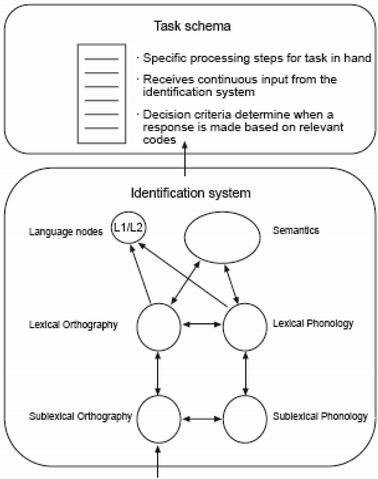
\includegraphics[scale=0.5]{Intro/Figures/biaplus.png}
\caption{The BIA+ model of word recognition \parencite[reprinted from][]{Dijkstra2002}}
\end{center}
\end{figure}

The word identification system deals with linguistic input to the model. The BIA+ posits an integrated lexicon (i.e., the words of each language are integrated into one “dictionary”) and shared semantics across the two languages. The word identification system is highly interactive. Upon “reading” a word, nodes for phonological and orthographic representations at the lexical and sublexical levels become active. Activation then spreads within and between the lexical and sublexical levels causing potential candidates to become more highly activated than other words. The higher levels of the model (i.e., the semantics level and language nodes) receive activation from the lower levels. In the semantic level, concepts receiving enough activation spread this activation back down to the lower levels further reinforcing the activation of potential lexical candidates. The language nodes are responsible for identification of the language being read. A crucial assumption made by the model is that the higher level nodes may only receive bottom-up activation. Furthermore, the language nodes may not send activation back down to the lower levels. Thus, prior knowledge of the intended language will not increase activation to nodes at lower levels. That is, the language nodes cannot function as a language filter. Instead, the nodes must be sufficiently activated through experience with a linguistic input.

While the word identification system handles linguistic input, the task schema deals with non-linguistic contexts. The task schema is responsible for accomplishing the task at hand (e.g., lexical decision, naming, etc.) and determining when a response should be made. In order to help with this decision, this level of the model receives constant input from the word identification system. A critical assumption of the BIA+ model is that the task schema (and, thus, non-linguistic context) does not infiltrate the word recognition system.  Evidence for this was shown by \textcite{Dijkstra2000} who demonstrated that the presence of stimuli and not expectations derived from instructions affected bilingual performance in an LDT.

% Dijkstra, de Bruijn, Schriefers, and ten Brinke (2000)

Given the assumptions of the BIA+ model it is easy to see how cross-language overlap will affect the recognition of words. Cognates, because of their close overlap in orthography, phonology, and meaning, will receive activation in both languages more quickly compared to words without similar overlap. Thus lexical decision or naming will be facilitated. On the other hand, when homographs are the input, the cross-language overlap with orthography and phonology may initially speed activation but the discrepancy in meaning will cause the system to have trouble identifying the language of the word thus slowing lexical decision or naming performance. Overall, the BIA+ predicts that a parallel access account with respect to language occurs in a bottom-up fashion. This parallel activity is not easily constrained by non-linguistic contexts. 

The question now is how linguistic contexts influence word recognition. Because the BIA+ model was designed to account for word recognition outside of sentence contexts, it makes no explicit predictions regarding linguistic contexts. However, as we shall see in the following section, there are specific linguistic contexts that may allow bilinguals to recognize words in a language-selective manner.

\section{In context word recognition}\label{Intro::InContext}
The previous studies reviewed thus far have been conducted asking participants to recognize single words. However, reading rarely involves the recognition of single words without any relation to one another. Instead, words are part of sentences which themselves are part of paragraphs. Likewise in speech, words are components of sentences in a discourse. Each level contributes a new layer of context. Because language use typically occurs in a rich context, out of context experiments provide an artificial environment for reading. For bilinguals, the ambiguity of language membership for each word may also be heightened. This may allow for parallel activation of both languages that would not otherwise exist in an environment with context. More recent research has sought to explore the role of sentence context on bilingual word recognition, investigating whether both language are still activated in parallel when a sentence is in one language alone. Only a handful of studies have examined this question, and the results have been interpreted in a variety of ways.

The fundamental question addressed by this most recent set of studies is whether evidence for nonselectivity can be seen in sentence context. Thus far, every study examining this question has come to the same conclusion: parallel activation does persist even when there is meaningful, unilingual context. This result is amazingly counterintuitive; an English word surrounded by other words that are unambiguously English activates words in another language.  It would seem that language nonselectivity is a fundamental property of the bilingual word recognition system and is does not arise as the result of experimental contexts. 

While the results of all studies converge on the fact that word recognition in sentence context is nonselective, there is disagreement on the issue of whether certain types of linguistic contexts can provide bilinguals a cue to the language of the sentence and work to lessen or even eliminate parallel activation of the unintended language. A set of studies has shown that semantic constraints can, at least sometimes, allow the system to function in a selective manner. The present study attempts to address this debate by examining another type of context that could work similarly to semantic constraints. 

%% The previous work reviewed thus far has been conducted asking participants to recognize single words.  However, reading rarely involves the recognition of single words without any relation to one another. Instead, words are part of sentences which themselves are part of paragraphs with each level contributing a new layer of context. Likewise in speech, words are components of sentences in a discourse. Language use typically occurs in a rich context. Out of context experiments may thus provide an artificial environment devoid of context, where the ambiguity of language membership of each word is heightened allowing parallel activation of both languages. More recent work has sought to explore the role of sentence context on bilingual word recognition, investigating whether both language are still activated in parallel when a sentence is in one language alone. Only a handful of studies have explored this question, and the results have been interpreted in a variety of ways. 

%Some researchers (e.g., Heridia at Psychonomics, and likely Duyck as well) would caution that the results of these in context studies are unclear, painting the picture for each study demonstrating nonselective access in context (e.g., Ducyk 2007, arguably Libben and Titone, Van Assche 2010, Van Assche 2009) there is a study that shows selective access (Schwartz and Kroll, Van Hell, arguably Libben and Titone, Chambers and Cook). However, if we are only allowed to decide that word recognition in sentence context is ``selective'' or ``nonselective'', then the results will appear mixed. If we instead allow language selection to occur on a continuum that ranges from nonselective to selective, then the results become clearer. Under this light, evidence from a variety of converging methodologies confirms that the bilingual word recognition system is, for the most part, nonselective in nature, though there are certain contexts (e.g., highly biased semantic constraints; Schwartz and Kroll, Chambers and Cooke, Libben and Titone) that allow the system to become selective. The selectivity seems to take place during later stages of processing (e.g., semantic integration). Importantly, forcing the system to become selective is not easy (e.g., Van Assche 2010). What has not yet been explored is whether there are other contexts that may allow the word recognition system to select a single language, and whether there exists a context that allows for selective access from the earliest stages in processing.  

\subsection{Evidence for nonselectivity in sentence context}\label{Intro::InContext::Evidence}
There is strong evidence that bilingual word recognition in sentence context is nonselective in nature. This is seen across a variety of methodologies, for example in word naming \parencite[e.g.,][]{Schwartz2006}; in lexical decision and translation \parencite[e.g.,][]{Baten2010, VanHell2008}; in eye-tracking measures of reading \parencite[e.g.,][]{Duyck2007, Libben2009, VanAssche2009, VanAssche2010}; and during auditory word recognition \parencite[][]{Chambers2009}. The unintended language is activated regardless of whether the less dominant L2 is in use \parencite[e.g.,][]{Baten2010,Chambers2009,Duyck2007, Libben2009, Schwartz2006,  VanAssche2010} or the more dominant L1 is use \parencite[e.g.,][]{VanAssche2009, Schwartz2006}. The degree of parallel activation is shown to be a function of the amount of cross-language overlap, suggesting parallel activation is not unique to cognates. Language nonselectivity seems to be a fundamental property of bilingual word recognition system. This finding is quite counterintuitive. It means that despite being aware that a sentence is entirely written in one language, a bilingual will activate both languages. The fact that a sentence has coherent semantics and syntax cannot eliminate activation of the unintended language. However, there is evidence that if a sentence is very strongly biased towards a single interpretation, parallel activity can be modulated.  

%%%% Methodology
Researchers have used a variety of methodologies to study language nonselectivity. Each method can provide a unique perspective on the phenomenon, particularly in what contexts and over what time-course it occurs. Importantly, research shows that regardless of the method used, bilingual word recognition is nonselective in nature. This cross-method comparison is important because it provides support that parallel activation is not task dependent. 

Initial evidence for parallel activation of two languages in sentence context came from behavioral tasks such as word-naming, lexical decision and translation \parencite[e.g.,][]{Baten2010,Schwartz2006, VanHell2008}. Parallel activation has also been demonstrated in auditory word recognition, suggesting that the phenomenon is not specific to written word recognition \parencite[][]{Chambers2009}. While the results of these tasks show the existence of parallel activation, they cannot speak to how early in processing the lexical candidates become activated. Are words in the two languages activated from the very beginning of processing, or do they only become activated during a later stage? The answer to this question comes from evidence from eye-tracking studies. They confirm that both languages are activated in parallel from the earliest stages of processing \parencite[e.g.,][]{Duyck2007, Libben2009, VanAssche2009,  VanAssche2010}. 

\textcite{Schwartz2006} were among the first to investigate bilingual word recognition in sentence context. They asked bilinguals to read sentences in both languages  across separate blocks. The sentences were presented word-by-word at a rapid pace, a method known as rapid serial visual presentation (RSVP). Target cognates and control words were marked in red and remained on the display until the participant spoke the name of the word. The time to begin speaking the word was recorded by a voice trigger. Schwartz and Kroll found that cognates were named faster than their matched controls in both the L1 and the L2. Cognate facilitation suggests that a sentence context is not enough to modulate language nonselectivity; bilinguals activated the lexical representations in both languages while reading in their native and second languages.

These results have also been corroborated by using a different set of behavioral tasks. \textcite{VanHell2008} asked bilinguals to make lexical decisions or to name the translations of target words (cognates or controls) that were embedded in sentences. Again, reaction times to translate or to perform a lexical decision were faster for cognates than for controls, suggesting that bilinguals activated both languages despite target words being embedded in a single language context. Evidence for cross-language activation during  lexical decision was corroborated by \textcite{Baten2010}. While parallel activation in a translation task may not be so surprising (the task demands that both languages are in use and likely to be activated by the participants) a lexical decision task does have this requirement.  Participants in an LDT are likely unaware that knowledge of a second language is important for the experiment. These replications suggest that the parallel activation as witnessed by \textcite{Schwartz2006} cannot be attributed to properties of the task or the materials. Instead, nonselectivity  seems to be a feature of the bilingual word recognition system. 

The finding of nonselectivity is not limited to the written word. \textcite{Chambers2009} show evidence for parallel activation during auditory word recognition. During auditory presentation of  sentences, French-English bilinguals viewed scenes containing 4 objects as their eyes were monitored, a methodology called the Visual World Paradigm (VWP). The visual displays included the target object mentioned in the sentence along with other objects that were unrelated to the sentence. Critical displays contained one object that was a homophone to the target object. For example, a participants might hear ``Marie va d\'{e}crire la \textbf{poule} / [Marie will describe the \textbf{chicken}]'' while viewing a scene that contained a chicken and a pool (the homophone). Chambers and Cooke found that participants were more likely to fixate on distractor homophones (e.g., pool) compared to unrelated objects, suggesting that they were activating English while listening to French sentences auditorily. 

Something that the behavioral studies and the VWP do not tell us is what the nature of the time-course of activation is. How early do participants begin considering options in both languages? If the word recognition system is truly nonselective, then parallel activation should occur immediately.  The use of eye-tracking while participants read sentences is well suited to address this question. 

Eye-tracking allows participants to read sentences naturalistically, as one might read a sentence in a newspaper. Participants are free to read at their own pace, and are able to regress back to earlier parts of the sentence in case something is misunderstood. While reading, the eye-movement patterns of the participants are monitored. The eye-movement record allows for a detailed analysis of the time-course of lexical activation. Early reading measures, such as first fixation duration, provide information about initial lexical access, while later reading measures provide information about semantic integration. 
\textcite{Duyck2007}, \textcite{Libben2009}, \textcite{VanAssche2009}, and \textcite{VanAssche2010} exploit this sensitivity of eye-tracking to show that words are activated in both languages in parallel from the earliest stages of recognition, and that coactivation remains indefinitely. In each of these studies, bilinguals read sentences that contained language-ambiguous words (cognates or homographs) and nonambiguous controls. The studies found that cognate words were fixated on for a shorter amount of time compared to control words while homographs were fixated on for a longer amount of time. Crucially, these effect were present from the earliest measures of reading (e.g., first fixation duration, which is taken to reflect initial lexical access) through later measures that reflect semantic integration. These eye-tracking studies show that during all points of word recognition, bilinguals have both languages activated in parallel.

The results of eye-tracking experiments investigating written and auditory word recognition converge with data from  behavioral studies to show that the finding of parallel activation is not dependent on the methodology being used. Next, we will see that, for the most part, the languages pairs that are used in these experiments and whether the languages are spoken as the L1 or L2 do not affect the overall result of nonselectivity in sentence context. 

%%%% L1-L2 and language pairs
An important consideration in assessing nonselectivity in sentence context is the direction of the coactivation. It is generally assumed that the L1 influences the L2 because the L2 is often the weaker language. However, evidence that the weaker  L2 can influence the stronger L1 provides a compelling case for the ubiquity of nonselectivity. A second consideration is whether the results can be replicated across a variety of language pairs, ensuring that nonselectivity is a feature of bilingual word recognition in general, not just recognition by a specific type of bilingual. Again, the number of in context studies is small, so more replication is necessary, but the preliminary set  suggests that the finding of nonselectivity is invariant to the languages spoken by the bilingual. 

The majority of evidence for nonselectivity in sentence context has been found for bilinguals reading in their L2. \textcite{Baten2010}, \textcite{Duyck2007}, \textcite{VanAssche2010},  \textcite{Libben2009}, and  \textcite{Schwartz2006} all tested bilinguals in English as their L2. \textcite{Chambers2009} recruited bilinguals that use French as their L2. All researchers find evidence for nonselectivity in sentence context. Because, it is often assumed that the L1 has an effect on the L2, parallel activation of the L1 while reading in the L2 may not be surprising. 

Yet, research has shown that bilinguals experience coactivation of the L2 even while reading in the stronger L1, though the number of studies is much more limited. In addition to presenting sentences in the L2, \textcite{Schwartz2006} also asked their participants to read sentences in a block of their L1 (Spanish). Likewise, \textcite{VanAssche2009} eye-tracked participants reading in their native language, Dutch. Both of these studies find cognate effects---evidence for language nonselectivity. These results provide striking evidence that even in L1 reading, a more practiced skill compared to L2 reading, bilinguals activate both languages in parallel. 

Considerably less research has systematically investigated the role of the specific languages in the degree of parallel activation within context. The languages pairs tested thus far have been Dutch and English \parencite[][]{Baten2010,Duyck2007, VanAssche2009, VanAssche2010}, Spanish and English \parencite[][]{Schwartz2006}, and French and English \parencite[][]{Chambers2009,Libben2009}. In the studies that have examined processing in the L2, the L2 has most often been English \parencite[][]{Baten2010,Duyck2007, Libben2009, VanAssche2010}, though Chambers and Cooke studied French as the L2. Because English and French are from different language families (Germanic and Romance) and because results of out of context studies have been replicated across a variety of different language pairs, concerns about confounds due to the language pairs should be ameliorated. Only, two studies have examined processing in the L1, one study investigates processing in Dutch \parencite[][]{VanAssche2009} and another in English \parencite{Schwartz2006}. Both Dutch and English are Germanic languages, which technically could confound the result because of language similarity. However, again results from out of context tasks suggest that the specific languages should not play a very large role; parallel activation should occur regardless of the languages.

A critique of the research supporting nonselectivity is that a majority of the evidence comes from cognates, which arguably have a special representation in the lexicon. Thus the argument can be made that evidence for parallel activation of two languages is really evidence for a special representation of cognates. If this is true, then it sheds doubt on the usefulness of the cognate effect as a measure of cross-language parallel activation. The cognate effect may result from a special representation. This potential confound can be addressed by investigating the role of cross-language overlap in word recognition. If the cognate effect is driven by special representation, then word recognition times should not differ as a function of the degree of overlap because all cognates are special. In contrast, if the cognate effect is really a marker of parallel activation, then we should see graded effects that are dependent on the amount of cross-language overlap.  

A subset of the studies discussed above show evidence that the size of the cognate effect  depends on the degree of cross-language overlap. Cross-language overlap can be operationalized in terms of orthographic overlap and phonological overlap. For example, \textit{hotel} and \textit{ship} are both cognates with Dutch. \textit{Hotel}, however, has complete orthographic overlap with Dutch whereas \textit{ship} is written as \textit{schip} in Dutch, containing a slight difference in orthography. Similarly, words that are written the same across languages often differ in their pronunciation (phonological overlap) or in their meaning (i.e., homographs). The typical finding has been that words with less cross-language overlap tend to elicit slower reaction times while words with greater overlap are recognized faster. This justifies the use cognate effect as a marker of parallel activation. 

\textcite{Duyck2007} conducted a discrete analysis using their eye-tracking data  to show that cross-language overlap affects the presence of the cognate effect. In their materials, they included cognates and noncognate words, and the cognate items were further split into identical cognates (e.g., hotel) and nonidentical cognates (e.g., \textit{ship}-\textit{schip}). Duyck et al. found that identical cognates were fixated on for a shorter amount of time compared to matched noncognate control words. However, this difference was not significant for nonidentical cognates. This finding provides preliminary evidence for the idea that not all cognates are processed equally. Cognates with complete orthographic overlap elicit a greater cognate effect, while the nonidentical cognates elicit a smaller effect. This small effect was apparently not detectable by Duyck et al.'s analysis.  

%An alternative explanation for this lack of cognate effect for nonidentical cognates exists. The sentences in this experiment may have been providing lexical restrictions, albeit weak ones, to language of the sentence. The effect of these restrictions in negating parallel activity only emerged when parallel activation was weaker because of incomplete orthographic overlap. This alternate explanation is complementary to the hypothesis that incomplete orthographic overlap alone is the determinant of the lack of cognate effect. However, it is important to disentangle the role, if any, that the sentence context plays from the role that orthographic overlap plays in parallel activation of two languages. 

%Duyck et al. (2007) conducted two control studies (out of context lexical decision and in context lexical decision) to provide support the idea that the lack of a cognate effect for nonidentical cognates is due to orthographic overlap  and not to sentential context. They showed that LDT reaction times to cognate words (in and out of context) were influenced by the degree of orthographic overlap: a decrease in orthographic overlap resulted in greater reaction times. This correlation also held for reading times in the eye-tracking experiment. Yet, in both LDTs there was still a significant cognate effect for the nonidentical cognates where there was none in the eye-tracking experiment. The presence of a cognate effect for nonidentical cognates sentential LDT suggests that the nonidentical cognates, though they lacked complete orthographic overlap, were sufficiently able to elicit parallel activation of both languages in the context of a sentence. 

%The presence of parallel activation for nonidentical cognates in the sentential lexical decision task leaves open the possibility that the eye-movement record was unable to detect weak parallel activation despite the common assumption that eye-tracking is a more sensitive measure than behavioral tasks. This could occur, counterintuitively, because the method is very sensitive, providing very fast reaction times (on the order of 200ms in Duyck et al., 2007) in comparison to LDT reaction times (around 700ms) for example. Such small effects may be difficult to detect with very fast reaction times and instead may require a measure that magnifies the differences, something to be kept in mind when designing a study that might result in small effects. Overall, the results of the series of studies conducted by Duyck et al. suggest that a sentence context alone is not sufficient to override parallel activation of the L1 when reading in the L2.

%The authors show that the degree of parallel activation is a function of cross-language overlap. Cognates that have greater orthographic overlap across languages tend to be read faster. Duyck et al. conduct a  discrete analysis by comparing nonidentical cognates to identical cognates and show that only identical cognates provide evidence for parallel activation. This finding is honed by Van Assche et al. who conduct a regression analysis to show that this effect is actually continuous: the cognate effect decreases continually as a function of orthographic overlap.

While the results of \textcite{Duyck2007} suggest that orthographic overlap influences the time to identify a word, a discrete difference between identical and nonidentical cognates does not defeat the theory that cognates have a special representation. One could argue that while identical cognates are specially represented, nonidentical cognates are not cognates are not, explaining why \textcite{Duyck2007}  not see facilitation for nonidentical cognates. A more fine grained analysis can adjudicate whether cognates are somehow special.

\textcite{VanAssche2009} and \textcite{VanAssche2010} found continuous effects of cross-lingual overlap on reading times in the L1 and in the L2. Where \textcite{Duyck2007} categorized cognates into discrete groups (identical and nonidentical), \textcite{VanAssche2009} calculated the orthographic overlap of each target word and its translation according to the method by \textcite{VanOrden1987}. This method provides a numerical measure of overlap between two words by taking into account such factors as number of letters, number of paired adjacent letters, whether the words share the same first or last letter, etc. This measure of overlap was then entered as a predictor into linear mixed-effects regression models for each of the eye-tracking measures of interest (first fixation duration, gaze-duration, and regression-path duration). While overall model fits were not included in the results, the authors found a significant effect of orthographic overlap on reading times. The time to read a word was inversely proportional to the degree of overlap; as overlap decreased reading times increased. This shows that readers utilized this  lexical information during word recognition. 

\textcite{VanAssche2010} further show that the degree of phonological overlap influences bilingual word recognition and can be used as another continuous  measure of cognate status. They measured the degree of phonological overlap  by asking a group of participants, independent from their main experiments, to rate how similarly a word and its translation sounded. These ratings were aggregated to determine degree of overlap. When phonological similarity was entered into the regression model, the authors found an inversely proportional relation to reaction times, similar to that of orthographic overlap.

The results of \textcite{Duyck2007}, \textcite{VanAssche2009}, and \textcite{VanAssche2010} illustrate that the degree of cross-lingual overlap  influences how bilinguals recognize words in sentence context and that this effect is continuous. As words across two language increase in the degree of overlap, the speed at which they are recognized increases. This finding is important because it shows that cognate status per se is not what influences recognition. Recognition is influenced by the degree of overlap between a word and its translation equivalent. Therefore it is correct to assume that the cognate effect is a measure of parallel activation of the bilingual's two languages not as proof of a special representation of cognates.

Taken together, the results of the in context studies presented here all show that language nonselectivity cannot be overcome by a sentence context alone. Words become activated in both languages according to their degree of overlap across languages despite the coherence created by the semantics, syntax, and language of a sentence. The parallel activation is so pervasive that it persists while bilinguals read sentences in their stronger native language, not only during L2 reading.  

Yet it would seem that at some point, a bilingual should be able to ``choose'' a language. After all, bilinguals can successfully make lexical decisions in a sentence context, nor do they have a problem assembling the meaning of a sentence. Given the pervasiveness of nonselectivity in sentence context, a second goal of in context word recognition research has been to explore whether there are any linguistic factors that might allow bilinguals to make a language selection.

\subsection{The role of semantic constraints}\label{Intro::InContext::SemanticConstraints}
While all studies converge on the finding that word recognition is nonselective within a sentence context, they diverge on whether recognition may become selective under certain conditions, namely following a highly constrained semantic context. A subset of the studies examined above illustrates that patterns of word recognition following a highly biased context are consistent with the predictions made by a language-selective access account. In highly constrained  contexts, cognate facilitation is eliminated \parencite[the \textit{semantic constraint effect}; e.g.,][]{Chambers2009,Libben2009, Schwartz2006, VanHell2008}. However, there is disagreement in the literature as to whether the locus of the effect actually stems from language-selectivity, or whether it is the result of another factor, such as a confounding of the methods or a floor effect caused by the speeded processing due to semantic constraints. Furthermore, one study has failed to find the semantic constraint effect \parencite[e.g.,][]{VanAssche2010}. Despite the criticisms of semantic constraints, the effect seems to be reliable. Yet, semantic constraints cannot be the only way that a bilingual comes to choose a language. After all, not every sentence is highly semantically constrained. Other factors that provide language-specific cues, such as the syntax, may induce language-selective access.   

The semantic constraint effect has been replicated with a variety of methods including lexical decision and translation \parencite[][]{VanHell2008}, eye-tracking during reading, and with the Visual World Paradigm \parencite[][]{Chambers2009,Libben2009}. The eye-tracking record shows that when semantic constraints have an effect, it occurs during later stages in processing \parencite[][]{Libben2009}. Because the effect of semantic constraints can be seen with a variety of methods, from behavioral to eye-tracking, the effect is likely not due to the methodology. However, the debate about whether speeded processing creates a floor effect is still open. The current study will approach the question of whether word recognition can become selective by investigating whether another sentential factor, language-specific syntactic constraints, can eliminate or reduce parallel activation. 

\textcite{Schwartz2006} demonstrate that a sentence which is highly constrained in its interpretation appears to eliminate the cognate effect. Schwartz and Kroll varied the semantic constraint of their sentences such that half of the sentences contained a highly predictable semantic contexts (i.e., \textit{high constraint}) while the other half did not (i.e., \textit{low constraint}). Constraintedness was determined by an offline sentence completion task. The target word of each sentence was removed along with any material following the target. A set of participants who did not complete the main experiment  asked to complete each sentence. If the participants were highly likely to complete a sentence with the actual target word, the sentence was rated as high constraint. If a variety of words followed a sentence, it was rated as low constraint. 

\textcite{Schwartz2006} found cognate facilitation only in the low constraint sentences. In sentences with a high semantic constraint, the authors found that all target words were named faster. This signifies that the biased context helped participants to access the upcoming target word. Importantly, the authors failed to find a cognate effect for target words following a high semantic constraint.  The cognate facilitation effect in low constraint sentences signifies that a sentence context alone is not enough to constrain word recognition to one language. However, additional semantic cues may provide lexical restrictions to language, resulting in a modulation the cognate effect. 

The finding of apparent selective access in high constraint sentences has been criticized on two grounds. First,  the elimination of the cognate effect may be the result of the method that Schwartz and Kroll used to investigate word recognition (i.e., word naming). Second, the elimination of the cognate effect in high constraint sentences may be the result of the facilitation that occurs following a biased semantic context. That is, because high constraint sentences speed lexical access, word recognition in these sentences may reach a floor and  cognate facilitation may no longer be witnessed. Each critique warrants further explorations, and with the use of converging methodologies, they can begin to be addressed. 

%%%% Methods
The semantic constraint effect cannot be due to the methods used by \textcite{Schwartz2006}. The effect has been replicated using other behavioral methods as well as with eye-tracking methods \parencite[e.g.,][]{Chambers2009,Libben2009,VanHell2008}. The eye-tracking record during reading suggests that the effect of semantic constraints occurs during later stages of word recognition, meaning that word recognition is initially nonselective. While converging methods confirm that semantic constraints eliminate the cognate effect, they cannot confirm that this modulation is due to language-selective access. The reduction in the cognate effect may be due to speeded access of semantic constraints creating a floor effect that over-shadows an effect of cross-language overlap. 

\textcite{VanHell2008} show that semantic constraints modulate the cognate effect during word recognition while bilinguals read sentences and were asked to make either a lexical decision or to translate the target words. When targets followed a high semantic constraint (which again facilitated reaction times to identify targets), the difference between cognates and controls was reduced, and in lexical decision the difference was eliminated. A similar finding occurred during auditory word recognition. \textcite{Chambers2009} found  that following sentences containing a high semantic constraint, fixations toward homograph distractor pictures were greatly decreased when compared to fixations in low constraint sentences. 

Following highly semantically constrained sentences, the degree to which both languages were activated was greatly decreased in line with the findings of Schwartz and Kroll. Because the constraint effect was replicated with a different set of behavioral methods, it signifies that the findings of Schwartz and Kroll did not depend on the word naming method they used. 

%Like Schwartz and Kroll (2006), Van hell and de Groot included sentences that had a high semantic constraint in their materials. Recall that they asked one group of participants to make  a lexical decision on the target words while translated the targets and that translation and lexical decisions were faster for cognates when the sentences were low semantic constraint. Crucially, w

Behavioral tasks, such as lexical decision, translation, and word naming, rely on the response made by a participant to a stimulus. Responses  tell us about the later stages of word recognition---the end result of the process. Information about the  earliest stages of the process is potentially lost. Thus, it is conceivable that in high constraint sentences, word recognition  proceeds in an initially nonselective manner and then becomes selective downstream. If this theory were true, behavioral methods such as those used by \textcite{Schwartz2006} and \textcite{VanHell2008} might fail to capture evidence for this initial nonselectivity. While the Visual World Paradigm used by \textcite{Chambers2009} provides a good temporal measure of the word candidates participants are considering, the analysis they conducted was not fine-grained enough discern whether the semantic constraint effect began initially or later on. Analyses of fixations during sentence reading are sensitive enough to adjudicate between early and late processing differences.  
 
\textcite{Libben2009} provide striking data that suggest word recognition in high constraint sentences proceeds in an initially nonselective manner but becomes selective over time as the meaning of the sentence is integrated. They show that in high constraint sentences cross-language facilitation and inhibition were only present in early measures of reading (e.g., first-fixation duration). Later measures (e.g., regression path) showed no significant differences between language-ambiguous stimuli and control words. This result highlights the fact that the word recognition system is profoundly nonselective at early stages of processing, but that semantic constraints can allow the system to become selective over time. It also further shows that the semantic constraint effect is not unique to behavioral methods, such as word naming. 

Findings from a variety of methods provide evidence that semantic constraints can eliminate activation from the unintended language. This finding is not method-specific, though there are differences in how methods illustrate details about the time-course of processing. While the semantic constraint effect is not due to the methodology used,  locus of the effect is still in question; the elimination of the cognate effect may be due to the fact that semantic biases increase word recognition speed. This speed increase may create a floor effect that diminishes the detectability of the cross-language activity. 

%%%% Speed of semantic constraints
Semantic constraints reliably increase the rate at which upcoming words are recognized, and we have seen that semantic constraints decrease or eliminate effects that are known to measure parallel activation (e.g., cognate effect and homograph inhibition). However, the locus of this modulation is in question. It could stem from two possible sources: language-selective access cause by increased lexical cues due to the constraint, or, more trivially, a loss of analytical power due to the decrease in reaction times due to the semantic constraint. Much of the prior research cannot address this question, except for, possibly, the results of Van Hell and De Groot.  

The idea behind the floor effect theory is that participants become so fast at predicting an upcoming word, the cognate effect can no longer be measured. Cross-language activation is still present, however the effect size is so small it cannot be measured. This theory can be tested by examining a situation in which there is a semantic constraint but no floor effect. In such a situation, the theory would predict that a cognate effect would be present, and the magnitude of the effect should be no different than in a low constraint sentence. A difference in the sizes of the cognate  effects would indicate that the semantic constraint is in some way affecting the degree of parallel activation.

The translation task of \textcite{VanHell2008} provides the situation outlined above. In their experiments, participants translated target words that were embedded in high and low constraint sentences. Translation is a more difficult task for participants compared to lexical decision or word naming. Hence, reaction times are slower (though no statistical analyses were conducted to test this). Because reaction times were no longer at floor, role of semantic constraints can be investigated. Van Hell and De Groot found cognate effects in both high and low constraint sentences during translation. However, counter to the predictions made by the floor effect theory, the cognate effect was smaller in the high constraint condition, indicating that although participants coactivated both languages during the translation, this coactivation was less when the context was biased towards a single interpretation. This modulation is likely due to a decrease in parallel activation and not a floor effect because reaction times in the task were slower overall. 

%%%% Failure to find semantic constraints
Not all studies have managed to find evidence for the semantic constraint modulation of the cognate effect. Though, failure to find an effect is not evidence that no effect exists, especially in the presence of other positive evidence. It may be that semantic constraints do not always allow for words to be selectively accessed from the lexicon. 

\textcite{VanAssche2010} failed to find evidence that semantic constraints modulate the cognate effect, despite the inclusion of  sentences that were rated as being very high constraint compared to previous studies. Instead, their Dutch-English bilinguals read cognate words significantly faster than noncognate words in both low and high constraint sentences; the magnitude did not change. According to Van Assche et al. ``this contrasts with Libben and Titone (2009) who found cognate facilitation only in early comprehension measures... Instead, our results suggest that the influence of such factors on the language-selectivity of lexical access is rather limited...'' This result also contrasts with Schwartz and Kroll, Van Hell and De Groot, and Chambers and Cooke. As we know from statistics, lack of a significant effect is not evidence that there is no effect. Instead there are likely many factors which the authors did not consider that likely result in the lack of the effect.  

The main reason that \textcite{VanAssche2010} failed to find an effect was likely due to the sizes of their cognate effects. For some of the measures, the effects were less than 10ms. These effects are so small that the number of participants they recruited is much higher than in previous studies (e.g., 60 participants). A sub-10 ms effect, in  addition to potentially not being a meaningful difference, leaves less room to find a detectable interaction when the effect is expected to decrease.

In this study, the more proficient language and dominant language (i.e., Dutch) of the environment was inactive, so cognate effects should have been rather large \parencite[e.g.,][]{Jared2001, Marian2003, VanHell2002}. Why were the effects so small?  \textcite{VanAssche2010} chose to use exclusively nonidentical cognates as a tool to measure of parallel activation. As we saw earlier, nonidentical cognates tend to elicit less parallel activation (and perhaps none at all) because of their lack in cross-language overlap. Furthermore, in \textcite{Duyck2007} the group failed to find any cognate effects on nonidentical cognates as a group. In this light, it is not surprising that Van Assche et al. struggled to find a cognate effect and failed to finsd evidence for an interaction. 

While failure to find the semantic constraint modulation does not prove that the effect does not exist, the findings of \textcite{VanAssche2010} do suggest that decreasing parallel activation is not always as easy as including a high semantic constraint. Furthermore, not every sentence contains a semantic constraint, thus there may be several other factors that allow bilinguals to come to a language decision. 

\section{The present investigation}\label{Intro::PresentInvestigation}
Most researchers assume that the semantics is shared across language. Therefore there is no reason a priori that the meaning of a sentence should provide strong language cues. On the other hand, it is well known that syntax differs across languages. If any linguistic construct should provide language cues, then it should be the syntax. The goal of the  present investigation  is to  explore whether language-specific syntactic constraints allow for language-selective access. While nobody has examined this question, there is evidence from an out of context task and an in context task that hints that aspects of the syntax may be important during word recognition.

\textcite{Sunderman2006} showed that grammatical class differences (a morphosyntactic property) can reduce lexical form interference from the other language. Relatively proficient English-Spanish speakers made translation recognition judgments about word pairs in Spanish and English (i.e., ``Are these two words translations of one another?''). Critical word pairs required a ``no'' response, and a subset of critical items were related in lexical form (e.g., \textit{mano}-\textit{man}). When the two words belonged to the same grammatical class (e.g., noun-noun),  Sunderman and Kroll found lexical interference compared to control items (e.g., \textit{casa}-\textit{man}). However, when the two words differed in their grammatical classes (e.g., noun-verb), the lexical interference was dramatically reduced, suggesting that the degree of lexical interference depended on grammatical class overlap. 

A similar result was found by \textcite{Baten2010} for bilingual participants reading in sentence context. Participants performed an English lexical decision for target words embedded in sentences. Homographs elicited a facilitation effect when the homograph and its translation shared grammatical class, suggesting that both languages were activated. However, when the grammatical class differed across the two languages the facilitation effect was eliminated, consistent with language-selective access. The results of \textcite{Sunderman2006} and \textcite{Baten2010}  hint that syntax may play a role in modulating  influence from the unintended language.

The present investigation explores the role of syntax in allowing for language-selective activation by asking Spanish-English bilinguals to read sentences that are language-specific to Spanish in their syntax. We operationalize Spanish-specific syntactic constraints as the inclusion of proclitics and the dropping of the subject of an object relative clause before the target word of the sentence is reached. Spanish-specific syntax is exemplified in \ref{lasmonjas2} (target word: \textit{directora}, a cognate).

\ex.\label{lasmonjas2} Las monjas \textbf{le} llevaron las mantas que \textbf{[pro]} hab\'{i}an bordado a la directora del orfanato.\\
      The nuns \textbf{[ ]} took the quilts that \textbf{they} had embroidered to the director of the orphanage.

If the presence of Spanish-specific syntactic constructions in a sentence allow the reader or listener \textit{zoom in} to the target
language \parencite[e.g.,][]{Elston-Guttler2005}, then word recognition should proceed in a language-selective selective manner. That is, cognates
embedded in sentences with language-specific syntax (and with a low
semantic bias) should be accessed as if they are a word only in the
language of that sentence (i.e., a noncognate word). However, following language-general syntax, word recognition should proceed in a nonselective manner, in line with previous studies. Monolingual control experiments will confirm that any cognate or syntactic specificity effects are due to the experimental manipulations and not to idiosyncratic properties of the stimuli.

The experiments in the current investigation are laid out as follows. Experiment 1 implements a word naming task to replicate the cognate facilitation effect outside of sentence context. Experiment 2 uses the Rapid Serial Visual Presentation task to present cognate and noncognate control words in sentence contexts that contain language-general (low syntactic constraint) and language-specific syntactic constraints (high syntactic constraint). A block of Spanish sentences will contain both low and high syntactic constraints while a block of English sentences contain only low syntactic constraints. Experiments 3 and 4 are English and Spanish monolingual control experiments.  


\chapter{General directions and methodologies}\label{Roadmap}
There were two main goals to this study. The first goal was to further confirm that a sentence context is not enough by itself to constrain word recognition to one language. The second goal of the study was to assess whether the use of language-specific syntactic constraints in sentence contexts is sufficient to allow for language-selective word recognition. To investigate these issues, participants performed a Rapid Serial Visual Presentation (RSVP) experiment (Chapter \ref{SEInContext}) in which they read sentences presented word-by-word and named target words aloud. The target words were embedded in sentence contexts that contained syntax specific to Spanish or contained language-general syntax.  Control studies ensured that any effects are due to the intended manipulations and not to idiosyncratic properties of the stimuli. A variety of cognitive tasks and language-proficiency tasks were implemented to insure that our groups of participants were matched for language experience and cognitive performance. These  measures were also  used to explore the ways in which individual differences influence processing. The current chapter provides an overview of the participants recruited and the experimental procedures used in each part of study.

\section{Participants}\label{Roadmap::Participants}
Four groups of participants were recruited for this investigation. Bilinguals who were native speakers of English and acquired Spanish as a second language (English-Spanish bilinguals) were recruited for the out-of context naming study in Chapter \ref{ESOOC}. Native speakers of Spanish who learned English as a second language (Spanish-English bilinguals) participated in the RSVP experiment in Chapter \ref{SEInContext}. Two monolingual control groups were  recruited for the in context control experiment: a group of English monolinguals and a group of Spanish monolinguals. The Spanish monolinguals were recruited from the University of Granada in Spain, while all other groups were recruited from the Pennsylvania State University in the United States. 

The learners of Spanish studying at Penn State University were recruited for the out of context task in Chapter \ref{ESOOC} in order to ensure that our cognates were sensitive to parallel activation of two languages. Because the size of the cognate effect is typically larger for participants using their second language, a failure to find effect in the second language would indicate that effects would not likely be found for participants reading in their native language. 

Native speakers of Spanish were necessary for the main experiment in Chapter \ref{SEInContext} because our critical manipulation depends on speakers' knowledge of and ability to process complex syntactic structures in Spanish. Hence, a  high proficiency in Spanish was required. While high proficiency L2 speakers certainly exist, some researchers argue that L2 speakers do not have access to certain syntactic structures in the L2 \parencite[e.g.,][]{Clahsen2006}. While I remain agnostic towards this claim, the choice of native Spanish speakers ensures that they will be able to process the structures that the critical manipulation depends on. 

In order to ensure that any effects found were due to the intended manipulations, two groups of monolinguals were recruited to participate in each of the language blocks. A group of Spanish monolinguals recruited from the University of Granada, Spain read the Spanish portion of the in context study. A group of English monolinguals from Penn State were recruited to read the English portion of the materials. Because monolinguals only know one language, they should not demonstrate any effects due to cognate status. 

\section{Word naming tasks}
The word naming tasks were used to assess the degree of cross-language activation. Participants were presented with cognate and control words, and the time it took them to begin naming was recorded.  The latencies for cognates and noncognates were compared to measure parallel activation. Two types of word naming tasks were used in the present set of experiments: out of context word naming, and word naming in sentence context. Before detailing each of these tasks, I review how the target words were selected. 

\subsection{Selection of target words}
A set of 64 cognates between English and Spanish were selected. Each of the cognates was matched to a Spanish noncognate control word, yielding a total of 128 target words. The targets were matched for  word frequency \parencite[e.g.,][]{Alameda1995}, length, number of syllables, number of phonemes, first phoneme, and animacy. Cognates and controls were not always perfectly matched for every measure, but importance was placed on frequency and length. Neither length nor frequency differed significantly between Spanish cognate and noncognate words (both \textit{t}(126) $< 1$). These  target words were  then translated into English. The English cognate and control materials are reproduced in tables Table \ref{eng_cognates} and Table \ref{eng_controls}. Again, neither length nor frequency differed significantly between the cognate and control words. The cognate materials and control stimuli are reproduced in Appendix \ref{Appendix::OOC}.

%% \begin{centering}
%% % latex.table(x = as.matrix(cogs), file = "cogs", longtable = T) 
%
\setlongtables
\begin{longtable}{|l|c|c|c|c|c|c|}
\hline
\multicolumn{1}{|c|}{Cognate}&\multicolumn{1}{c|}{Frequency}&\multicolumn{1}{c|}{First.Phoneme}&\multicolumn{1}{c|}{Syllables}&\multicolumn{1}{c|}{Phonemes}&\multicolumn{1}{c|}{Length}&\multicolumn{1}{c|}{Animacy}\\ \hline
\endhead
\hline\endfoot
bus~~~~~~~~~~&~~2~~~~~~~~~~&b~~~~~~~~~~~~&1~~~~~~~~~~~~&~3~~~~~~~~~~~&~3~~~~~~~~~~~&i~~~~~~~~~~~~\\ 
general~~~~~~&632~~~~~~~~~~&x~~~~~~~~~~~~&3~~~~~~~~~~~~&~7~~~~~~~~~~~&~7~~~~~~~~~~~&a~~~~~~~~~~~~\\ 
colegas~~~~~~&~56~~~~~~~~~~&k~~~~~~~~~~~~&3~~~~~~~~~~~~&~7~~~~~~~~~~~&~7~~~~~~~~~~~&a~~~~~~~~~~~~\\ 
garaje~~~~~~~&~22~~~~~~~~~~&g~~~~~~~~~~~~&3~~~~~~~~~~~~&~6~~~~~~~~~~~&~6~~~~~~~~~~~&i~~~~~~~~~~~~\\ 
cable~~~~~~~~&~16~~~~~~~~~~&k~~~~~~~~~~~~&2~~~~~~~~~~~~&~5~~~~~~~~~~~&~5~~~~~~~~~~~&i~~~~~~~~~~~~\\ 
proyecto~~~~~&155~~~~~~~~~~&p~~~~~~~~~~~~&3~~~~~~~~~~~~&~8~~~~~~~~~~~&~8~~~~~~~~~~~&i~~~~~~~~~~~~\\ 
c\'{a}mara~~~~~~~&114~~~~~~~~~~&k~~~~~~~~~~~~&3~~~~~~~~~~~~&~6~~~~~~~~~~~&~6~~~~~~~~~~~&i~~~~~~~~~~~~\\ 
turistas~~~~~&~51~~~~~~~~~~&t~~~~~~~~~~~~&3~~~~~~~~~~~~&~8~~~~~~~~~~~&~8~~~~~~~~~~~&a~~~~~~~~~~~~\\ 
jirafa~~~~~~~&~~2~~~~~~~~~~&x~~~~~~~~~~~~&3~~~~~~~~~~~~&~6~~~~~~~~~~~&~6~~~~~~~~~~~&a~~~~~~~~~~~~\\ 
reportero~~~~&~~3~~~~~~~~~~&r~~~~~~~~~~~~&4~~~~~~~~~~~~&~9~~~~~~~~~~~&~9~~~~~~~~~~~&a~~~~~~~~~~~~\\ 
plato~~~~~~~~&~85~~~~~~~~~~&p~~~~~~~~~~~~&2~~~~~~~~~~~~&~5~~~~~~~~~~~&~5~~~~~~~~~~~&i~~~~~~~~~~~~\\ 
pirata~~~~~~~&~12~~~~~~~~~~&p~~~~~~~~~~~~&3~~~~~~~~~~~~&~6~~~~~~~~~~~&~6~~~~~~~~~~~&a~~~~~~~~~~~~\\ 
pipa~~~~~~~~~&~38~~~~~~~~~~&p~~~~~~~~~~~~&2~~~~~~~~~~~~&~4~~~~~~~~~~~&~4~~~~~~~~~~~&i~~~~~~~~~~~~\\ 
planta~~~~~~~&~89~~~~~~~~~~&p~~~~~~~~~~~~&2~~~~~~~~~~~~&~6~~~~~~~~~~~&~6~~~~~~~~~~~&a~~~~~~~~~~~~\\ 
profesora~~~~&~15~~~~~~~~~~&p~~~~~~~~~~~~&4~~~~~~~~~~~~&~9~~~~~~~~~~~&~9~~~~~~~~~~~&a~~~~~~~~~~~~\\ 
estatua~~~~~~&~36~~~~~~~~~~&E~~~~~~~~~~~~&3~~~~~~~~~~~~&~7~~~~~~~~~~~&~7~~~~~~~~~~~&i~~~~~~~~~~~~\\ 
cliente~~~~~~&~40~~~~~~~~~~&k~~~~~~~~~~~~&2~~~~~~~~~~~~&~7~~~~~~~~~~~&~7~~~~~~~~~~~&a~~~~~~~~~~~~\\ 
cobra~~~~~~~~&~37~~~~~~~~~~&k~~~~~~~~~~~~&2~~~~~~~~~~~~&~5~~~~~~~~~~~&~5~~~~~~~~~~~&a~~~~~~~~~~~~\\ 
cubo~~~~~~~~~&~26~~~~~~~~~~&k~~~~~~~~~~~~&2~~~~~~~~~~~~&~4~~~~~~~~~~~&~4~~~~~~~~~~~&i~~~~~~~~~~~~\\ 
organizador~~&~~4~~~~~~~~~~&O~~~~~~~~~~~~&5~~~~~~~~~~~~&11~~~~~~~~~~~&11~~~~~~~~~~~&a~~~~~~~~~~~~\\ 
viol\'{i}n~~~~~~~&~17~~~~~~~~~~&b~~~~~~~~~~~~&2~~~~~~~~~~~~&~6~~~~~~~~~~~&~6~~~~~~~~~~~&i~~~~~~~~~~~~\\ 
c\'{i}rculo~~~~~~&~59~~~~~~~~~~&T~~~~~~~~~~~~&3~~~~~~~~~~~~&~7~~~~~~~~~~~&~7~~~~~~~~~~~&i~~~~~~~~~~~~\\ 
pistola~~~~~~&~50~~~~~~~~~~&p~~~~~~~~~~~~&3~~~~~~~~~~~~&~7~~~~~~~~~~~&~7~~~~~~~~~~~&i~~~~~~~~~~~~\\ 
oficial~~~~~~&118~~~~~~~~~~&O~~~~~~~~~~~~&3~~~~~~~~~~~~&~7~~~~~~~~~~~&~7~~~~~~~~~~~&a~~~~~~~~~~~~\\ 
problemas~~~~&279~~~~~~~~~~&p~~~~~~~~~~~~&3~~~~~~~~~~~~&~9~~~~~~~~~~~&~9~~~~~~~~~~~&i~~~~~~~~~~~~\\ 
computadora~~&~~9~~~~~~~~~~&k~~~~~~~~~~~~&5~~~~~~~~~~~~&11~~~~~~~~~~~&11~~~~~~~~~~~&i~~~~~~~~~~~~\\ 
detective~~~~&~12~~~~~~~~~~&d~~~~~~~~~~~~&4~~~~~~~~~~~~&~9~~~~~~~~~~~&~9~~~~~~~~~~~&a~~~~~~~~~~~~\\ 
atleta~~~~~~~&~~8~~~~~~~~~~&A~~~~~~~~~~~~&3~~~~~~~~~~~~&~6~~~~~~~~~~~&~6~~~~~~~~~~~&a~~~~~~~~~~~~\\ 
compositor~~~&~~4~~~~~~~~~~&k~~~~~~~~~~~~&4~~~~~~~~~~~~&10~~~~~~~~~~~&10~~~~~~~~~~~&a~~~~~~~~~~~~\\ 
coronel~~~~~~&~~6~~~~~~~~~~&k~~~~~~~~~~~~&3~~~~~~~~~~~~&~7~~~~~~~~~~~&~7~~~~~~~~~~~&a~~~~~~~~~~~~\\ 
paciente~~~~~&~52~~~~~~~~~~&p~~~~~~~~~~~~&3~~~~~~~~~~~~&~8~~~~~~~~~~~&~8~~~~~~~~~~~&a~~~~~~~~~~~~\\ 
hamburguesa~~&~~3~~~~~~~~~~&A~~~~~~~~~~~~&4~~~~~~~~~~~~&~9~~~~~~~~~~~&11~~~~~~~~~~~&i~~~~~~~~~~~~\\ 
capitales~~~~&~13~~~~~~~~~~&k~~~~~~~~~~~~&4~~~~~~~~~~~~&~9~~~~~~~~~~~&~9~~~~~~~~~~~&i~~~~~~~~~~~~\\ 
sopa~~~~~~~~~&~31~~~~~~~~~~&s~~~~~~~~~~~~&2~~~~~~~~~~~~&~4~~~~~~~~~~~&~4~~~~~~~~~~~&i~~~~~~~~~~~~\\ 
vendedor~~~~~&~21~~~~~~~~~~&b~~~~~~~~~~~~&3~~~~~~~~~~~~&~8~~~~~~~~~~~&~8~~~~~~~~~~~&a~~~~~~~~~~~~\\ 
decisi\'{o}n~~~~~&140~~~~~~~~~~&d~~~~~~~~~~~~&4~~~~~~~~~~~~&~8~~~~~~~~~~~&~8~~~~~~~~~~~&i~~~~~~~~~~~~\\ 
rata~~~~~~~~~&~34~~~~~~~~~~&r~~~~~~~~~~~~&2~~~~~~~~~~~~&~4~~~~~~~~~~~&~4~~~~~~~~~~~&a~~~~~~~~~~~~\\ 
su\'{e}ter~~~~~~~&~~6~~~~~~~~~~&s~~~~~~~~~~~~&2~~~~~~~~~~~~&~6~~~~~~~~~~~&~6~~~~~~~~~~~&i~~~~~~~~~~~~\\ 
ingeniero~~~~&~70~~~~~~~~~~&I~~~~~~~~~~~~&4~~~~~~~~~~~~&~9~~~~~~~~~~~&~9~~~~~~~~~~~&a~~~~~~~~~~~~\\ 
beb\'{e}~~~~~~~~~&~30~~~~~~~~~~&b~~~~~~~~~~~~&2~~~~~~~~~~~~&~4~~~~~~~~~~~&~4~~~~~~~~~~~&a~~~~~~~~~~~~\\ 
%\newpage
instituto~~~~&~84~~~~~~~~~~&I~~~~~~~~~~~~&4~~~~~~~~~~~~&~9~~~~~~~~~~~&~9~~~~~~~~~~~&i~~~~~~~~~~~~\\ 
tanque~~~~~~~&~12~~~~~~~~~~&t~~~~~~~~~~~~&2~~~~~~~~~~~~&~5~~~~~~~~~~~&~6~~~~~~~~~~~&i~~~~~~~~~~~~\\ 
director~~~~~&173~~~~~~~~~~&d~~~~~~~~~~~~&3~~~~~~~~~~~~&~8~~~~~~~~~~~&~8~~~~~~~~~~~&a~~~~~~~~~~~~\\ 
estrategia~~~&~54~~~~~~~~~~&E~~~~~~~~~~~~&4~~~~~~~~~~~~&10~~~~~~~~~~~&10~~~~~~~~~~~&i~~~~~~~~~~~~\\ 
caf\'{e}~~~~~~~~~&210~~~~~~~~~~&k~~~~~~~~~~~~&2~~~~~~~~~~~~&~4~~~~~~~~~~~&~4~~~~~~~~~~~&i~~~~~~~~~~~~\\ 
catedral~~~~~&~58~~~~~~~~~~&k~~~~~~~~~~~~&3~~~~~~~~~~~~&~8~~~~~~~~~~~&~8~~~~~~~~~~~&i~~~~~~~~~~~~\\ 
tel\'{e}fono~~~~~&186~~~~~~~~~~&t~~~~~~~~~~~~&4~~~~~~~~~~~~&~8~~~~~~~~~~~&~8~~~~~~~~~~~&i~~~~~~~~~~~~\\ 
carpintero~~~&~12~~~~~~~~~~&k~~~~~~~~~~~~&4~~~~~~~~~~~~&10~~~~~~~~~~~&10~~~~~~~~~~~&a~~~~~~~~~~~~\\ 
brócoli~~~~~~&~~1~~~~~~~~~~&b~~~~~~~~~~~~&0~~~~~~~~~~~~&~0~~~~~~~~~~~&~7~~~~~~~~~~~&a~~~~~~~~~~~~\\ 
caramelos~~~~&~15~~~~~~~~~~&k~~~~~~~~~~~~&4~~~~~~~~~~~~&~9~~~~~~~~~~~&~9~~~~~~~~~~~&i~~~~~~~~~~~~\\ 
familia~~~~~~&495~~~~~~~~~~&f~~~~~~~~~~~~&3~~~~~~~~~~~~&~7~~~~~~~~~~~&~7~~~~~~~~~~~&a~~~~~~~~~~~~\\ 
presidente~~~&138~~~~~~~~~~&p~~~~~~~~~~~~&4~~~~~~~~~~~~&10~~~~~~~~~~~&10~~~~~~~~~~~&a~~~~~~~~~~~~\\ 
estudiante~~~&~37~~~~~~~~~~&E~~~~~~~~~~~~&4~~~~~~~~~~~~&10~~~~~~~~~~~&10~~~~~~~~~~~&a~~~~~~~~~~~~\\ 
recepcionista&~~3~~~~~~~~~~&r~~~~~~~~~~~~&5~~~~~~~~~~~~&11~~~~~~~~~~~&13~~~~~~~~~~~&a~~~~~~~~~~~~\\ 
sof\'{a}~~~~~~~~~&~67~~~~~~~~~~&s~~~~~~~~~~~~&2~~~~~~~~~~~~&~4~~~~~~~~~~~&~4~~~~~~~~~~~&i~~~~~~~~~~~~\\ 
bi\'{o}loga~~~~~~&~~1~~~~~~~~~~&b~~~~~~~~~~~~&4~~~~~~~~~~~~&~7~~~~~~~~~~~&~7~~~~~~~~~~~&a~~~~~~~~~~~~\\ 
presentador~~&~~3~~~~~~~~~~&p~~~~~~~~~~~~&4~~~~~~~~~~~~&11~~~~~~~~~~~&11~~~~~~~~~~~&a~~~~~~~~~~~~\\ 
artista~~~~~~&102~~~~~~~~~~&A~~~~~~~~~~~~&3~~~~~~~~~~~~&~7~~~~~~~~~~~&~7~~~~~~~~~~~&a~~~~~~~~~~~~\\ 
cereal~~~~~~~&~~1~~~~~~~~~~&T~~~~~~~~~~~~&3~~~~~~~~~~~~&~6~~~~~~~~~~~&~6~~~~~~~~~~~&i~~~~~~~~~~~~\\ 
dinamita~~~~~&~~2~~~~~~~~~~&d~~~~~~~~~~~~&4~~~~~~~~~~~~&~8~~~~~~~~~~~&~8~~~~~~~~~~~&i~~~~~~~~~~~~\\ 
autoridades~~&~37~~~~~~~~~~&A~~~~~~~~~~~~&0~~~~~~~~~~~~&~0~~~~~~~~~~~&11~~~~~~~~~~~&a~~~~~~~~~~~~\\ 
miembros~~~~~&140~~~~~~~~~~&m~~~~~~~~~~~~&0~~~~~~~~~~~~&~0~~~~~~~~~~~&~8~~~~~~~~~~~&a~~~~~~~~~~~~\\ 
ant\'{i}lope~~~~~&~~1~~~~~~~~~~&A~~~~~~~~~~~~&4~~~~~~~~~~~~&~8~~~~~~~~~~~&~8~~~~~~~~~~~&a~~~~~~~~~~~~\\ 
canguro~~~~~~&~~2~~~~~~~~~~&k~~~~~~~~~~~~&3~~~~~~~~~~~~&~7~~~~~~~~~~~&~7~~~~~~~~~~~&a~~~~~~~~~~~~\\ 
\hline
\caption{List of cognate target words.}\label{span_cognates}
\end{longtable}

%% % latex.table(x = as.matrix(controls), file = "controls", longtable = T) 
%
\setlongtables
\begin{longtable}{|l|c|c|c|c|c|c|}

\hline
\multicolumn{1}{|c|}{Control}&\multicolumn{1}{c|}{Frequency}&\multicolumn{1}{c|}{First.Phoneme}&\multicolumn{1}{c|}{Syllables}&\multicolumn{1}{c|}{Phonemes}&\multicolumn{1}{c|}{Length}&\multicolumn{1}{c|}{Animacy}\\ \hline
\endhead
\hline\endfoot
laca~~~~~~~~~&~~2~~~~~~~~~~&l~~~~~~~~~~~~&2~~~~~~~~~~~~&~4~~~~~~~~~~~&~4~~~~~~~~~~~&i~~~~~~~~~~~~\\ 
escritura~~~~&~73~~~~~~~~~~&E~~~~~~~~~~~~&4~~~~~~~~~~~~&~9~~~~~~~~~~~&~9~~~~~~~~~~~&i~~~~~~~~~~~~\\ 
cuaderno~~~~~&~55~~~~~~~~~~&k~~~~~~~~~~~~&3~~~~~~~~~~~~&~8~~~~~~~~~~~&~8~~~~~~~~~~~&i~~~~~~~~~~~~\\ 
manejo~~~~~~~&~24~~~~~~~~~~&m~~~~~~~~~~~~&3~~~~~~~~~~~~&~6~~~~~~~~~~~&~6~~~~~~~~~~~&i~~~~~~~~~~~~\\ 
chispa~~~~~~~&~19~~~~~~~~~~&J~~~~~~~~~~~~&2~~~~~~~~~~~~&~5~~~~~~~~~~~&~6~~~~~~~~~~~&i~~~~~~~~~~~~\\ 
barrio~~~~~~~&161~~~~~~~~~~&b~~~~~~~~~~~~&2~~~~~~~~~~~~&~5~~~~~~~~~~~&~6~~~~~~~~~~~&i~~~~~~~~~~~~\\ 
primavera~~~~&114~~~~~~~~~~&p~~~~~~~~~~~~&4~~~~~~~~~~~~&~9~~~~~~~~~~~&~9~~~~~~~~~~~&i~~~~~~~~~~~~\\ 
herida~~~~~~~&~52~~~~~~~~~~&E~~~~~~~~~~~~&3~~~~~~~~~~~~&~5~~~~~~~~~~~&~6~~~~~~~~~~~&i~~~~~~~~~~~~\\ 
bistec~~~~~~~&~~2~~~~~~~~~~&b~~~~~~~~~~~~&2~~~~~~~~~~~~&~6~~~~~~~~~~~&~6~~~~~~~~~~~&i~~~~~~~~~~~~\\ 
pescadora~~~~&~~1~~~~~~~~~~&p~~~~~~~~~~~~&4~~~~~~~~~~~~&~9~~~~~~~~~~~&~9~~~~~~~~~~~&a~~~~~~~~~~~~\\ 
torre~~~~~~~~&~85~~~~~~~~~~&t~~~~~~~~~~~~&2~~~~~~~~~~~~&~4~~~~~~~~~~~&~5~~~~~~~~~~~&i~~~~~~~~~~~~\\ 
folio~~~~~~~~&~13~~~~~~~~~~&f~~~~~~~~~~~~&2~~~~~~~~~~~~&~5~~~~~~~~~~~&~5~~~~~~~~~~~&i~~~~~~~~~~~~\\ 
perro~~~~~~~~&~38~~~~~~~~~~&p~~~~~~~~~~~~&2~~~~~~~~~~~~&~4~~~~~~~~~~~&~5~~~~~~~~~~~&a~~~~~~~~~~~~\\ 
hierro~~~~~~~&~89~~~~~~~~~~&j~~~~~~~~~~~~&2~~~~~~~~~~~~&~4~~~~~~~~~~~&~6~~~~~~~~~~~&i~~~~~~~~~~~~\\ 
lavado~~~~~~~&~13~~~~~~~~~~&l~~~~~~~~~~~~&3~~~~~~~~~~~~&~6~~~~~~~~~~~&~6~~~~~~~~~~~&i~~~~~~~~~~~~\\ 
espuma~~~~~~~&~36~~~~~~~~~~&E~~~~~~~~~~~~&3~~~~~~~~~~~~&~6~~~~~~~~~~~&~6~~~~~~~~~~~&i~~~~~~~~~~~~\\ 
postre~~~~~~~&~41~~~~~~~~~~&p~~~~~~~~~~~~&2~~~~~~~~~~~~&~6~~~~~~~~~~~&~6~~~~~~~~~~~&i~~~~~~~~~~~~\\ 
cinta~~~~~~~~&~37~~~~~~~~~~&T~~~~~~~~~~~~&2~~~~~~~~~~~~&~5~~~~~~~~~~~&~5~~~~~~~~~~~&i~~~~~~~~~~~~\\ 
ni\~{n}ez~~~~~~~~&~26~~~~~~~~~~&n~~~~~~~~~~~~&2~~~~~~~~~~~~&~5~~~~~~~~~~~&~5~~~~~~~~~~~&i~~~~~~~~~~~~\\ 
impresora~~~~&~~4~~~~~~~~~~&I~~~~~~~~~~~~&4~~~~~~~~~~~~&~9~~~~~~~~~~~&~9~~~~~~~~~~~&i~~~~~~~~~~~~\\ 
bragueta~~~~~&~18~~~~~~~~~~&b~~~~~~~~~~~~&3~~~~~~~~~~~~&~7~~~~~~~~~~~&~8~~~~~~~~~~~&i~~~~~~~~~~~~\\ 
castigo~~~~~~&~59~~~~~~~~~~&k~~~~~~~~~~~~&3~~~~~~~~~~~~&~7~~~~~~~~~~~&~7~~~~~~~~~~~&i~~~~~~~~~~~~\\ 
corbata~~~~~~&~51~~~~~~~~~~&k~~~~~~~~~~~~&3~~~~~~~~~~~~&~7~~~~~~~~~~~&~7~~~~~~~~~~~&i~~~~~~~~~~~~\\ 
despacho~~~~~&118~~~~~~~~~~&d~~~~~~~~~~~~&3~~~~~~~~~~~~&~7~~~~~~~~~~~&~8~~~~~~~~~~~&i~~~~~~~~~~~~\\ 
alma~~~~~~~~~&329~~~~~~~~~~&A~~~~~~~~~~~~&2~~~~~~~~~~~~&~4~~~~~~~~~~~&~4~~~~~~~~~~~&i~~~~~~~~~~~~\\ 
escalerilla~~&~~9~~~~~~~~~~&E~~~~~~~~~~~~&5~~~~~~~~~~~~&10~~~~~~~~~~~&11~~~~~~~~~~~&i~~~~~~~~~~~~\\ 
cabalgata~~~~&~~8~~~~~~~~~~&k~~~~~~~~~~~~&4~~~~~~~~~~~~&~9~~~~~~~~~~~&~9~~~~~~~~~~~&i~~~~~~~~~~~~\\ 
avestruz~~~~~&~~8~~~~~~~~~~&A~~~~~~~~~~~~&3~~~~~~~~~~~~&~8~~~~~~~~~~~&~8~~~~~~~~~~~&a~~~~~~~~~~~~\\ 
congelador~~~&~~4~~~~~~~~~~&k~~~~~~~~~~~~&4~~~~~~~~~~~~&10~~~~~~~~~~~&10~~~~~~~~~~~&i~~~~~~~~~~~~\\ 
b\'{a}scula~~~~~~&~~7~~~~~~~~~~&b~~~~~~~~~~~~&3~~~~~~~~~~~~&~7~~~~~~~~~~~&~7~~~~~~~~~~~&i~~~~~~~~~~~~\\ 
agujero~~~~~~&~53~~~~~~~~~~&A~~~~~~~~~~~~&4~~~~~~~~~~~~&~7~~~~~~~~~~~&~7~~~~~~~~~~~&i~~~~~~~~~~~~\\ 
hermanastro~~&~~3~~~~~~~~~~&E~~~~~~~~~~~~&4~~~~~~~~~~~~&10~~~~~~~~~~~&11~~~~~~~~~~~&a~~~~~~~~~~~~\\ 
mendigo~~~~~~&~13~~~~~~~~~~&m~~~~~~~~~~~~&3~~~~~~~~~~~~&~7~~~~~~~~~~~&~7~~~~~~~~~~~&a~~~~~~~~~~~~\\ 
lomo~~~~~~~~~&~31~~~~~~~~~~&l~~~~~~~~~~~~&2~~~~~~~~~~~~&~4~~~~~~~~~~~&~4~~~~~~~~~~~&i~~~~~~~~~~~~\\ 
encuesta~~~~~&~21~~~~~~~~~~&E~~~~~~~~~~~~&3~~~~~~~~~~~~&~8~~~~~~~~~~~&~8~~~~~~~~~~~&i~~~~~~~~~~~~\\ 
fiesta~~~~~~~&140~~~~~~~~~~&f~~~~~~~~~~~~&2~~~~~~~~~~~~&~6~~~~~~~~~~~&~6~~~~~~~~~~~&i~~~~~~~~~~~~\\ 
viajero~~~~~~&~33~~~~~~~~~~&b~~~~~~~~~~~~&3~~~~~~~~~~~~&~7~~~~~~~~~~~&~7~~~~~~~~~~~&a~~~~~~~~~~~~\\ 
biombo~~~~~~~&~~5~~~~~~~~~~&b~~~~~~~~~~~~&2~~~~~~~~~~~~&~6~~~~~~~~~~~&~6~~~~~~~~~~~&i~~~~~~~~~~~~\\ 
crecimiento~~&~70~~~~~~~~~~&k~~~~~~~~~~~~&4~~~~~~~~~~~~&11~~~~~~~~~~~&11~~~~~~~~~~~&i~~~~~~~~~~~~\\ 
cueva~~~~~~~~&~29~~~~~~~~~~&k~~~~~~~~~~~~&2~~~~~~~~~~~~&~5~~~~~~~~~~~&~5~~~~~~~~~~~&i~~~~~~~~~~~~\\ 
%\newpage
papa~~~~~~~~~&~84~~~~~~~~~~&p~~~~~~~~~~~~&2~~~~~~~~~~~~&~4~~~~~~~~~~~&~4~~~~~~~~~~~&i~~~~~~~~~~~~\\ 
harina~~~~~~~&~12~~~~~~~~~~&A~~~~~~~~~~~~&3~~~~~~~~~~~~&~5~~~~~~~~~~~&~6~~~~~~~~~~~&i~~~~~~~~~~~~\\ 
actuaci\'{o}n~~~~&~53~~~~~~~~~~&A~~~~~~~~~~~~&4~~~~~~~~~~~~&~9~~~~~~~~~~~&~9~~~~~~~~~~~&i~~~~~~~~~~~~\\ 
encargado~~~~&~55~~~~~~~~~~&E~~~~~~~~~~~~&4~~~~~~~~~~~~&~9~~~~~~~~~~~&~9~~~~~~~~~~~&a~~~~~~~~~~~~\\ 
belleza~~~~~~&212~~~~~~~~~~&b~~~~~~~~~~~~&3~~~~~~~~~~~~&~6~~~~~~~~~~~&~7~~~~~~~~~~~&i~~~~~~~~~~~~\\ 
ascensor~~~~~&~55~~~~~~~~~~&A~~~~~~~~~~~~&3~~~~~~~~~~~~&~8~~~~~~~~~~~&~8~~~~~~~~~~~&i~~~~~~~~~~~~\\ 
caballo~~~~~~&187~~~~~~~~~~&k~~~~~~~~~~~~&3~~~~~~~~~~~~&~6~~~~~~~~~~~&~7~~~~~~~~~~~&a~~~~~~~~~~~~\\ 
calcetines~~~&~26~~~~~~~~~~&k~~~~~~~~~~~~&4~~~~~~~~~~~~&10~~~~~~~~~~~&10~~~~~~~~~~~&i~~~~~~~~~~~~\\ 
arbitro~~~~~~&~~2~~~~~~~~~~&A~~~~~~~~~~~~&0~~~~~~~~~~~~&~0~~~~~~~~~~~&~7~~~~~~~~~~~&a~~~~~~~~~~~~\\ 
cabellera~~~~&~15~~~~~~~~~~&k~~~~~~~~~~~~&4~~~~~~~~~~~~&~8~~~~~~~~~~~&~9~~~~~~~~~~~&i~~~~~~~~~~~~\\ 
ni\~{n}os~~~~~~~~&497~~~~~~~~~~&-1~~~~~~~~~~~&0~~~~~~~~~~~~&~0~~~~~~~~~~~&~5~~~~~~~~~~~&a~~~~~~~~~~~~\\ 
amiga~~~~~~~~&136~~~~~~~~~~&A~~~~~~~~~~~~&3~~~~~~~~~~~~&~5~~~~~~~~~~~&~5~~~~~~~~~~~&a~~~~~~~~~~~~\\ 
extranjeros~~&~40~~~~~~~~~~&-1~~~~~~~~~~~&0~~~~~~~~~~~~&~0~~~~~~~~~~~&11~~~~~~~~~~~&a~~~~~~~~~~~~\\ 
guardabosques&~~1~~~~~~~~~~&g~~~~~~~~~~~~&4~~~~~~~~~~~~&12~~~~~~~~~~~&13~~~~~~~~~~~&a~~~~~~~~~~~~\\ 
muro~~~~~~~~~&~72~~~~~~~~~~&m~~~~~~~~~~~~&2~~~~~~~~~~~~&~4~~~~~~~~~~~&~4~~~~~~~~~~~&i~~~~~~~~~~~~\\ 
cabrito~~~~~~&~~1~~~~~~~~~~&k~~~~~~~~~~~~&3~~~~~~~~~~~~&~7~~~~~~~~~~~&~7~~~~~~~~~~~&a~~~~~~~~~~~~\\ 
bibliotecario&~~4~~~~~~~~~~&b~~~~~~~~~~~~&7~~~~~~~~~~~~&11~~~~~~~~~~~&13~~~~~~~~~~~&a~~~~~~~~~~~~\\ 
ciegos~~~~~~~&~73~~~~~~~~~~&T~~~~~~~~~~~~&2~~~~~~~~~~~~&~5~~~~~~~~~~~&~5~~~~~~~~~~~&a~~~~~~~~~~~~\\ 
duraznos~~~~~&~~1~~~~~~~~~~&-1~~~~~~~~~~~&0~~~~~~~~~~~~&~0~~~~~~~~~~~&~8~~~~~~~~~~~&a~~~~~~~~~~~~\\ 
ciruelas~~~~~&~~3~~~~~~~~~~&T~~~~~~~~~~~~&3~~~~~~~~~~~~&~8~~~~~~~~~~~&~8~~~~~~~~~~~&a~~~~~~~~~~~~\\ 
hu\'{e}spedes~~~~&~37~~~~~~~~~~&-1~~~~~~~~~~~&0~~~~~~~~~~~~&~0~~~~~~~~~~~&~9~~~~~~~~~~~&a~~~~~~~~~~~~\\ 
edificio~~~~~&141~~~~~~~~~~&E~~~~~~~~~~~~&4~~~~~~~~~~~~&~8~~~~~~~~~~~&~8~~~~~~~~~~~&i~~~~~~~~~~~~\\ 
cachorro~~~~~&~~1~~~~~~~~~~&k~~~~~~~~~~~~&3~~~~~~~~~~~~&~6~~~~~~~~~~~&~7~~~~~~~~~~~&a~~~~~~~~~~~~\\ 
duendes~~~~~~&~~1~~~~~~~~~~&-1~~~~~~~~~~~&0~~~~~~~~~~~~&~0~~~~~~~~~~~&~7~~~~~~~~~~~&a~~~~~~~~~~~~\\ 
\hline
\caption{List of noncognate control target words}\label{span_controls}
\end{longtable}

%% %% latex.table(x = as.matrix(en_cognates), file = "en_cognates",      longtable = T) 
%
\setlongtables
\begin{longtable}{|c|c|c|c|c|c|c|}
\hline
\multicolumn{1}{|c|}{Cognate}&\multicolumn{1}{c|}{Frequency}&\multicolumn{1}{c|}{First Phoneme}&\multicolumn{1}{c|}{Syllables}&\multicolumn{1}{c|}{Phonemes}&\multicolumn{1}{c|}{Length}&\multicolumn{1}{c|}{Animacy}\\ \hline
\endhead
\hline\endfoot
bus~~~~~~~~~&~34~~~~~~~~~&b~~~~~~~~~~~&1~~~~~~~~~~~&~3~~~~~~~~~~&~3~~~~~~~~~~&i~~~~~~~~~~~\\ 
general~~~~~&497~~~~~~~~~&dZ~~~~~~~~~~&2~~~~~~~~~~~&~6~~~~~~~~~~&~7~~~~~~~~~~&a~~~~~~~~~~~\\ 
colleagues~~&~23~~~~~~~~~&k~~~~~~~~~~~&2~~~~~~~~~~~&~6~~~~~~~~~~&10~~~~~~~~~~&a~~~~~~~~~~~\\ 
garage~~~~~~&~21~~~~~~~~~&g~~~~~~~~~~~&2~~~~~~~~~~~&~5~~~~~~~~~~&~6~~~~~~~~~~&i~~~~~~~~~~~\\ 
cable~~~~~~~&~~7~~~~~~~~~&k~~~~~~~~~~~&2~~~~~~~~~~~&~4~~~~~~~~~~&~5~~~~~~~~~~&i~~~~~~~~~~~\\ 
project~~~~~&~93~~~~~~~~~&p~~~~~~~~~~~&2~~~~~~~~~~~&~7~~~~~~~~~~&~7~~~~~~~~~~&i~~~~~~~~~~~\\ 
camera~~~~~~&~36~~~~~~~~~&k~~~~~~~~~~~&2~~~~~~~~~~~&~5~~~~~~~~~~&~6~~~~~~~~~~&i~~~~~~~~~~~\\ 
tourists~~~~&~12~~~~~~~~~&t~~~~~~~~~~~&2~~~~~~~~~~~&~7~~~~~~~~~~&~8~~~~~~~~~~&a~~~~~~~~~~~\\ 
giraffe~~~~~&~~0~~~~~~~~~&dZ~~~~~~~~~~&2~~~~~~~~~~~&~5~~~~~~~~~~&~7~~~~~~~~~~&a~~~~~~~~~~~\\ 
reporter~~~~&~20~~~~~~~~~&r~~~~~~~~~~~&3~~~~~~~~~~~&~7~~~~~~~~~~&~8~~~~~~~~~~&a~~~~~~~~~~~\\ 
plate~~~~~~~&~22~~~~~~~~~&p~~~~~~~~~~~&1~~~~~~~~~~~&~4~~~~~~~~~~&~5~~~~~~~~~~&i~~~~~~~~~~~\\ 
pirate~~~~~~&~~4~~~~~~~~~&p~~~~~~~~~~~&2~~~~~~~~~~~&~5~~~~~~~~~~&~6~~~~~~~~~~&a~~~~~~~~~~~\\ 
pipe~~~~~~~~&~20~~~~~~~~~&p~~~~~~~~~~~&1~~~~~~~~~~~&~3~~~~~~~~~~&~4~~~~~~~~~~&i~~~~~~~~~~~\\ 
plant~~~~~~~&125~~~~~~~~~&p~~~~~~~~~~~&1~~~~~~~~~~~&~5~~~~~~~~~~&~5~~~~~~~~~~&a~~~~~~~~~~~\\ 
professor~~~&~57~~~~~~~~~&p~~~~~~~~~~~&3~~~~~~~~~~~&~7~~~~~~~~~~&~9~~~~~~~~~~&a~~~~~~~~~~~\\ 
statue~~~~~~&~17~~~~~~~~~&s~~~~~~~~~~~&2~~~~~~~~~~~&~5~~~~~~~~~~&~6~~~~~~~~~~&i~~~~~~~~~~~\\ 
client~~~~~~&~15~~~~~~~~~&k~~~~~~~~~~~&1~~~~~~~~~~~&~6~~~~~~~~~~&~6~~~~~~~~~~&a~~~~~~~~~~~\\ 
cobra~~~~~~~&~~3~~~~~~~~~&k~~~~~~~~~~~&2~~~~~~~~~~~&~5~~~~~~~~~~&~5~~~~~~~~~~&a~~~~~~~~~~~\\ 
cube~~~~~~~~&~~1~~~~~~~~~&k~~~~~~~~~~~&1~~~~~~~~~~~&~4~~~~~~~~~~&~4~~~~~~~~~~&i~~~~~~~~~~~\\ 
organizer~~~&~~3~~~~~~~~~&O~~~~~~~~~~~&4~~~~~~~~~~~&~8~~~~~~~~~~&~9~~~~~~~~~~&a~~~~~~~~~~~\\ 
violin~~~~~~&~11~~~~~~~~~&v~~~~~~~~~~~&2~~~~~~~~~~~&~6~~~~~~~~~~&~6~~~~~~~~~~&i~~~~~~~~~~~\\ 
circle~~~~~~&~60~~~~~~~~~&s~~~~~~~~~~~&2~~~~~~~~~~~&~4~~~~~~~~~~&~6~~~~~~~~~~&i~~~~~~~~~~~\\ 
pistol~~~~~~&~27~~~~~~~~~&p~~~~~~~~~~~&2~~~~~~~~~~~&~5~~~~~~~~~~&~6~~~~~~~~~~&i~~~~~~~~~~~\\ 
official~~~~&~75~~~~~~~~~&@~~~~~~~~~~~&3~~~~~~~~~~~&~5~~~~~~~~~~&~8~~~~~~~~~~&a~~~~~~~~~~~\\ 
problems~~~~&247~~~~~~~~~&p~~~~~~~~~~~&2~~~~~~~~~~~&~8~~~~~~~~~~&~8~~~~~~~~~~&i~~~~~~~~~~~\\ 
computer~~~~&~13~~~~~~~~~&k~~~~~~~~~~~&3~~~~~~~~~~~&~8~~~~~~~~~~&~8~~~~~~~~~~&i~~~~~~~~~~~\\ 
detective~~~&~52~~~~~~~~~&d~~~~~~~~~~~&3~~~~~~~~~~~&~8~~~~~~~~~~&~9~~~~~~~~~~&a~~~~~~~~~~~\\ 
athlete~~~~~&~~9~~~~~~~~~&a~~~~~~~~~~~&2~~~~~~~~~~~&~5~~~~~~~~~~&~7~~~~~~~~~~&a~~~~~~~~~~~\\ 
composer~~~~&~31~~~~~~~~~&k~~~~~~~~~~~&3~~~~~~~~~~~&~7~~~~~~~~~~&~8~~~~~~~~~~&a~~~~~~~~~~~\\ 
colonel~~~~~&~37~~~~~~~~~&k~~~~~~~~~~~&2~~~~~~~~~~~&~4~~~~~~~~~~&~7~~~~~~~~~~&a~~~~~~~~~~~\\ 
patient~~~~~&~86~~~~~~~~~&p~~~~~~~~~~~&2~~~~~~~~~~~&~5~~~~~~~~~~&~7~~~~~~~~~~&a~~~~~~~~~~~\\ 
hamburger~~~&~~6~~~~~~~~~&h~~~~~~~~~~~&3~~~~~~~~~~~&~7~~~~~~~~~~&~9~~~~~~~~~~&i~~~~~~~~~~~\\ 
capitals~~~~&~~4~~~~~~~~~&k~~~~~~~~~~~&3~~~~~~~~~~~&~7~~~~~~~~~~&~8~~~~~~~~~~&i~~~~~~~~~~~\\ 
soup~~~~~~~~&~16~~~~~~~~~&s~~~~~~~~~~~&1~~~~~~~~~~~&~3~~~~~~~~~~&~4~~~~~~~~~~&i~~~~~~~~~~~\\ 
vendor~~~~~~&~~1~~~~~~~~~&v~~~~~~~~~~~&2~~~~~~~~~~~&~5~~~~~~~~~~&~6~~~~~~~~~~&a~~~~~~~~~~~\\ 
decision~~~~&119~~~~~~~~~&d~~~~~~~~~~~&3~~~~~~~~~~~&~6~~~~~~~~~~&~8~~~~~~~~~~&i~~~~~~~~~~~\\ 
rat~~~~~~~~~&~~6~~~~~~~~~&r~~~~~~~~~~~&1~~~~~~~~~~~&~3~~~~~~~~~~&~3~~~~~~~~~~&a~~~~~~~~~~~\\ 
sweater~~~~~&~14~~~~~~~~~&s~~~~~~~~~~~&2~~~~~~~~~~~&~5~~~~~~~~~~&~7~~~~~~~~~~&i~~~~~~~~~~~\\ 
engineer~~~~&~42~~~~~~~~~&E~~~~~~~~~~~&3~~~~~~~~~~~&~7~~~~~~~~~~&~8~~~~~~~~~~&a~~~~~~~~~~~\\ 
baby~~~~~~~~&~62~~~~~~~~~&b~~~~~~~~~~~&2~~~~~~~~~~~&~4~~~~~~~~~~&~4~~~~~~~~~~&a~~~~~~~~~~~\\ 
institute~~~&~50~~~~~~~~~&I~~~~~~~~~~~&3~~~~~~~~~~~&~8~~~~~~~~~~&~9~~~~~~~~~~&i~~~~~~~~~~~\\ 
tank~~~~~~~~&~12~~~~~~~~~&t~~~~~~~~~~~&1~~~~~~~~~~~&~4~~~~~~~~~~&~4~~~~~~~~~~&i~~~~~~~~~~~\\ 
director~~~~&101~~~~~~~~~&d~~~~~~~~~~~&3~~~~~~~~~~~&~7~~~~~~~~~~&~8~~~~~~~~~~&a~~~~~~~~~~~\\ 
strategy~~~~&~22~~~~~~~~~&s~~~~~~~~~~~&3~~~~~~~~~~~&~8~~~~~~~~~~&~8~~~~~~~~~~&i~~~~~~~~~~~\\ 
coffee~~~~~~&~78~~~~~~~~~&k~~~~~~~~~~~&2~~~~~~~~~~~&~4~~~~~~~~~~&~6~~~~~~~~~~&i~~~~~~~~~~~\\ 
cathedral~~~&~~8~~~~~~~~~&k~~~~~~~~~~~&3~~~~~~~~~~~&~8~~~~~~~~~~&~9~~~~~~~~~~&i~~~~~~~~~~~\\ 
telephone~~~&~76~~~~~~~~~&t~~~~~~~~~~~&3~~~~~~~~~~~&~7~~~~~~~~~~&~9~~~~~~~~~~&i~~~~~~~~~~~\\ 
carpenter~~~&~~6~~~~~~~~~&k~~~~~~~~~~~&3~~~~~~~~~~~&~8~~~~~~~~~~&~9~~~~~~~~~~&a~~~~~~~~~~~\\ 
broccoli~~~~&~~1~~~~~~~~~&b~~~~~~~~~~~&3~~~~~~~~~~~&~7~~~~~~~~~~&~8~~~~~~~~~~&a~~~~~~~~~~~\\ 
caramels~~~~&~~1~~~~~~~~~&k~~~~~~~~~~~&3~~~~~~~~~~~&~7~~~~~~~~~~&~8~~~~~~~~~~&i~~~~~~~~~~~\\ 
family~~~~~~&331~~~~~~~~~&f~~~~~~~~~~~&3~~~~~~~~~~~&~6~~~~~~~~~~&~6~~~~~~~~~~&a~~~~~~~~~~~\\ 
president~~~&382~~~~~~~~~&p~~~~~~~~~~~&3~~~~~~~~~~~&~8~~~~~~~~~~&~9~~~~~~~~~~&a~~~~~~~~~~~\\ 
student~~~~~&131~~~~~~~~~&s~~~~~~~~~~~&2~~~~~~~~~~~&~6~~~~~~~~~~&~7~~~~~~~~~~&a~~~~~~~~~~~\\ 
receptionist&~~5~~~~~~~~~&r~~~~~~~~~~~&4~~~~~~~~~~~&10~~~~~~~~~~&12~~~~~~~~~~&a~~~~~~~~~~~\\ 
sofa~~~~~~~~&~~6~~~~~~~~~&s~~~~~~~~~~~&2~~~~~~~~~~~&~4~~~~~~~~~~&~4~~~~~~~~~~&i~~~~~~~~~~~\\ 
biologist~~~&~~2~~~~~~~~~&b~~~~~~~~~~~&4~~~~~~~~~~~&~9~~~~~~~~~~&~9~~~~~~~~~~&a~~~~~~~~~~~\\ 
presenter~~~&~~1~~~~~~~~~&p~~~~~~~~~~~&3~~~~~~~~~~~&~8~~~~~~~~~~&~9~~~~~~~~~~&a~~~~~~~~~~~\\ 
artist~~~~~~&~57~~~~~~~~~&A~~~~~~~~~~~&2~~~~~~~~~~~&~6~~~~~~~~~~&~6~~~~~~~~~~&a~~~~~~~~~~~\\ 
cereal~~~~~~&~17~~~~~~~~~&s~~~~~~~~~~~&2~~~~~~~~~~~&~6~~~~~~~~~~&~6~~~~~~~~~~&i~~~~~~~~~~~\\ 
dynamite~~~~&~~5~~~~~~~~~&d~~~~~~~~~~~&3~~~~~~~~~~~&~7~~~~~~~~~~&~8~~~~~~~~~~&i~~~~~~~~~~~\\ 
authorities~&~39~~~~~~~~~&@~~~~~~~~~~~&4~~~~~~~~~~~&~8~~~~~~~~~~&11~~~~~~~~~~&a~~~~~~~~~~~\\ 
members~~~~~&325~~~~~~~~~&m~~~~~~~~~~~&2~~~~~~~~~~~&~6~~~~~~~~~~&~7~~~~~~~~~~&a~~~~~~~~~~~\\ 
antelope~~~~&~~7~~~~~~~~~&a~~~~~~~~~~~&3~~~~~~~~~~~&~6~~~~~~~~~~&~8~~~~~~~~~~&a~~~~~~~~~~~\\ 
kangaroo~~~~&~~0~~~~~~~~~&k~~~~~~~~~~~&3~~~~~~~~~~~&~7~~~~~~~~~~&~8~~~~~~~~~~&a~~~~~~~~~~~\\ 
\hline
\caption{List of English cognate words}\label{eng_cognates}
\end{longtable}

%% %% latex.table(x = as.matrix(en_controls), file = "en_controls",      longtable = T) 
%
\setlongtables
\begin{longtable}{|c|c|c|c|c|c|c|}
\hline
\multicolumn{1}{|c|}{Control}&\multicolumn{1}{c|}{Frequency}&\multicolumn{1}{c|}{First Phoneme}&\multicolumn{1}{c|}{Syllables}&\multicolumn{1}{c|}{Phonemes}&\multicolumn{1}{c|}{Length}&\multicolumn{1}{c|}{Animacy}\\ \hline
\endhead
\hline\endfoot
hairspray~~~&~~0~~~~~~~~~&h~~~~~~~~~~~&2~~~~~~~~~~~&7~~~~~~~~~~~&~9~~~~~~~~~~&i~~~~~~~~~~~\\ 
deed~~~~~~~~&~~8~~~~~~~~~&a~~~~~~~~~~~&2~~~~~~~~~~~&7~~~~~~~~~~~&~7~~~~~~~~~~&i~~~~~~~~~~~\\ 
notebook~~~~&~~2~~~~~~~~~&n~~~~~~~~~~~&2~~~~~~~~~~~&6~~~~~~~~~~~&~8~~~~~~~~~~&i~~~~~~~~~~~\\ 
handling~~~~&~38~~~~~~~~~&h~~~~~~~~~~~&3~~~~~~~~~~~&7~~~~~~~~~~~&~8~~~~~~~~~~&i~~~~~~~~~~~\\ 
spark~~~~~~~&~12~~~~~~~~~&s~~~~~~~~~~~&1~~~~~~~~~~~&5~~~~~~~~~~~&~5~~~~~~~~~~&i~~~~~~~~~~~\\ 
neighborhood&~58~~~~~~~~~&n~~~~~~~~~~~&3~~~~~~~~~~~&7~~~~~~~~~~~&12~~~~~~~~~~&i~~~~~~~~~~~\\ 
spring~~~~~~&127~~~~~~~~~&s~~~~~~~~~~~&1~~~~~~~~~~~&5~~~~~~~~~~~&~6~~~~~~~~~~&i~~~~~~~~~~~\\ 
wound~~~~~~~&~28~~~~~~~~~&w~~~~~~~~~~~&1~~~~~~~~~~~&4~~~~~~~~~~~&~5~~~~~~~~~~&i~~~~~~~~~~~\\ 
steak~~~~~~~&~10~~~~~~~~~&s~~~~~~~~~~~&1~~~~~~~~~~~&4~~~~~~~~~~~&~5~~~~~~~~~~&i~~~~~~~~~~~\\ 
fisherwoman~&~~0~~~~~~~~~&f~~~~~~~~~~~&4~~~~~~~~~~~&9~~~~~~~~~~~&11~~~~~~~~~~&a~~~~~~~~~~~\\ 
tower~~~~~~~&~13~~~~~~~~~&t~~~~~~~~~~~&1~~~~~~~~~~~&3~~~~~~~~~~~&~5~~~~~~~~~~&i~~~~~~~~~~~\\ 
report~~~~~~&174~~~~~~~~~&d~~~~~~~~~~~&3~~~~~~~~~~~&9~~~~~~~~~~~&~8~~~~~~~~~~&i~~~~~~~~~~~\\ 
dog~~~~~~~~~&~75~~~~~~~~~&d~~~~~~~~~~~&1~~~~~~~~~~~&3~~~~~~~~~~~&~3~~~~~~~~~~&a~~~~~~~~~~~\\ 
iron~~~~~~~~&~43~~~~~~~~~&a~~~~~~~~~~~&1~~~~~~~~~~~&3~~~~~~~~~~~&~4~~~~~~~~~~&i~~~~~~~~~~~\\ 
wash~~~~~~~~&~37~~~~~~~~~&w~~~~~~~~~~~&1~~~~~~~~~~~&3~~~~~~~~~~~&~4~~~~~~~~~~&i~~~~~~~~~~~\\ 
foam~~~~~~~~&~37~~~~~~~~~&f~~~~~~~~~~~&1~~~~~~~~~~~&3~~~~~~~~~~~&~4~~~~~~~~~~&i~~~~~~~~~~~\\ 
dessert~~~~~&~~7~~~~~~~~~&d~~~~~~~~~~~&2~~~~~~~~~~~&5~~~~~~~~~~~&~7~~~~~~~~~~&i~~~~~~~~~~~\\ 
ribbon~~~~~~&~12~~~~~~~~~&r~~~~~~~~~~~&2~~~~~~~~~~~&5~~~~~~~~~~~&~6~~~~~~~~~~&i~~~~~~~~~~~\\ 
childhood~~~&~50~~~~~~~~~&tS~~~~~~~~~~&2~~~~~~~~~~~&7~~~~~~~~~~~&~9~~~~~~~~~~&i~~~~~~~~~~~\\ 
printer~~~~~&~~3~~~~~~~~~&p~~~~~~~~~~~&2~~~~~~~~~~~&6~~~~~~~~~~~&~7~~~~~~~~~~&i~~~~~~~~~~~\\ 
zipper~~~~~~&~~1~~~~~~~~~&z~~~~~~~~~~~&2~~~~~~~~~~~&4~~~~~~~~~~~&~6~~~~~~~~~~&i~~~~~~~~~~~\\ 
punishment~~&~21~~~~~~~~~&p~~~~~~~~~~~&3~~~~~~~~~~~&9~~~~~~~~~~~&10~~~~~~~~~~&i~~~~~~~~~~~\\ 
tie~~~~~~~~~&~23~~~~~~~~~&t~~~~~~~~~~~&1~~~~~~~~~~~&2~~~~~~~~~~~&~3~~~~~~~~~~&i~~~~~~~~~~~\\ 
workroom~~~~&~~0~~~~~~~~~&A~~~~~~~~~~~&2~~~~~~~~~~~&4~~~~~~~~~~~&~6~~~~~~~~~~&i~~~~~~~~~~~\\ 
soul~~~~~~~~&~47~~~~~~~~~&s~~~~~~~~~~~&1~~~~~~~~~~~&3~~~~~~~~~~~&~4~~~~~~~~~~&i~~~~~~~~~~~\\ 
ladder~~~~~~&~19~~~~~~~~~&l~~~~~~~~~~~&2~~~~~~~~~~~&4~~~~~~~~~~~&~6~~~~~~~~~~&i~~~~~~~~~~~\\ 
parade~~~~~~&~25~~~~~~~~~&p~~~~~~~~~~~&2~~~~~~~~~~~&5~~~~~~~~~~~&~6~~~~~~~~~~&i~~~~~~~~~~~\\ 
ostrich~~~~~&~~0~~~~~~~~~&O~~~~~~~~~~~&2~~~~~~~~~~~&6~~~~~~~~~~~&~7~~~~~~~~~~&a~~~~~~~~~~~\\ 
freezer~~~~~&~~1~~~~~~~~~&f~~~~~~~~~~~&2~~~~~~~~~~~&5~~~~~~~~~~~&~7~~~~~~~~~~&i~~~~~~~~~~~\\ 
scale~~~~~~~&~60~~~~~~~~~&s~~~~~~~~~~~&1~~~~~~~~~~~&4~~~~~~~~~~~&~5~~~~~~~~~~&i~~~~~~~~~~~\\ 
hole~~~~~~~~&~58~~~~~~~~~&h~~~~~~~~~~~&1~~~~~~~~~~~&3~~~~~~~~~~~&~4~~~~~~~~~~&i~~~~~~~~~~~\\ 
stepbrother~&~~0~~~~~~~~~&s~~~~~~~~~~~&3~~~~~~~~~~~&9~~~~~~~~~~~&11~~~~~~~~~~&a~~~~~~~~~~~\\ 
beggar~~~~~~&~~2~~~~~~~~~&b~~~~~~~~~~~&2~~~~~~~~~~~&4~~~~~~~~~~~&~6~~~~~~~~~~&a~~~~~~~~~~~\\ 
loin~~~~~~~~&~~1~~~~~~~~~&l~~~~~~~~~~~&1~~~~~~~~~~~&3~~~~~~~~~~~&~4~~~~~~~~~~&i~~~~~~~~~~~\\ 
survey~~~~~~&~37~~~~~~~~~&s~~~~~~~~~~~&2~~~~~~~~~~~&4~~~~~~~~~~~&~6~~~~~~~~~~&i~~~~~~~~~~~\\ 
party~~~~~~~&216~~~~~~~~~&p~~~~~~~~~~~&2~~~~~~~~~~~&5~~~~~~~~~~~&~5~~~~~~~~~~&i~~~~~~~~~~~\\ 
traveler~~~~&~~8~~~~~~~~~&tr~~~~~~~~~~&3~~~~~~~~~~~&6~~~~~~~~~~~&~8~~~~~~~~~~&a~~~~~~~~~~~\\ 
screen~~~~~~&~48~~~~~~~~~&s~~~~~~~~~~~&1~~~~~~~~~~~&5~~~~~~~~~~~&~6~~~~~~~~~~&i~~~~~~~~~~~\\ 
growth~~~~~~&155~~~~~~~~~&g~~~~~~~~~~~&1~~~~~~~~~~~&4~~~~~~~~~~~&~6~~~~~~~~~~&i~~~~~~~~~~~\\ 
cave~~~~~~~~&~~9~~~~~~~~~&k~~~~~~~~~~~&1~~~~~~~~~~~&3~~~~~~~~~~~&~4~~~~~~~~~~&i~~~~~~~~~~~\\ 
potato~~~~~~&~15~~~~~~~~~&p~~~~~~~~~~~&3~~~~~~~~~~~&6~~~~~~~~~~~&~6~~~~~~~~~~&i~~~~~~~~~~~\\ 
flour~~~~~~~&~~8~~~~~~~~~&f~~~~~~~~~~~&1~~~~~~~~~~~&4~~~~~~~~~~~&~5~~~~~~~~~~&i~~~~~~~~~~~\\ 
performance~&122~~~~~~~~~&p~~~~~~~~~~~&3~~~~~~~~~~~&9~~~~~~~~~~~&11~~~~~~~~~~&i~~~~~~~~~~~\\ 
manager~~~~~&~88~~~~~~~~~&m~~~~~~~~~~~&3~~~~~~~~~~~&6~~~~~~~~~~~&~7~~~~~~~~~~&a~~~~~~~~~~~\\ 
beauty~~~~~~&~71~~~~~~~~~&b~~~~~~~~~~~&2~~~~~~~~~~~&5~~~~~~~~~~~&~6~~~~~~~~~~&i~~~~~~~~~~~\\ 
elevator~~~~&~12~~~~~~~~~&E~~~~~~~~~~~&4~~~~~~~~~~~&7~~~~~~~~~~~&~8~~~~~~~~~~&i~~~~~~~~~~~\\ 
horse~~~~~~~&117~~~~~~~~~&h~~~~~~~~~~~&1~~~~~~~~~~~&4~~~~~~~~~~~&~5~~~~~~~~~~&a~~~~~~~~~~~\\ 
socks~~~~~~~&~~7~~~~~~~~~&s~~~~~~~~~~~&1~~~~~~~~~~~&4~~~~~~~~~~~&~5~~~~~~~~~~&i~~~~~~~~~~~\\ 
referee~~~~~&~~1~~~~~~~~~&r~~~~~~~~~~~&3~~~~~~~~~~~&5~~~~~~~~~~~&~7~~~~~~~~~~&a~~~~~~~~~~~\\ 
hair~~~~~~~~&148~~~~~~~~~&h~~~~~~~~~~~&1~~~~~~~~~~~&3~~~~~~~~~~~&~4~~~~~~~~~~&i~~~~~~~~~~~\\ 
boys~~~~~~~~&143~~~~~~~~~&b~~~~~~~~~~~&1~~~~~~~~~~~&3~~~~~~~~~~~&~4~~~~~~~~~~&a~~~~~~~~~~~\\ 
friend~~~~~~&133~~~~~~~~~&f~~~~~~~~~~~&1~~~~~~~~~~~&5~~~~~~~~~~~&~6~~~~~~~~~~&a~~~~~~~~~~~\\ 
foreigners~~&~13~~~~~~~~~&f~~~~~~~~~~~&3~~~~~~~~~~~&7~~~~~~~~~~~&10~~~~~~~~~~&a~~~~~~~~~~~\\ 
rangers~~~~~&~~2~~~~~~~~~&r~~~~~~~~~~~&2~~~~~~~~~~~&6~~~~~~~~~~~&~7~~~~~~~~~~&a~~~~~~~~~~~\\ 
wall~~~~~~~~&160~~~~~~~~~&w~~~~~~~~~~~&1~~~~~~~~~~~&3~~~~~~~~~~~&~4~~~~~~~~~~&i~~~~~~~~~~~\\ 
lamb~~~~~~~~&~~7~~~~~~~~~&l~~~~~~~~~~~&1~~~~~~~~~~~&3~~~~~~~~~~~&~4~~~~~~~~~~&a~~~~~~~~~~~\\ 
librarian~~~&~~5~~~~~~~~~&l~~~~~~~~~~~&3~~~~~~~~~~~&9~~~~~~~~~~~&~9~~~~~~~~~~&a~~~~~~~~~~~\\ 
blind~~~~~~~&~47~~~~~~~~~&b~~~~~~~~~~~&1~~~~~~~~~~~&5~~~~~~~~~~~&~5~~~~~~~~~~&a~~~~~~~~~~~\\ 
peaches~~~~~&~~1~~~~~~~~~&p~~~~~~~~~~~&2~~~~~~~~~~~&5~~~~~~~~~~~&~7~~~~~~~~~~&a~~~~~~~~~~~\\ 
plums~~~~~~~&~~1~~~~~~~~~&p~~~~~~~~~~~&1~~~~~~~~~~~&5~~~~~~~~~~~&~5~~~~~~~~~~&a~~~~~~~~~~~\\ 
guests~~~~~~&~62~~~~~~~~~&g~~~~~~~~~~~&1~~~~~~~~~~~&5~~~~~~~~~~~&~6~~~~~~~~~~&a~~~~~~~~~~~\\ 
building~~~~&160~~~~~~~~~&b~~~~~~~~~~~&2~~~~~~~~~~~&6~~~~~~~~~~~&~8~~~~~~~~~~&i~~~~~~~~~~~\\ 
puppy~~~~~~~&~~1~~~~~~~~~&p~~~~~~~~~~~&2~~~~~~~~~~~&4~~~~~~~~~~~&~5~~~~~~~~~~&a~~~~~~~~~~~\\ 
elves~~~~~~~&~~1~~~~~~~~~&E~~~~~~~~~~~&1~~~~~~~~~~~&4~~~~~~~~~~~&~5~~~~~~~~~~&a~~~~~~~~~~~\\ 
\hline
\caption{List of English noncognate control words}\label{eng_controls}
\end{longtable}

%% \end{centering}

\subsection{Out of context word naming}
A Spanish out of context word naming task was administered to second language learners of Spanish in order to assess the degree to which the target cognates were sensitive in eliciting parallel activation of English and Spanish (i.e., experiment in Chapter \ref{ESOOC}). At the beginning of each trial, a fixation point was displayed until the participant pressed a key. The fixation point was followed by a Spanish target word. Upon the display of each word, participants were told to name the  target into a voice trigger microphone as quickly and as accurately as possible. Their naming session was recorded to access naming accuracy following the task. Participants saw each of the 64 cognates and 64 controls for a total of 128 items. They also saw 12 practice items at the beginning of the experiment. The items were pseudo-randomized prior to each session with the constraint that the  participants should never see more than three cognates or noncognates in a row. 

%An English out of context experiment was also administered to native English monolinguals (Experiment in Chapter \ref{EOOC}). This was done in order to ensure that any cognate effects found in the Spanish out of context study could truly be associated to parallel activation of Spanish and English, and not to lexical properties of the stimuli. Because English monolinguals have no knowledge of Spanish (or any other language), naming latencies for cognates should not differ from those of noncognates. The procedure for the English out of context experiment was identical to that of the Spanish out of context experiment, except for the language of the stimuli. 

Word naming was chosen because prior studies show that it is a sufficiently sensitive task for detecting parallel activation of two languages \parencite[e.g.,][]{Schwartz2007}. Furthermore, overt naming, in comparison to a lexical decision task, ensures that participants activate the target word in the language of the task because they are required to speak in that language. In contrast, for a lexical decision task, one could argue that for any given cognate, a participant can respond ``yes'' upon identifying the cognate as a word in either language (especially if no false cognates are present to deter this behavior).

\subsection{In context: RSVP task}\label{Roadmap::WordNaming::InContext}
The in context Rapid Serial Visual Presentation (RSVP) task allowed for the assessment of parallel activation while participants read sentences. In this instantiation of the RSVP task, participants were presented with a fixation cross at the beginning of each trial. After the participant pressed a key, a sentence was displayed word-by word at a fixed pace. When the target word, marked in red, appeared it remained on the screen until the participant spoke the word into the voice trigger microphone. At this point, the remainder of the sentence was displayed, word-by-word. One quarter of the sentences contained yes--no comprehension sentences. RTs to name the target word and measures of accuracy for both naming and comprehension questions were recorded. Thus, the dependent measures for the RSVP task are the same as the measures in the out of context word naming task.

The Spanish target words (64 cognates and 64 controls), originally chosen for  the out of context task, were embedded into sentence contexts of high and low syntactic constraint (all sentences were low semantic constraint) yielding a total of 256 Spanish sentences. These Spanish sentences were translated into English in a manner such that all sentences were low syntactic constraint, though their specificity coding was preserved from the Spanish materials to provide a control comparison. The Spanish and English versions of the materials were counterbalanced into two versions with each language comprising a separate block. 

The Spanish version of the materials allowed for the comparison of cognate status, syntactic constraint, and the interaction between the two. The English version of the materials provided the comparison of cognate status. The syntactic constraint manipulation in the English translations served as a control for the Spanish constraint manipulation. Because all sentences were translated into English to be low syntactic constraint, no differences in the size of the cognate effect should be observed across constraint conditions, ensuring that any modulation due to syntactic constraint can really be attributed to the syntax and not to extraneous properties of the words or sentences.

There were three versions of the RSVP experiment in Chapter \ref{SEInContext} intended for three groups of bilinguals: Spanish-English bilinguals, English monolinguals, and Spanish monolinguals. The bilinguals read sentences in both languages across two separate blocks. The Spanish and English monolingual speakers read sentences in Spanish and English respectively. The justification for including each group of participants is provided above in Section \ref{Roadmap::Participants}.

The materials were counterbalanced in such a way that a single participant never saw the translation of any sentence (or the same sentence) across blocks. For example, if a bilingual participant saw a cognate and its matched control in the low syntactic constraint condition in English, when they read the Spanish sentences the target and control would appear in a high constraint sentence. They would receive the opposite conditions with a different pair of target words. This method of counterbalancing does mean that  each participant saw every cognate and control twice across blocks (once in each language for bilinguals; twice in the same language for monolinguals). 48 filler sentences were added to each language block. The blocks were pseudorandomized before each session such that no condition (cognate high constraint, cognate low constraint, etc.) was ever repeated more than three times in a row.   

The RSVP task has been used successfully to demonstrate evidence for parallel activation in sentence context  \parencite[e.g.,][]{Schwartz2006}. While it is less naturalistic than the eye-tracking methodology, it accurately taps into the word-recognition process while at the same time providing a less complex dataset for analysis. Also, previous studies show that RSVP can yield  results similar to eye-tracking \parencite[][]{Altarriba1996}. Furthermore, the dependent  measure for RSVP is the same as the one used in the out of context norming experiment (i.e., time to begin naming the target), allowing for comparison between the in context and out of context results.

\section{Operation Span task}
The Operation Span task \parencite[][]{Turner1989} was included as a measure of working memory. In this task, participants judge whether sets of equations, presented one at a time, were correct or incorrect (e.g., 5 X 2 + 1 = 10). After each equation, they were given a word to memorize. At the end of a set, they were prompted to recall as many words as possible from the set. Participants saw a total of 15 sets of equations and words increasing in difficulty as they proceeded through the experiment. A participant’s “operation span” was calculated by the number of words correctly recalled for trials on which their performance on the numerical problem was correct. 

Because participants in the set of experiments differed in their language experience, participants were allowed to perform the task in whichever language they felt was most comfortable or dominant. Thus, there were two versions of the Simon task: English and Spanish. Each version contained the same equations, and the words were translated across languages. 

The justification for including the Operation Span task was to balance the groups of participants in terms of their working memory. It can also be used to investigate the way in which working memory span influences processing, given that some of our manipulations may depend on working memory (e.g., ability to maintain a syntactic representation in memory over the course of a long sentence).  

\section{Simon task}
The Simon task \parencite[][]{Simon1967} was included as a measure of inhibitory control. In this task,  participants must inhibit one form of information (spatial location) in favor of another (color). They saw a series of boxes colored either red or blue. The boxes appeared in the left-, middle-, or right-hand side of the screen. There were a total of 126 trials across three blocks. In each block, participants saw seven iterations of each of the six individual conditions (red or blue by left, middle, or right) in a random order. They were instructed  to quickly press a colored button (blue on the left, red on the right) corresponding to the color of the box on the screen. On the critical trials the required key press (left- or right-hand side) conflicted with the side that the box was on.  By comparing the reaction times to respond to the conflicting cues from the reaction time to respond to congruent cues, one can obtain a measure of the ease to which participants could inhibit the irrelevant cue (position) and attend to the relevant cue (color). 

The primary reason for including the Simon task was to control cognitive function across groups of speakers. However, previous studies have shown that bilingual groups can outperform monolingual groups on tasks of executive function.  

\section{Picture naming task}
Participants performed a picture naming task as a means of assessing English proficiency. Participants saw a total of 72 line drawings, presented one at a time, that they were instructed to name aloud. The time to begin naming the picture as well as the accuracy of naming were used as the dependent measures. The pictures were drawn from a variety of semantic categories (tools, instruments, clothing, furniture, etc.)  One third of the pictures had cognate names in English and Spanish. 

The naming accuracy and reaction time to begin naming should reflect the proficiency a group of speakers has with English. More proficient English speakers should, on average, name faster and more accurately compared to less proficient speakers. Additionally, more proficient speakers of English may demonstrate less of a cognate effect during English naming. In this manner, the English picture naming task can be used to compare naming performance of native speakers with the performance of L2 speakers. 

\section{Grammar tests}
In order to assess language proficiency in both English and Spanish, bilinguals performed portions of two grammar tests: the Michigan English Language Institute College English Test (MELICET) and the Diplomas de Espa\~{n}ol como Lengua Extranjera (DELE). Each portion  contained 50 questions. Each test covered grammatical aspects such as verb conjugation and preposition choice. All questions were multiple choice. 

While the grammar tests will not provide a comparison of the relative proficiency of each language, they can be used to compare groups of speakers within languages, in a similar  manner as the picture naming task will be used. Thus, more proficient speakers of either language should score more highly, on average, compared to speakers who are less proficient in that language.

\section{Predictions}
To review, there are four main experimental sessions for the current investigation: (1) out of context word naming with Spanish-English bilinguals (Chapter \ref{ESOOC}); (2) in context naming with Spanish-English bilinguals (Chapter \ref{SEInContext}); (3) in context naming with English monolinguals (Chapter \ref{SEInContext}); and (4) in context naming with Spanish monolinguals (Chapter \ref{SEInContext}).  The predictions for each experiment are reviewed in the following paragraphs. 

In order to provide a sense of the degree to which the target cognates that were chosen for the present investigation are able to activate two languages, native English speakers who are L2 learners of Spanish will name words in Spanish (Chapter \ref{ESOOC}).  If the cognates are sufficiently able to activate both Spanish and English, then the group of Spanish learners  should produce a reliable cognate effect. That is, cognates should be named significantly faster compared to the matched noncognate controls. 

The presence of the cognate effect would replicate a finding from a long line of previous research that suggests that bilinguals activate both of their language in parallel while reading words in one language. If the cognate effect does not emerge, it would suggest that some property of the stimuli was not sufficiently controlled and interfered with the he measurement of parallel activation.

To investigate bilingual word recognition in context, native Spanish speakers who have learned English as a second language will participate in the main experiment of the investigation (Chapter \ref{SEInContext}: RSVP sentence reading with word naming). To review, in this task each participant will see two language blocks (English and Spanish). Within each language block they will name cognates and noncognates embedded in syntax nonspecific or syntax specific sentences (though the syntax specific condition in English is a control manipulation and is actually language-general).  All sentences contain low semantic constraints to avoid confounding the possible effects of the syntax with effects of semantic bias. Previous studies find cognate effects in low constraint sentences, suggesting that bilinguals activate both languages while reading unilingual sentences. Therefore, in our sentences that contain language-general syntax, the same results are predicted. A facilitatory cognate effect is expected in syntax nonspecific sentences of Spanish and in all English sentences (due to the dummy manipulation). 

The predictions in the language-specific conditions are more open-ended. If language-specific syntax can cue bilinguals into the language of the sentence and allow them to access the meaning of cognates selectively, then the cognate effect should be reduced or eliminated following the syntactic constraint manipulation compared to sentences with language-general syntax. In this case, an interaction between cognate status and syntactic specificity is predicted. In contrast, if there is a limited role of context in influencing word recognition, there should be no difference in the size of the cognate effect between language-specific and language-general syntax conditions. In this case, only a main effect of cognate status for Spanish sentences is predicted. 

In order to ensure that any effects found in the in context task are due to the intended manipulations, two control RSVP experiments will be conducted with monolingual speakers of English and Spanish.  Because English monolinguals have no knowledge of Spanish to activate in parallel, no cognate effect is predicted. Furthermore, to the extent that there are no differences that affect word recognition between the language-specific and language-nonspecific sentences, there should be no main effect of the English syntax dummy  manipulation. Spanish monolinguals will read the Spanish sentences from the main RSVP experiment. Similarly to the English monolinguals, the Spanish monolinguals have no knowledge of English and should thus exhibit no cognate effect of while naming Spanish words in context. If there are syntactic differences between the Spanish-specific syntax and the language-general syntactic conditions that influence word recognition, they should emerge for the Spanish monolinguals as well as for the Spanish-English bilinguals. 

\chapter{Experiment 1: Bilinguals out of sentence context}\label{ESOOC}
The goal of this first experiment is to replicate previous studies showing that bilinguals access both languages nonselectively when words are presented in isolation.  A successful replication will ensure that the stimuli are capable of eliciting parallel activation, so that they can later be used to investigate bilingual word recognition in sentence contexts (Chapter \ref{SEInContext}).

Previous studies find evidence for nonselectivity by showing that  bilinguals, but not monolinguals, recognize cognates faster than matched control words. Cognate facilitation occurs as a result of the form and semantic overlap across the two languages. The logic of this experiment follows that of previous studies. Cognates and matched noncognate controls were selected, and bilinguals are asked to recognize and name the words presented isolation. Based on previous results, cognates in this experiment were predicted to be named faster than control words.

\section{Participants}
Sixteen participants from the Pennsylvania State University participated in this experiment for course credit. One participant was removed because their native language was not English. The remaining 15 participants were all native English speakers who were proficient L2 speakers of Spanish.

\section{Materials}
A set of 128 Spanish words were chosen for this experiment. These words consisted of 64 cognates (e.g., \textit{cable}) and 64 noncognate controls (e.g., \textit{chispa} -- \textit{spark}). The cognates and controls were matched for lexical properties such as length and frequency. The cognate words varied in the degree of orthographic overlap such that some cognates were identical (e.g., \textit{cable}) and others were nonidentical (e.g., \textit{catedral} -- \textit{cathedral}). The full list of materials is listed in Appendix \ref{Appendix::OOC}.

\section{Procedure}
Upon arrival to the lab, participants were asked to read and complete an informed consent form. After signing the informed consent, participants were asked to fill out a language history questionnaire. Participants were then seated at a computer and began the set of experiments, starting with the out of context word naming task. After the naming task, they completed a set of tasks designed to measure individual differences (working memory and executive control) and proficiency. Following participation, participants were given \$10 as compensation for their time. 

In the word naming task, participants were instructed both verbally and through written instructions on how to proceed through the task. A fixation cross (``+'') appeared before each word. Participants were told to press a button at each cross to bring up a Spanish word. They were told to name the word as quickly and accurately as possible as soon as it appeared. A voice-key trigger recorded the  latency to begin naming, and the entire session was recorded so naming accuracy could be computed later.  Ten practice trials preceded the experimental session to familiarize the participant with the task. During this time, the experimenter was present to answer any questions the participant might have. Following the practice section, the experimenter left the room. 

Following the word naming task, participants completed the Operation Span task, the Simon task, and the picture naming task outlined above in Chapter \ref{Roadmap}. Participant were then thanked for their participation and paid for their tuime. The experimental session lasted approximately 45 minutes.

\section{Results}
Data from the word naming task were analyzed by comparing naming latencies for cognates to naming latencies for matched controls. An analysis for accuracy was conducted in the same manner. Before these results are reviewed, data about the language experience and individual differences (working memory and executive function) are reviewed for the participants.

\subsection{Language history and individual difference data}
Data from the language history questionnaire, English picture naming task, Operation Span task, and Simon task  are shown in Table \ref{es_lhq_id}. The participants' ages ranged from 18 to 29 years with a mean age of 21.3. On average, they  began studying Spanish at 9.1 years of age  and had been studying for 11.8 years. 

% latex.table(x = as.matrix(lhq), file = "lhq") 
%
\begin{table}[hptb]
\begin{center}
\begin{tabular}{|l|l|} \hline
\multicolumn{1}{|l|}{English-Spanish Bilinguals}&\multicolumn{1}{l|}{}\\ \hline
N~~~~~~~~~~~~~~~~~~~~~~~~~~~&~15~~~~~~~~~~~~\\ 
Age~(years)~~~~~~~~~~~~~~~~~&~21.1~(2.6)~~~~\\ 
L2~Age~of~Onset~(years)~~~~~&~9.1~(6.1)~~~~~\\ 
L2~Length~of~Study~(years)~~&~11.8~(5.3)~~~~\\ 
Simon~Score~~~~~~~~~~~~~~~~~&~43.4~(26.0)~~~\\ 
Operation~Span~(Out~of~60)~~&~48.1~(7.1)~~~~\\ 
Picture~Naming~Accuracy~~~~~&~94\%~(0.06\%)~\\ 
\hline
\end{tabular}
\caption{Language background data and individual difference measures for English-Spanish bilinguals out of context}\label{es_lhq_id}
\end{center}

 






\end{table}

% latex.table(x = as.matrix(lr), file = "lr") 
%
\begin{table}[hptb]
\begin{center}
\begin{tabular}{|c|c|c|} \hline
\multicolumn{1}{|c|}{Language Ratings (Out of 10)}&\multicolumn{1}{c|}{Spanish (L2)}&\multicolumn{1}{c|}{English (L1)}\\ \hline
Reading~~~~&~7.5~(1.1)~&~9.7~(0.5)~\\ 
Spelling~~~&~7.8~(1.4)~&~9.6~(0.5)~\\ 
Writing~~~~&~7.3~(1.3)~&~9.6~(0.5)~\\ 
Speaking~~~&~7.4~(1.8)~&~9.8~(0.4)~\\ 
Listening~~&~7.9~(1.4)~&~9.9~(0.25)\\ 
Average~~~~&~7.7~(0.9)~&~9.7~(0.3)~\\ 
\hline
\end{tabular}
\caption{Self-assessed language ratings for English-Spanish bilinguals naming words out of context}\label{es_lr}
\end{center}
\end{table}


Self-reported language-proficiency ratings for reading, spelling, writing, speaking, and listening in each language are shown in Table \ref{es_lr}. These ratings were averaged over together for each participant to give an overall language rating. A paired t-test revealed that this group of participants judged themselves as more proficient in English (\textit{M} $=$ 9.7) than in Spanish (\textit{M} $=$ 7.7; \textit{t}(14) $=$ 9.68, \textit{p} $<$ 0.01). Participants scored very highly (\textit{M} $=$ 94\%) on the English picture naming task.  

\subsection{Word naming}
Before statistical analyses were conducted on the word naming data, latencies were trimmed of both absolute and relative outliers. Based on data scrubbing techniques of previous word naming studies, absolute cutoffs were set at 200 ms and 2000 ms. Trials outside of this range were removed from further analyses. Mean reaction times were calculated by participant by condition for correct trials. Trials with reaction times 2.5 \textit{SD} above or below this mean were marked as relative outliers and were removed from subsequent analyses. The outlier removal procedure resulted in the removal of 7\% of the data. Means and accuracies were then calculated by participant for cognate and control words. 

A paired-samples t-test revealed that latencies for cognate words (\textit{M} $=$ 615.8) were significantly faster than latencies for noncognate words (\textit{M} $=$ 647.3; \textit{t}(14) $=$ 4.14, \textit{p} $<$ 0.01). In terms of accuracy, there was no evidence that cognate and noncognate accuracies differed (cognates: 97\% correct, noncognates: 96\% correct; \textit{t}(14) $<$ 1, \textit{p} $>$ 0.5). The data from the word-naming task are reported in Table \ref{OOC_latencies}.

\begin{table}[hptb]
\begin{center}
\begin{tabular}{|c|c|c|} \hline
\multicolumn{1}{|c|}{}&\multicolumn{1}{c|}{Latency (in ms)}&\multicolumn{1}{c|}{Accuracy (\% correct)}\\ \hline
Cognates~~~&615.8~~~&0.97~~\\ 
Noncognates&647.3~~~&0.96~~\\ 
\hline
\end{tabular}
\caption{Naming latencies and percent correct for cognate and noncognate stimuli in Experiment 1.}\label{OOC_latencies}
\end{center}

\end{table}


\section{Discussion}
The goal of the first experiment was to replicate the decontextualized processing effects that support the theory of nonselective word recognition for bilingual speakers. Native English speakers that learned Spanish as a second language  participated in the experiment. They named words that were cognates between Spanish and English and noncognates controls. Analysis of cognate words and noncognate words showed that the cognate words were named faster compared to the control words, suggesting that the bilingual participants were activating both languages.  If the bilinguals had been activating only Spanish, then there would be no reason for the words containing cross-language overlap with English to be read faster. 

%This experiment provides support for the parallel activation of cognate words, though it did lack a monolingual control group.  Despite this shortcoming, a wealth of previous research finds cognate effects and suggests that  cognate effect is likely legitimate. Obtaining the cognate effect out of context is important for the next experiment which investigates word recognition in sentence context.  

%In this experiment, native English speakers who were proficient in Spanish named cognate words faster than noncognate control words. This result suggests that the bilinguals were activating both English and Spanish while reading Spanish words. 

One shortcoming of this experiment is that it lacked a monolingual control group. While great care was taken during the process of matching cognate words to controls, not everything can be perfectly controlled. Thus, it is possible that monolingual speakers could show the same ``cognate effects'' if the stimuli were not sufficiently controlled for lexical properties.  From this experiment alone, there is no way to rule out this possibility and no way to ensure that the cognate effect is actually due to parallel activation. Data collection is being carried out with monolingual English speakers naming the English translations of the target words in order to provide this control comparison. 

For the current investigation, I assume that the cognate effect demonstrated here is real. This assumption is supported by previous studies (reviewed in Section \ref{Intro::OOC}, all of which find cognate effects under similar circumstances (bilinguals recognizing L2 words). Furthermore, the in context control experiments in Chapter \ref{SEInContext} show that monolingual speakers do not exhibit a cognate effect like the bilinguals do.

In sum, the stimuli chosen for the present investigation have been shown to be sufficiently able to elicit cognate effects. In the next chapter, these target words will be embedded in sentences to investigate the role of context and language-specific syntactic constraints on word recognition. 

\chapter{Experiment 2: Bilinguals in sentence context}\label{SEInContext}
The first experiment demonstrated that the selected materials are sufficient to show that bilingual speakers activate words in both languages in parallel outside of sentence context. The goal of this experiment is to explore bilingual word recognition in sentence context. Specifically, it will replicate previous studies that find evidence for cross-language parallel activation in a sentence context, and it will investigate the extent to which language-specific syntax lessens coactivation. 

For this experiment, sentence contexts were constructed around the target words used in the first experiment. All of the sentences were low semantic constraint, but they varied in whether they contained language-specific syntax or syntax that was language-general. If, like previous research suggests, bilinguals activate lexical candidates in both languages while reading a unilingual sentence, then bilingual participants should recognize cognates more quickly than noncognate controls. However, if language-specific syntax functions to reduce activation of the unintended language, the cognate effect should disappear or be reduced following language-specific material, resulting in an interaction between cognate status and syntactic specificity. 

Two monolingual control groups (English and Spanish) will ensure that any cognate effects are due to bilingualism and not to uncontrolled properties of the stimuli. Because monolinguals know only one language, they should exhibit no difference in recognition between cognate and noncognate words. Additionally, monolinguals can provide a window into whether there are differences between the way sentence containing specific syntax and sentences with language-general syntax cause the target words to be processed.   

\section{Participants}
Three groups of participants were recruited for this experiment: Spanish-English bilinguals, English monolinguals, and Spanish monolinguals. Sixteen Spanish-English bilinguals were recruited from the Pennsylvania State University. They were compensated \$10 per hour for their participation. One bilingual participant was removed because of technical difficulties, leaving 15 remaining participants. Fourteen English monolinguals from the same university were recruited and were given course credit. Two monolinguals were removed due to low accuracy on comprehension questions, leaving 12 monolingual English speakers. Twelve Spanish monolinguals were recruited from the University of Granada and were given course credit for participation. Four of the Spanish monolinguals were removed from the analyses due to technical difficulties, leaving a total of eight Spanish monolingual participants.

\section{Materials}
This experiment included materials in Spanish and English. Bilinguals saw sentences in both languages while monolinguals saw only saw sentences in their language. The 128 Spanish target words (64 cognates and 64 matched noncognate controls) from Experiment 1 as well as their translations into English were used as targets in this experiment. This yielded a  total set of 256 critical items across both languages. For each Spanish target word, two sentences were written. One sentence contained syntax that was specific to Spanish, and the other contained syntax that was language-general. Both sentences were low semantic constraint. The Spanish sentences were translated into English such that all English sentences contained syntax that could apply to either Spanish or English. 

\subsection{Bilingual materials}
Spanish specific syntax was operationalized as the use of both a proclitic and \textit{pro-drop} prior to the point at which the target word appeared. The proclitic is a special type of pronoun not present in English. The proclitic in these sentences redundantly coreferred to the target word. \textit{Pro-drop} is the term for dropping the subject of a clause; in the case of these sentences, the subject of a relative clause was dropped. Like proclitics, \textit{pro-drop} is not present in English. An illustration of a sentence with Spanish-specific syntax is presented in  \ref{specific_example}. The proclitic (``le'') and \textit{pro-drop} (``[pro]'') are marked in bold, and the target word (``profesor'' / ``professor'', a cognate) is italicized. 

\ex.\label{specific_example} Los estudiantes \textbf{le} contaron el cuento que \textbf{[pro]} leyeron el otro d\'{i}a al \textit{profesor} de literatura inglesa.\\
  The students recounted the story that they read the other day to the \textit{professor} of English literature

 Spanish-nonspecific syntax is exemplified in \ref{nonspecific_example}. Note that in this sentence, there is no \textit{pro-drop} nor are there proclitics occurring before the target word.

\ex.\label{nonspecific_example} El taxista que estaba estacionado en la esquina de la panadería llev\'{o} al \textit{profesor} a su casa.\\
  The taxi driver who was parked at the corner of the bakery took the \textit{professor} to her house.


The English version of the materials contained translations of each of the Spanish sentences. The translation was done in such a way that the grammatical structure was nonspecific to English or Spanish; they contained language-general syntax. This was done as a control manipulation to ensure that if there was an interaction between cognate status and syntactic specificity in Spanish that it was due to the syntax and not to arbitrary properties of the sentences.  The translations are exemplified in \ref{specific_example} and \ref{nonspecific_example}, and the full set of stimuli can be found in Appendix \ref{Appendix::InContext}. Note that the general word order is the same across Spanish and English. 

Overall, the materials contained three factors of interest: language (English or Spanish), syntactic specificity (nonspecific or specific), and cognate status (noncognate or cognate) for a total of eight conditions with 64 trials per condition for a total of 512  sentences. These materials were then counterbalanced into two lists within each language. Each list contained 32 trials per condition. In a given list, participants saw  each cognate and its matched control in the same specificity condition (e.g., \textit{cable} and \textit{chispa} [spark] in specific). In the sister list for the other language, the participant would see the same cognate and noncognate but in the opposite specificity condition (e.g., \textit{cable} and \textit{spark} [chispa] in nonspecific).  The order of the presentation of language blocks was counterbalanced across participants. 

The method of counterbalancing in this experiment ensured that a given participant never saw the same sentence within or across languages. However, they did see each target word twice (once in each language). While repetition may cause some degree of priming, it was necessary to in order to have adequate power.  It also allowed for a controlled comparison of cognate and matched noncognate controls within each condition. 

In addition to the experimental stimuli, 12 practice and 48 filler sentences were included in each list. These sentences contained a mixture of cognate and noncognate target words and were not controlled for in terms of syntactic specificity. 

\subsection{Monolingual materials}
The English and Spanish monolingual groups saw materials only in their respective languages. Because seeing translations of the same sentences was not an issue with the monolinguals, they could see both  lists of materials. In other words they saw each item in each condition within their language. For example, an English monolingual in the first block  would see \textit{cable} and \textit{spark} in the nonspecific condition. During the second block she would see \textit{cable} and \textit{spark} in the specific condition.  
   For the monolingual speakers, rate of presentation was varied across two blocks (as opposed to language of presentation for the bilinguals). In one block, the participant would see a fast presentation, and on the second they would see a slower presentation. This order was counterbalanced across participants. This yielded a set of three factors of interest: presentation rate (fast or slow), syntactic specificity (nonspecific or specific), and cognate status (noncognate or cognate).

\section{Procedure}
This experiment was conducted across two visits to the lab. Each visit comprised of a different language or presentation rate.  When participants arrived at the lab on the first day, they were asked to read and complete an informed consent form. After signing the informed consent, they were asked to fill out a language history questionnaire. Participants were then seated at a computer and began the set of experiments. They began with the first part of the in context word naming task. After the naming task, they completed  a set of tasks designed to measure individual differences (working memory and executive control) and proficiency. Following participation, participants were compensated for their time. 

Before leaving the lab, participants were invited back for the second visit. A second visit was  completely voluntary. On the second visit to the lab, participants filled out another informed consent form. They then completed part two of the in context experiment. Following the naming experiment, participants completed the English and Spanish grammar tests. They were again paid for their participation.

Instructions for the in context word naming task were given  verbally and were displayed on the computer screen prior to the start of the task. Participants were told that they would be reading sentences word-by-word and were to name the red target word aloud as quickly and accurately as possible. Before each sentence was presented, a fixation cross (``+'') was displayed. In order to see the sentence, participants were told to press a key. 

Each word of the sentence was presented at a fixed rate. For bilinguals, words were presented at 300 ms. Monolinguals received two presentation rates (150 ms or 300 ms). The entire session was recorded so accuracy could be coded, and a voice trigger was used to record naming latency. Overall, participants spent about two hours in the lab. 

\section{Results}
Data from the RSVP  task were analyzed by comparing cognate latencies to noncognate latencies within each syntactic constraint condition for each language. This procedure was also conducted on naming accuracy. The RSVP data were analyzed separately for each group: Spanish-English bilinguals, English monolinguals, and Spanish monolinguals. Before the results for the RSVP task are shown, the language history and individual difference data will be presented to allow for group comparisons. 

\subsection{Language history and individual difference data}
Data regarding the participants' background and individual difference measures (Simon task and Operation Span) are shown in Table \ref{InContext_lhq_id}. A univariate ANOVA revealed that there were group differences in terms of  age (\textit{F}(2,34) = 6.25, \textit{p} $<$ 0.01). Pairwise comparisons corrected using the TukeyHSD method showed that participants in the bilingual group were older  (\textit{M} $=$ 24.1) than participants in the two monolingual groups (\textit{M}$_{English} =$ 19.6 and \textit{M}$_{Spanish} =$ 19; bilingual vs. English: \textit{p} $<$ 0.05; bilingual vs. Spanish: \textit{p} $<$ 0.05; English vs. Spanish: \textit{p} $>$ 0.05). The groups did not differ significantly  in terms of their Operation Span score, though ANOVA did approach significance (\textit{F}(2,34) = 3.11, \textit{p} $=$ 0.057).  There were no differences between the three groups in terms of the Simon score (\textit{F}(2,34) $<$ 1). 

%Pairwise comparisons using the TukeyHSD method revealed that the Spanish monolingual group has a lower Operation Span (\textit{M} $=$ 36.1) compared to the bilingual group (\textit{M} $=$ 42.6) and the English monolingual group (\textit{M} $=$ 46.3; Spanish vs. English: \textit{p} $<$ 0.05; English vs. bilingual and Spanish vs. Bilingual: \textit{p} $>$ 0.10).

% latex.table(x = as.matrix(lhq), file = "lhq") 
%
\begin{table}[hptb]
\begin{center}
\begin{tabular}{|l|l|l|l|} \hline
\multicolumn{1}{|l|}{}&\multicolumn{1}{l|}{Bilinguals}&\multicolumn{1}{l|}{Eng Monolinguals}&\multicolumn{1}{l|}{Span Monolinguals}\\ \hline
N~~~~~~~~~~~~~~~~~~~~~~~~~~~&15~~~~~~~~~~~&12~~~~~~~~~~~~&8~~~~~~~~~~~\\ 
Age~(years)~~~~~~~~~~~~~~~~~&24.1~(5.2)~~~&19.9~(3.8)~~~~&19~(1.9)~~~~\\ 
Simon~Score~~~~~~~~~~~~~~~~~&46.1~(17.0)~~&46.3~(27.4)~~~&53.7~(14.4)~\\ 
Operation~Span~(Out~of~60)~~&42.6~(10.6)~~&46.3~(7.3)~~~~&36.6~(7.9)~~\\ 
Picture~Naming~Accuracy~~~~~&87\%~(14\%)~~&96\%~(2.1\%)~~& NA\\ 
\hline
\end{tabular}
\caption{Language background data and individual difference measures participants in Experiment 2}\label{InContext_lhq_id}
\end{center}
\end{table}


Average self-assessed language ratings are shown in Table \ref{InContext_lr}. These ratings were analyzed across groups and within groups. Cross group comparisons provided a window into the differences between language proficiency for each group. Comparisons within groups allowed for the assessment of relative language dominance of each group. 

A series of univariate ANOVAs were conducted for the across-group comparisons. Ratings within each language were used as the dependent variable and speaker group was the independent variable. Pairwise comparisons were conducted between each group using the TukeyHSD method. The three groups differed in terms of their English ratings (\textit{F}(2,34) $=$ 49.86, \textit{p} $<$ 0.01). Pairwise comparisons showed that the Spanish monolinguals rated themselves lower in English (\textit{M} $=$ 4.4) than the English monolinguals (\textit{M} $=$ 9.7; Spanish vs. English: \textit{p} $<$ 0.01). The Spanish monolinguals also rated themselves lower compared to the bilinguals (\textit{M} $=$ 8.6, \textit{p} $<$ 0.01). The difference in English ratings between the bilinguals and the English monolinguals was marginally significant (bilingual vs. English: \textit{p} $=$ 0.058). 

% latex.table(x = as.matrix(lr), file = "lr") 
%
\begin{table}[hptb]
\begin{center}
\begin{tabular}{|l|l|l|} \hline
\multicolumn{1}{|l|}{Self assessed language ratings (out of 10)}&\multicolumn{1}{l|}{English}&\multicolumn{1}{l|}{Spanish}\\ \hline
Spanish-English~Bilinguals&8.6~(1.6)~~~~~~~~~~~~~~~~~&9.7~(0.5)~~~~~~~~~~~~~~~~~\\ 
English~Monolinguals~~~~~~&9.7~(0.4)~~~~~~~~~~~~~~~~~&3.1~(1.8)~~~~~~~~~~~~~~~~~\\ 
Spanish~Monolinguals~~~~~~&4.4~(1.4)~~~~~~~~~~~~~~~~~&9.3~(0.6)~~~~~~~~~~~~~~~~~\\ 
\hline
\end{tabular}
\caption{Self-assessed language ratings for participants in Experiment 2}\label{InContext_lr}
\end{center}
\end{table} 



The speaker groups also differed in their self-assessed ratings of Spanish (\textit{F}(2,34) $=$ 120.79, \textit{p} $<$ 0.01). Pairwise comparisons revealed that both the bilinguals and the Spanish monolinguals rated themselves higher in Spanish compared to the English monolinguals (\textit{M}$_{bilinguals} =$ 9.7; \textit{M}$_{English} =$ 3.1; \textit{M}$_{Spanish} =$ 9.4; Bilinguals vs. Spanish: \textit{p} $<$ 0.01; Spanish vs. English: \textit{p} $<$ 0.01). The bilinguals did not differ from the Spanish monolinguals in their Spanish ratings (\textit{p} $>$ 0.05).
 
For within group comparisons, a t-test was conducted for each group comparing English to Spanish ratings. The English monolinguals rated themselves as significantly more proficient in English (\textit{M} $=$ 9.7) than in Spanish, or another L2, (\textit{M} $=$ 3.1; \textit{t}(13) $=$ 13.90, \textit{p} $<$ 0.01). The Spanish monolinguals rated themselves as significantly more proficient in Spanish (\textit{M} $=$ 9.4) than in English, or another L2, (\textit{M} $=$ 4.6; \textit{t}(7) $=$ 9.11, \textit{p} $<$ 0.01). The Spanish-English bilinguals rated themselves as more proficient in Spanish (\textit{M} $=$ 9.7) than in English (\textit{M} $=$ 8.6; \textit{t}(14) $=$ 3.79, \textit{p} $<$ 0.01).

\subsection{RSVP}
Before the data from the RSVP experiment were analyzed, they were trimmed of outliers. Absolute cutoffs were set at 200 ms and 2000 ms, and trials outside of that range were removed from further analyses. Mean reaction times were calculated by participant by condition for trials on which the target word was named correctly. Trials with reaction times 2.5 \textit{SD} above or below this mean were marked as relative outliers and were removed from subsequent analyses. This outlier procedure resulted in the removal of about 4\% of the data. Means and accuracies were then calculated by participant for cognates and noncognates within each specificity condition for each language or timing condition.  The results for each of the monolingual control studies are presented first. Following these results, data from the bilingual RSVP task are reviewed. 

\subsubsection{English monolinguals}
The latency and accuracy data from the English monolinguals in sentence context were subjected to a 2x2x2 (timing x syntactic specificity x cognate status) repeated measures ANOVA. For the latency measure, the analysis revealed that there was a main effect of syntactic specificity (\textit{F}(1,11) $=$ 16.22, \textit{p} $<$ 0.01). Words were named more quickly in the specific condition compared to the nonspecific condition (\textit{M}$_{nonspecific} =$ 613 ms; M$_{specific} =$ 589ms). No other main effects were significant (\textit{F}s $<$ 1). No interactions were significant (timing X syntactic specificity \textit{F}(1,11) $=$ 2.23, \textit{p} $>$ 0.05;  timing X cognate status: \textit{F}(1,11) $<$ 1; syntactic specificity X cognate status: \textit{F}(1,11) $=$ 2.72, \textit{p} $>$ 0.05; timing X syntactic specificity X cognate status: \textit{F}(1,11) $<$ 1). Mean reaction times are shown in Table \ref{emono_means}.

\begin{table}[hptb]
\begin{center}
\begin{tabular}{|c|c|c|c|} \hline
\multicolumn{1}{|c|}{Condition}&\multicolumn{1}{c|}{Mean RT (in ms)}&\multicolumn{1}{c|}{Std. Deviation}&\multicolumn{1}{c|}{N}\\ \hline\hline
150ms~Nonspecific~Cognate~~~~&608.36~~~&~81.10~~~&14~\\ 
150ms~Nonspecific~Noncognate~&619.81~~~&~82.93~~~&14~\\ 
\hline
150ms~Specific~Cognate~~~~~~~&596.20~~~&~79.37~~~&14~\\ 
150ms~Specific~Noncognate~~~~&581.25~~~&~63.55~~~&14~\\ 
\hline\hline
300ms~Nonspecific~Cognate~~~~&611.57~~~&101.27~~~&14~\\ 
300ms~Nonspecific~Noncognate~&612.88~~~&100.09~~~&14~\\ 
\hline
300ms~Specific~Cognate~~~~~~~&595.57~~~&100.52~~~&14~\\ 
300ms~Specific~Noncognate~~~~&583.18~~~&~76.30~~~&14~\\ 
\hline
\end{tabular}
\caption{Mean naming latencies (in ms) in context for English monolingual participants}\label{emono_means}
\end{center}
\end{table}



%accuracy
The analysis on the accuracy measure showed that there were no significant effects of timing, specificity, or cognate status and no interactions between them (timing: \textit{F}(1,11) $<$ 1; specificity:  \textit{F}(1,11) $<$ 1;  cognate status:  \textit{F}(1,11) $=$ 1.40, \textit{p} $>$ 0.05; timing X specificity:  \textit{F}(1,11) $<$ 1;  timing X cognate status:  \textit{F}(1,11) $=$ 1.60 \textit{p} $>$ 0.05 ; specificity X cognate status:  \textit{F}(1,11) $<$ 1; timing X specificity X cognate status:  \textit{F}(1,11) $=$ 2, \textit{p} $>$ 0.05).

Overall the results for the English monolinguals indicate that there may be some  differences in terms of the English sentence structure between the specific and nonspecific condition that influences word recognition. Importantly, there were no significant effects of cognate status, suggesting that the cognates and noncognate controls were well matched lexically.

%bias towards the facilititory cognate effect in the English materials. However, the effect was very small (under 10ms) and  it only surfaced in the nonspecific sentences.  Hence, this effect may not be meaningful. 

\subsubsection{Spanish monolinguals}
The accuracy and latency data from the Spanish monolinguals in sentence context were subjected to a 2x2x2 (timing x syntactic specificity x cognate status) repeated measures ANOVA. In the latency data, no main effects were significant (all \textit{F}s $<$ 1). The interaction between timing and specificity approached significance (\textit{F}(1,7) $=$ 3.20, \textit{p} $=$ 0.12). No other interactions approached significance (\textit{F}s $<$ 1). Mean reaction times are presented in Table \ref{smono_means}.

% latex.table(x = as.matrix(smono_means), file = "smono_means") 
%
\begin{table}[hptb]
\begin{center}
\begin{tabular}{|c|c|c|c|} \hline
\multicolumn{1}{|c|}{Condition}&\multicolumn{1}{c|}{Mean RT (in ms)}&\multicolumn{1}{c|}{Std. Deviation}&\multicolumn{1}{c|}{N}\\ \hline\hline
150ms~Nonspecific~Cognate~~~~&667.33~~~&111.023~~~&8~\\ 
150ms~Nonspecific~Noncognate~&672.38~~~&~86.390~~~&8~\\ 
\hline
150ms~Specific~Cognate~~~~~~~&643.26~~~&~68.185~~~&8~\\ 
150ms~Specific~Noncognate~~~~&641.93~~~&~91.554~~~&8~\\ 
\hline\hline
300ms~Nonspecific~Cognate~~~~&654.00~~~&~78.606~~~&8~\\ 
300ms~Nonspecific~Noncognate~&649.88~~~&~91.322~~~&8~\\ 
\hline
300ms~Specific~Cognate~~~~~~~&682.47~~~&~94.602~~~&8~\\ 
300ms~Specific~Noncognate~~~~&673.55~~~&~83.213~~~&8~\\ 
\hline
\end{tabular}
\caption{Mean naming latencies (in ms) in context for Spanish monolingual participants}\label{smono_means}
\end{center}
\end{table}



Because the interaction between timing and specificity would likely become significant if more participants were tested, simple effects analyses were conducted. For the fast presentation rate (150 ms), there was a marginal main effect of syntactic specificity (\textit{F}(1,7) $=$ 5.30, \textit{p} $=$ 0.055) with the reaction time for words named in the specific condition faster than in the nonspecific condition (\textit{M}$_{nonspecific} =$ 670 ms, \textit{M}$_{specific} =$ 643 ms). No other main effects or interactions were significant (\textit{F}s $<$ 1). In the slower presentation block (300 ms), there were no significant main effects or interactions (\textit{F}s $<$ 1). 

%accuracy
The analysis on the accuracy measure revealed that there was a marginal main effect of timing and a marginal interaction between syntactic specificity and cognate status (timing: \textit{F}(1,7) $=$ 5.362, \textit{p} $=$ 0.054; specificity X cognate status: \textit{F}(1,7) $=$ 5.119, \textit{p} $=$ 0.058). No other main effects or interactions approached significance (specificity: \textit{F}(1,7) $=$  1.12, \textit{p} $>$ 0.05 ; cognate status:  \textit{F}(1,7) $<$ 1 ; timing X spec: \textit{F}(1,7) $=$ 2.14, \textit{p} $>$ 0.05; timing X cognate status: \textit{F}(1,7) $=$ 2.59, \textit{p} $>$ 0.05; timing X specificity X cognate status: \textit{F}(1,7) $<$ 1). 

Though the interaction was not significant, a simple effects analysis was conducted in order to get a sense of the nature of the effect. The data were collapsed across timing, because it did not interact with other factors, and an analysis of the effect of cognate status at each level of specificity was conducted. In the nonspecific condition, there was a marginal effect of cognate status (\textit{F}(1,7) $=$ 4.20, \textit{p} $=$ 0.080), with cognates having 1.8\% higher accuracy than noncognate words. In the specific condition, there was no effect of cognate status (\textit{F}(1,7) $=$ 1.84, \textit{p} $>$ 0.10).

The results of the Spanish monolinguals show that the Spanish materials were well controlled. There were no significant effects of cognate status (though cognates may be named more accurately in the nonspecific condition). There was a hint of an effect of specificity, indicating that the Spanish monolinguals may process the sentences with Spanish specific syntax differentially compared to the nonspecific sentences. 

\subsubsection{Spanish-English bilinguals}
A 2x2x2 repeated measures ANOVA was conducted on the latency and accuracy data from the Spanish-English bilinguals. The factors included in the model were language (English or Spanish), syntactic specificity (nonspecific or specific), and cognate status (cognate or noncognate). For the latency data (shown in Table \ref{overall_means}), there was a significant main effect of cognate status (\textit{F}(1,14) $=$ 20.22, \textit{p} $<$ 0.01), indicating that cognates were named faster than noncognates (\textit{M}$_{cognates} =$ 694 ms, \textit{M}$_{noncognates} =$ 718 ms). No other main effects were significant (\textit{F}s $<$ 1). No interactions were significant (language X specificity: \textit{F}(1,14) $< 1$; language X cognate status: \textit{F}(1,14) $< 1$; specificity X cognate status: \textit{F}(1,14) $= 1.35$, \textit{p} $> .05$; language X specificity X cognate status: \textit{F}(1,14) $= 1.22$, \textit{p} $> .05$). 

\begin{table}[hptb]
\begin{center}
\begin{tabular}{|c|c|c|c|} \hline
\multicolumn{1}{|c|}{Condition}&\multicolumn{1}{c|}{Mean RT (in ms)}&\multicolumn{1}{c|}{Std..Deviation}&\multicolumn{1}{c|}{N}\\ \hline\hline
English~Nonspecific~Cognate~~~~&705.31~~~&180.844~~~&15~\\ 
English~Nonspecific~Noncognate~&720.84~~~&176.136~~~&15~\\ 
\hline
English~Specific~Cognate~~~~~~~&689.61~~~&157.824~~~&15~\\ 
English~Specific~Noncognate~~~~&729.08~~~&196.690~~~&15~\\ 
\hline\hline
Spanish~Nonspecific~Cognate~~~~&691.87~~~&183.502~~~&15~\\ 
Spanish~Nonspecific~Noncognate~&711.91~~~&183.809~~~&15~\\ 
\hline
Spanish~Specific~Cognate~~~~~~~&689.53~~~&165.934~~~&15~\\ 
Spanish~Specific~Noncognate~~~~&713.33~~~&190.399~~~&15~\\ 
\hline
\end{tabular}
\caption{Mean naming latencies (in ms) for all Spanish-English bilingual participants}\label{overall_means}
\end{center}
\end{table}


%accuracy
In the accuracy data, there was a marginal main effect of language (\textit{F}(1,14) $=$ 3.76, \textit{p} $=$ 0.73), hinting that Spanish may be more accurate than English (\textit{M}$_{Spanish} =$ 98\%; \textit{M}$_{English} =$ 96\%). No other effects or interactions were significant (specificity: \textit{F}(1,14) $<$ 1 ; cognate status: \textit{F}(1,14) $=$ 1.50, \textit{p} $>$ 0.05; language X specificity: \textit{F}(1,14) $=$ 2.52, \textit{p} $>$ 0.05; language X cognate status: \textit{F}(1,14) $<$ 1; specificity X cognate status: \textit{F}(1,14) $<$ 1; language X specificity X cognate status: \textit{F}(1,14) $<$ 1). 

In summary, the bilinguals showed a facilitatory cognate effect in the latency measures in both Spanish and English blocks. This cognate effect did not appear to interact with language of the task or specificity. Neither monolingual control group showed evidence of cognate effects (though the Spanish monolinguals were marginally more accurate on cognate words). Both groups of monolinguals did show effects of the specificity manipulation. Monolingual English speakers were faster in the specific condition. Monolingual Spanish speakers were likely faster in the specific condition, but only under the faster timing manipulation. This difference was not significant, but the nonsignificance is likely due to a lack of power with only eight participants. 

\section{Discussion}
The present experiment demonstrated that bilinguals, but not monolinguals, activated both languages in parallel while reading sentences in one language alone. This parallel activation was not constrained by the presence of language-specific syntax in all speakers. The monolingual participants did show evidence of differential processing in the language-specific syntax condition compared to the nonspecific condition. 

%The differential processing in the specific conditions suggests that the monolinguals were sensitive to the syntactic differences between specific and nonspecific sentences in English and Spanish. When a group of Spanish-English bilinguals who showed recognition patterns similar to the Spanish monolinguals (recognizing words faster for specific sentences) were analyzed seperatly, evidence for a reduction of the cognate effect under specific sentences in the Spanish block began to emerge, though it was only marginally significant. This reduction did not occur in the English block. 

Spanish-English bilinguals named cognates faster than noncognates when these words were embedded in sentence context. Facilitation was not observable for monolingual speakers reading the same sentences. Together these results indicate that the cognate facilitation for the bilinguals is not due to lexical factors. Instead, the effects are due to the presence of cross-language overlap in form and meaning for the cognates. These  effects would only be present if bilinguals were activating both languages in parallel. The findings of this experiment converge with those of many previous studies \parencite[e.g.,][]{Baten2010,Chambers2009, Duyck2007, Libben2009, Schwartz2006, VanAssche2009, VanAssche2010, VanHell2008}, all of which find that the presence of a sentence context alone is not sufficient to constrain word recognition to a single language.

In order to examine the role of language-specific syntax, a subset of the sentences included in this experiment incorporated two language-specific features: (1) proclitics, a special type of pronoun that refers to the target noun phrase and (2) pro-drop, the dropping of the subject of a clause, in this case an object-relative clause. Neither of these features are present in English syntax, making them unique to Spanish when only the two languages are considered. Pro-drop is an extremely salient cross-linguistic cue. Some languages have pro-drop and other do not, and attempting to pro-drop in a languages that does not do allow for it, causes   a sentence to become ungrammatical (e.g., ``John likes books. *Is reading one now''). In the case of the object relative clauses in these sentences, pro-drop is required, otherwise the sentence becomes ungrammatical. The proclitic is also not present in English. In the present materials, the proclitic always coreferred with the target cognate or noncognate, establishing tightly bound relationship with the target. One might predict that these two features would be a red flag as to the language of the sentence and that they may allow for language-selective access. However, this was not the case.

In the sentences containing language-specific syntax, the cognate effect persisted, and its magnitude was not changed. Hence, parallel activation of the two languages was not constrained by language-specific syntactic constraints. This finding is compatible with BIA+ model \parencite[][]{Dijkstra2002} and with researchers who posit a limited role for linguistic factors such as syntax or semantics in word recognition \parencite[e.g.,][]{Desmet2007}. Word recognition in the BIA+ model is a bottom-up process. Expectations of the language of the sentence  do not influence word recognition in this model. If language-specific syntax in the present study were able to enhance  expectations about the language of the task, then it did not come into play inside the word recognition system. Either the bilinguals were not sensitive to the manipulation, or they were sensitive but the manipulation had no effect. However, there is evidence from the monolingual participants that the syntax specific condition can influence word recognition. In the 150 ms timing condition, Spanish monolingual were facilitated in the specific syntax condition.  

%However, a subset of the speakers did show a hint of a modulation of the cognate effect in sentences containing Spanish-specific syntax. These were the bilinguals who displayed a pattern of speeding up in the sentences containing specific syntax, a pattern that was also shown by the Spanish monolinguals. The bilinguals who did not speed up in the specific syntax condition, showed a cognate effect in all sentences. Hence, it appears that the bilinguals who behaved like monolinguals in the utilization of the specific syntax, may have been able to switch off the other language following language-specific syntax. A major question that stems from this finding are what factors influence whether speakers, bilingual or monolingual, allow them to process the specific syntax differently.   

%The bilinguals all saw the same, slower presentation rate (300ms), yet some bilinguals showed the speed-up for this timing. Because, bilinguals are known to process sentences more slowly in either language compared to monolinguals,  one possibility for this difference is that, for the bilinguals, the 300ms timing  is more comparable to the 150ms timing for the monolingual speakers. However, without having a rate manipulation for the bilinguals, this hypothesis cannot be explicitly tested in the current experiment. 

%A series of post-hoc correlations were conducted to investigate other potentially relevant factors for determining whether a bilingual will behave like the monolingual English speakers. Two a priori hypotheses were that higher working memory and higher comprehension question accuracies allow a speaker to exploit the language-specific syntax like monolingual speakers. However, there was no evidence for these hypotheses in the correlational analysis.  No other measures were correlated with the utilization of the specific syntax.

In sum, the results of this experiment confirm that bilingual word recognition is a fundamentally nonselective process. This finding falls in line with a the findings from a plethora of previous studies \parencite[e.g.,][]{Baten2010,Chambers2009,Dijkstra1998,Dijkstra1999,Duyck2007,Grainger1992,Gollan1997,Jared2001,Libben2009,Marian2003,Schwartz2006,Schwartz2007,VanAssche2009,VanAssche2010,VanHell2002,VanHell2008}. It would seem that the elimination of parallel activation of the unintended language is not easy. Thus far, only two factors have been found that allow for selective access during word recognition in context: a highly biased semantic constraint \parencite[e.g.,][]{Libben2009,Chambers2009,Schwartz2006,VanHell2008}, and non-overlapping word classes across languages \parencite[e.g.,][]{Baten2010,Sunderman2006}.

%The current results  show that for a subset of speaker, syntactic constraints may be able to eliminate parallel activation. However this conclusion is very tentative, and more participants must be tested to verify the claim. 

%had both languages active, and this cognate effect occurred in both the Spanish and English blocks. Neither the Spanish monolinguals nor the English monolinguals showed  cognate effect, suggesting that the cognate and noncognate words were well matched on lexical properties in English and Spanish. Taken together, these results suggest that the cognate effect for the Spanish-English bilinguals is due to their status as bilingual speakers, and not to uncontrolled lexical or sentential aspects of the materials. 

%A somewhat similar pattern was found for English-monolinguals; they showed a very small cognate effect in the nonspecific condition only. This pattern  likely due to unintentional effects of lexical or sentential characteristics. Importantly, the cognate effect shown by the bilinguals is probably not completely due to lexical or sentential effects.

%The cognate effects in the bilingual group can be attributed to the participants bilingualism for three reasons. First, the cognate effect for the bilinguals is numerically larger (25ms effect) than the 5ms cognate effect that the English monolinguals exhibited (which though significant, may not even be meaningful). This suggests that the bilinguals experienced increased facilitation for the cognate words compared to the monolinguals\footnote{The increase in cognate effect size could also be attributed to the bilinguals being slower at the English naming task compared (\textit{M} = 711ms) to the English monolinguals (\textit{M} = 601ms; \textit{t}(19.19) = 2.21, p < 0.05).}. Secondly, the cognate effect for the bilinguals did not with syntactic specificity, as it did for the monolingual speakers. The monolingual speakers showed no effect of cognate status in the specific syntax conditions, but the bilinguals did.  Taken together, these results suggest that the cognate effect demonstrated by the bilinguals is likely due to the cognate status and not completely to extraneous properties of the stimuli.  

%\include{EnglishInContextControl/EnglishInContextControl}
%\include{SpanishInContextControl/SpanishInContextControl}
\chapter{General Discussion}
The current study sought to examine bilingual word recognition in sentence context. The first goal was replicate previous studies that find support for nonselectivity in unilingual sentences. The second goal was to investigate whether syntactic constructions that are specific to only one of a bilingual's two language can reduce or eliminate the parallel activation. To accomplish these goals, two experiments were designed: an out of context naming experiment (Chapter \ref{ESOOC}) and an RSVP naming experiment in sentence context (Chapter \ref{SEInContext}). Overall, the results showed that bilinguals, but not monolinguals, activated both languages in parallel, as evidenced by the cognate effects, even in the presence of a sentence context.  Parallel activation persisted even in  sentences that  were syntactically specific to one language. Interestingly, there was preliminary evidence that a sub-group of the participants appeared to exploit the presence of language-specific syntactic constraints to modulate nonselectivity. For the other participants, parallel activation persisted in the specific sentences. Because they are highly speculative, the results from these two groups are presented in this section  All results will be interpreted under the framework of the BIA+ model \parencite[][]{Dijkstra2002}.

In Chapter \ref{ESOOC}, L2 learners of Spanish showed a facilitatory cognate effect for words named in Spanish. This result was interpreted as evidence for parallel activation of two languages. If the bilinguals were activating only Spanish without considering words in English, then the bilinguals should not have been facilitated due to the convergence of orthography,  phonology, and semantics of the cognates across languages. Overall, the first experiment confirmed that the target words were sensitive to the detection of parallel activation. Hence, it was appropriate to use these words to investigate whether word recognition is also nonselective in L1 word recognition in sentence context. 

In Chapter \ref{SEInContext}, native Spanish speakers who were proficient in English showed a facilitatory cognate effect in both languages. Neither  Spanish monolingual speakers nor English monolinguals displayed cognate effects while naming words embedded in sentences. This shows that the naming  latencies in English and in Spanish sentences were not influenced by unintended  lexical properties of the targets or sentential properties of the sentences. As of yet, no other study examining bilingual word recognition in sentence context has included a monolingual control in both languages. Thus, in the present investigation, we can be relatively certain that the cognate effects that occurred in sentence context (and in isolation) are due to parallel activation of two languages.

This is also the first investigation into  the role of language-specific syntax for bilingual word recognition. In the current experiment, there was no evidence that language-specific syntax modulated magnitude of the cognate effect. If a sentence is constructed using syntactic constructions available only in one language, words in both languages are still activated. The finding that syntax does not influence parallel activation is compatible with BIA+ model \parencite[][]{Dijkstra2002}. Word recognition in the BIA+ model is a bottom-up, data driven process. Prior expectations about  the language of a sentence do not influence word recognition in the BIA+ model. If  language-specific syntax in the present study were able to enhance  expectations about the language of the task, then it did not come into play inside the word recognition system. Otherwise, nonselectivity should have been influenced by the specific syntax.  Instead, any expectations established by the language-specific syntax  came into play likely at the level of the task schema. The task schema is modularized from the word recognition system, and it is not allowed to impede on word recognition.  

Yet, previous studies have found that parallel activation can be overcome by a highly biased semantic constraint or when words differ in their lexical properties across languages \parencite[e.g.,][]{Baten2010,Schwartz2006,Sunderman2006}. So it is possible for bilinguals to switch off the unintended language. There are at least three possible reasons why the bilinguals may not have shown a modulation of the cognate effect in the sentences with specific syntax. First, language-specific syntax may not function in the predicted manner of constraining nonselectivity. One alternative is that it does function in the predicted manner, but that the bilinguals were not influenced by the function of the syntax, either because the structures chosen were not powerful enough, or because the bilinguals  were not sensitive. It is possible that because the bilinguals were all immersed in an English speaking environment, they became less sensitive to the specific syntax. Previous work demonstrates that bilinguals who are immersed in an L2 environment can experience changes in their parsing preferences \parencite[e.g.,][]{Dussias2003,Dussias2007}. Yet another alternative is that the bilinguals are sensitive to language-specific syntactic constraints, but that the sentences were too long for participants to maintain the constraints in memory until they reached the target word. However, given that the monolinguals showed the main effect of syntactic specificity, the appearance of this effect is likely not due to working memory difference. An analysis of working memory scores and appearance of the specificity effect yielded no significant correlations.

In the current data set, there is a clue to this issue of immersion shifting syntactic processing. The Spanish monolinguals, who are all immersed in an L1 environment, process the specific syntax conditions faster, yet the bilingual speakers do not show this facilitation as a group. In order to investigate the alternative that the bilinguals are not sensitive to the language-specific syntax, the data were reexamined. Some bilinguals processed the sentences with specific syntax like monolingual speakers, and some did not.  Furthermore, those who did process like native speakers, tended to be Spanish dominant. When the data  were analyzed by these two groups, the bilinguals who mirrored the Spanish monolinguals began to show our predicted interaction, though the sample size was too small to find significant effects. 

%%%%%%%%%%%%%%%%%%%%%%%%%%%%%
%The lack of a main effect of specificity indicated that the manipulation may not have been utilized by the bilingual participants. Yet,  the monolingual Spanish speakers did show a hint of a facilitation in naming latencies in the specific and nonspecific sentences. To investigate  processing under the sentences containing specific syntax, the bilinguals were split into two groups, those who, like the Spanish monolinguals, became facilitated in the syntax specific condition and those who did not.  This division effectively separated the speakers who may have been processing the specific sentences like native speakers from those who were not. 

Naming latencies for the bilinguals who processed the specific condition like native speakers are shown in Table \ref{spec_faster_means}. The naming latencies for the bilinguals who did not process like native speakers are shown in Table \ref{spec_slower_means}. Post-hoc repeated measures ANOVAs were  conducted on each of these groups. Participants who were faster in the specific condition showed a marginal main effect of language (\textit{F}(1,7) $=$ 4.50, \textit{p} $=$ 0.072) with Spanish words being named faster than English words (\textit{M}$_{Spanish} =$ 727 ms, \textit{M}$_{English} =$ 764 ms). They also showed a significant main effect of syntactic specificity (\textit{F}(1,7) $=$ 10.52, \textit{p} $<$ 0.05); words in specific conditions were named faster than words in nonspecific conditions (\textit{M}$_{specific} =$ 734 ms; \textit{M}$_{nonspecific} =$ 756 ms). There was a marginal main effect of cognate status (\textit{M}$_{cognate} =$ 736 ms \textit{M}$_{noncognate} =$ 756 ms; \textit{F}(1,7) $=$ 5.53, \textit{p} $=$ 0.051). No two-way interactions were significant (language X specificity: \textit{F}(1,7) $=$ 1.94, \textit{p} $=$ 0.20; language X cognate status: \textit{F}(1,7) $=$ 2.49, \textit{p} $=$ 0.159; specificity X cognate status: \textit{F}(1,7) $<$ 1). The three way interaction between language, specificity, and cognate status approached significance (\textit{F}(1,7) $=$ 3.41, \textit{p} $=$ 0.107). 

\begin{table}[hptb]
\begin{center}
\begin{tabular}{|c|c|c|c|} \hline
\multicolumn{1}{|c|}{Condition}&\multicolumn{1}{c|}{Mean RT (ms)}&\multicolumn{1}{c|}{Std. Deviation}&\multicolumn{1}{c|}{N}\\ \hline\hline
English~Nonspecific~Cognate~~~~&767.36~~~&203.977~~~&8~\\ 
English~Nonspecific~Noncognate~&778.22~~~&186.238~~~&8~\\ 
\hline
English~Specific~Cognate~~~~~~~&734.07~~~&167.588~~~&8~\\ 
English~Specific~Noncognate~~~~&777.03~~~&220.379~~~&8~\\ 
\hline\hline
Spanish~Nonspecific~Cognate~~~~&730.68~~~&207.450~~~&8~\\ 
Spanish~Nonspecific~Noncognate~&750.45~~~&210.416~~~&8~\\ 
\hline
Spanish~Specific~Cognate~~~~~~~&709.96~~~&184.041~~~&8~\\ 
Spanish~Specific~Noncognate~~~~&717.57~~~&205.934~~~&8~\\ 
\hline
\end{tabular}
\caption{Mean naming latencies (in ms) in context for Spanish-English bilingual participants who processed Spanish-specific syntax like Spanish monolinguals}\label{spec_faster_means}
\end{center}
\end{table}


\begin{table}[hptb]
\begin{center}
\begin{tabular}{|c|c|c|c|} \hline
\multicolumn{1}{|c|}{Condition}&\multicolumn{1}{c|}{Mean RT (in ms)}&\multicolumn{1}{c|}{Std..Deviation}&\multicolumn{1}{c|}{N}\\ \hline\hline
English~Nonspecific~Cognate~~~~&634.39~~~&129.492~~~&7~\\ 
English~Nonspecific~Noncognate~&655.25~~~&150.049~~~&7~\\
\hline
English~Specific~Cognate~~~~~~~&638.80~~~&140.373~~~&7~\\
English~Specific~Noncognate~~~~&674.28~~~&164.431~~~&7~\\
\hline\hline
Spanish~Nonspecific~Cognate~~~~&647.51~~~&155.107~~~&7~\\
Spanish~Nonspecific~Noncognate~&667.85~~~&151.437~~~&7~\\
\hline
Spanish~Specific~Cognate~~~~~~~&666.18~~~&153.419~~~&7~\\
Spanish~Specific~Noncognate~~~~&708.48~~~&187.239~~~&7~\\
\hline
\end{tabular}
\caption{Mean naming latencies (in ms) in context for Spanish-English bilingual participants who did not process Spanish-specific syntax like Spanish monolinguals}\label{spec_slower_means}
\end{center}
\end{table}



Follow-up tests were not conducted because the effects were not significant, but the pattern of the means seems to indicate that in the Spanish sentences, the bilinguals who named words faster in specific condition show a cognate effect in the non-specific condition, but the cognate effect is eliminated in the specific condition. For English, it appears as though there is a cognate effect across the board, and that the effect is larger in the specific sentences.  

Participants who were not faster in the non-specific condition showed a significant main effect of specificity and of cognate status (specificity: \textit{F}(1,6) $=$ 12.90, \textit{p} $<$ 0.05; cognate status: \textit{F} $=$ 20.23, \textit{p} $<$ 0.01). Specific sentences were named slower than nonspecific sentences (\textit{M}$_{specific} =$ 671 ms; \textit{M}$_{nonspecific} =$ 651 ms) and cognates were named faster than noncognates (\textit{M}$_{cognate} =$ 647 ms; \textit{M}$_{noncognate} =$ 676 ms). The was no main effect of language (\textit{F}(1,6) $<$ 1). There was a significant interaction between specificity and cognate status. No other interactions were significant (language X specificity: \textit{F}(1,6) $=$ 1.16, \textit{p} $>$ 0.05; language X cognate status: \textit{F}(1,6) $<$ 1; language X specificity X cognate status: \textit{F}(1,6) $<$ 1). 

To explore the interaction between specificity and cognate status for the bilinguals who were slower in the specific sentences, simple effects tests were performed on the data collapsed over language. The simple effects tests revealed that in the nonspecific condition, cognates were named faster than noncognates (\textit{M}$_{cognate} =$ 641ms; \textit{M}$_{noncognate} =$ 661 ms; \textit{F}(1,6) $=$ 9.37, \textit{p} $<$ 0.05). In the specific condition, cognates were also named faster than noncognates, but the magnitude of the  effect was larger (\textit{M}$_{cognate} =$ 652 ms; \textit{M}$_{noncognate} =$ 691 ms; \textit{F}(1,6) $=$ 21.98, \textit{p} $<$ 0.01). Overall, it would appear that the manner in which bilinguals recognize words in the specific syntax condition influences whether the specific condition will modulate the cognate effect.
%%%%%%%%%%%%%%%%%%%%%%%%%%%%

%There were hints in the data that language-specific syntactic constraints can function to modulate parallel activation, but only for certain speakers.  This evidence is only speculative because the analyses lacked sufficient power to detect the effects. The Spanish monolinguals exhibited an effect of sentence type (specific or nonspecific) in that they were faster in the language-specific sentences. This facilitation is an indicator that something about the sentence type caused them to process the sentences with specific syntax differently than in the nonspecific condition. Therefore, there may be some information encoded in the language-specific sentences that the bilinguals could  exploit. 

%To explore this hypothesis, the bilinguals were then broken into two groups: those who processed  the Spanish specific syntax like native speakers and those who did not. The speakers who did not process specific sentences like the monolingual Spanish speakers showed a cognate effect across all conditions in both languages. These speakers did not utilize syntactic constraints during word recognition. The speakers who processed the specific condition like the Spanish monolinguals also showed a cognate effect in Spanish non-specific sentences. However, this effect appeared to be eliminated in the Spanish specific sentences. In the English sentences, the bilinguals  Given the small sample size after the bilingual group was broken down, there was not enough statistical power to find significant effects. The effects will become significant with a larger sample size.  If these results were to hold after the addition of more participants, they  have implications for the BIA+ model.

Currently, the BIA+ model has no explicit way to model syntactic effects on bilingual word recognition, though \textcite{Dijkstra2002} assert that syntactic effects may be able to influence word recognition in BIA+. In order to model the role of syntactic constraints, the nature of the constructions used in the current investigation must be explored. Experiment 2 included two types of syntactic constraint, the pro-clitic and pro-drop, and each one may function differently. The pro-clitic is a unique piece of the syntactic structure of Spanish and is  closely linked to the verb and its object. It may provide the reader with predictions about upcoming material in the sentence. In other words, when a reader encounters a proclitic, they expect to encounter a verb that takes an indirect object. While pro-drop is also unique to Spanish, it does not allow the reader to make predictions about the number of objects that a verb takes. For example, both intransitive and transitive verbs can  drop their subjects. Therefore, the presence of pro-drop may only provide the reader with additional expectations as to the language of the sentence. If the BIA+ model is correct in assuming that prior language expectations do not influence word recognition, then it would predict that only the pro-clitic should be able to reduce parallel activity of the unintended language.  If syntactic constraints ultimately turn out to be useful for bilinguals during word recognition, future research can explore this question by teasing apart the independent contributions of proclitics and pro-drop. 

One way for  BIA+ to model the effect of the proclitic would be to assume that syntactic information is encoded lexically \parencite[e.g.,][]{Pickering1998}. If syntactic information is present in the lexicon, the appearance of a proclitic could preactivate any verbs that use a proclitic as well as potential objects of the verb. This not only generates the prediction that both the verb and object would be processed more quickly, but because clitics exist in Spanish but not English, Spanish words would become more highly activated, allowing the reader to selectively access Spanish words before English can be activated. 

Another open question for the current investigation is what factors allow a bilingual to attend to the language-specific syntax. While no correlations were found for individual difference and language history  measures, an informal analysis of the data suggests that the bilinguals who were processing the specific sentence like native speakers tended to be Spanish dominant. Those who were English dominant tended not process like the Spanish monolinguals. This cross-tabulation is interesting in  light of research demonstrating that the parsing preferences of the native language are malleable  when bilinguals are immersed in an L2 environment \parencite[][]{Dussias2003,Dussias2007}. Because the syntactic constructions used in this experiment were specific to Spanish, the bilinguals who have been living in an English dominant environment experience less exposure to the constructions compared to bilinguals, or monolinguals, who are not immersed. Hence, they may be less able to exploit the Spanish-specific syntax to switch off the unintended language. Data are currently being collected on speakers who have more use of Spanish on a daily basis in order to more rigorously test this hypothesis. 

In conclusion, the results from the current experiments suggest that it may be premature to conclude that language-specific syntactic constraints have no influence on bilingual word recognition. More data need to be collected before a decision is made either way. 

%%%%%%%%%%%%%%%%%%%%%%%%%%%%%%%%%%%%%%%%%%%%%%%%%%%%%%%%%%%%%%%
% Appendices
%
% Because of a quirk in LaTeX (see p. 48 of The LaTeX
% Companion, 2e), you cannot use \include along with
% \addtocontents if you want things to appear the proper
% sequence. Since the PSU Grad School requires 
%%%%%%%%%%%%%%%%%%%%%%%%%%%%%%%%%%%%%%%%%%%%%%%%%%%%%%%%%%%%%%%
\appendix
\Appendix{Out of context stimuli}\label{Appendix::OOC}
\begin{centering}
\section{Spanish cognates}
% latex.table(x = as.matrix(cogs), file = "cogs", longtable = T) 
%
\setlongtables
\begin{longtable}{|l|c|c|c|c|c|c|}
\hline
\multicolumn{1}{|c|}{Cognate}&\multicolumn{1}{c|}{Frequency}&\multicolumn{1}{c|}{First Phoneme}&\multicolumn{1}{c|}{Syllables}&\multicolumn{1}{c|}{Phonemes}&\multicolumn{1}{c|}{Length}&\multicolumn{1}{c|}{Animacy}\\ \hline
\endhead
\hline\endfoot
bus~~~~~~~~~~&~~2~~~~~~~~~~&b~~~~~~~~~~~~&1~~~~~~~~~~~~&~3~~~~~~~~~~~&~3~~~~~~~~~~~&i~~~~~~~~~~~~\\ 
general~~~~~~&632~~~~~~~~~~&x~~~~~~~~~~~~&3~~~~~~~~~~~~&~7~~~~~~~~~~~&~7~~~~~~~~~~~&a~~~~~~~~~~~~\\ 
colegas~~~~~~&~56~~~~~~~~~~&k~~~~~~~~~~~~&3~~~~~~~~~~~~&~7~~~~~~~~~~~&~7~~~~~~~~~~~&a~~~~~~~~~~~~\\ 
garaje~~~~~~~&~22~~~~~~~~~~&g~~~~~~~~~~~~&3~~~~~~~~~~~~&~6~~~~~~~~~~~&~6~~~~~~~~~~~&i~~~~~~~~~~~~\\ 
cable~~~~~~~~&~16~~~~~~~~~~&k~~~~~~~~~~~~&2~~~~~~~~~~~~&~5~~~~~~~~~~~&~5~~~~~~~~~~~&i~~~~~~~~~~~~\\ 
proyecto~~~~~&155~~~~~~~~~~&p~~~~~~~~~~~~&3~~~~~~~~~~~~&~8~~~~~~~~~~~&~8~~~~~~~~~~~&i~~~~~~~~~~~~\\ 
c\'{a}mara~~~~~~~&114~~~~~~~~~~&k~~~~~~~~~~~~&3~~~~~~~~~~~~&~6~~~~~~~~~~~&~6~~~~~~~~~~~&i~~~~~~~~~~~~\\ 
turistas~~~~~&~51~~~~~~~~~~&t~~~~~~~~~~~~&3~~~~~~~~~~~~&~8~~~~~~~~~~~&~8~~~~~~~~~~~&a~~~~~~~~~~~~\\ 
jirafa~~~~~~~&~~2~~~~~~~~~~&x~~~~~~~~~~~~&3~~~~~~~~~~~~&~6~~~~~~~~~~~&~6~~~~~~~~~~~&a~~~~~~~~~~~~\\ 
reportero~~~~&~~3~~~~~~~~~~&r~~~~~~~~~~~~&4~~~~~~~~~~~~&~9~~~~~~~~~~~&~9~~~~~~~~~~~&a~~~~~~~~~~~~\\ 
plato~~~~~~~~&~85~~~~~~~~~~&p~~~~~~~~~~~~&2~~~~~~~~~~~~&~5~~~~~~~~~~~&~5~~~~~~~~~~~&i~~~~~~~~~~~~\\ 
pirata~~~~~~~&~12~~~~~~~~~~&p~~~~~~~~~~~~&3~~~~~~~~~~~~&~6~~~~~~~~~~~&~6~~~~~~~~~~~&a~~~~~~~~~~~~\\ 
pipa~~~~~~~~~&~38~~~~~~~~~~&p~~~~~~~~~~~~&2~~~~~~~~~~~~&~4~~~~~~~~~~~&~4~~~~~~~~~~~&i~~~~~~~~~~~~\\ 
planta~~~~~~~&~89~~~~~~~~~~&p~~~~~~~~~~~~&2~~~~~~~~~~~~&~6~~~~~~~~~~~&~6~~~~~~~~~~~&a~~~~~~~~~~~~\\ 
profesora~~~~&~15~~~~~~~~~~&p~~~~~~~~~~~~&4~~~~~~~~~~~~&~9~~~~~~~~~~~&~9~~~~~~~~~~~&a~~~~~~~~~~~~\\ 
estatua~~~~~~&~36~~~~~~~~~~&E~~~~~~~~~~~~&3~~~~~~~~~~~~&~7~~~~~~~~~~~&~7~~~~~~~~~~~&i~~~~~~~~~~~~\\ 
cliente~~~~~~&~40~~~~~~~~~~&k~~~~~~~~~~~~&2~~~~~~~~~~~~&~7~~~~~~~~~~~&~7~~~~~~~~~~~&a~~~~~~~~~~~~\\ 
cobra~~~~~~~~&~37~~~~~~~~~~&k~~~~~~~~~~~~&2~~~~~~~~~~~~&~5~~~~~~~~~~~&~5~~~~~~~~~~~&a~~~~~~~~~~~~\\ 
cubo~~~~~~~~~&~26~~~~~~~~~~&k~~~~~~~~~~~~&2~~~~~~~~~~~~&~4~~~~~~~~~~~&~4~~~~~~~~~~~&i~~~~~~~~~~~~\\ 
organizador~~&~~4~~~~~~~~~~&O~~~~~~~~~~~~&5~~~~~~~~~~~~&11~~~~~~~~~~~&11~~~~~~~~~~~&a~~~~~~~~~~~~\\ 
viol\'{i}n~~~~~~~&~17~~~~~~~~~~&b~~~~~~~~~~~~&2~~~~~~~~~~~~&~6~~~~~~~~~~~&~6~~~~~~~~~~~&i~~~~~~~~~~~~\\ 
c\'{i}rculo~~~~~~&~59~~~~~~~~~~&T~~~~~~~~~~~~&3~~~~~~~~~~~~&~7~~~~~~~~~~~&~7~~~~~~~~~~~&i~~~~~~~~~~~~\\ 
pistola~~~~~~&~50~~~~~~~~~~&p~~~~~~~~~~~~&3~~~~~~~~~~~~&~7~~~~~~~~~~~&~7~~~~~~~~~~~&i~~~~~~~~~~~~\\ 
oficial~~~~~~&118~~~~~~~~~~&O~~~~~~~~~~~~&3~~~~~~~~~~~~&~7~~~~~~~~~~~&~7~~~~~~~~~~~&a~~~~~~~~~~~~\\ 
problemas~~~~&279~~~~~~~~~~&p~~~~~~~~~~~~&3~~~~~~~~~~~~&~9~~~~~~~~~~~&~9~~~~~~~~~~~&i~~~~~~~~~~~~\\ 
computadora~~&~~9~~~~~~~~~~&k~~~~~~~~~~~~&5~~~~~~~~~~~~&11~~~~~~~~~~~&11~~~~~~~~~~~&i~~~~~~~~~~~~\\ 
detective~~~~&~12~~~~~~~~~~&d~~~~~~~~~~~~&4~~~~~~~~~~~~&~9~~~~~~~~~~~&~9~~~~~~~~~~~&a~~~~~~~~~~~~\\ 
atleta~~~~~~~&~~8~~~~~~~~~~&A~~~~~~~~~~~~&3~~~~~~~~~~~~&~6~~~~~~~~~~~&~6~~~~~~~~~~~&a~~~~~~~~~~~~\\ 
compositor~~~&~~4~~~~~~~~~~&k~~~~~~~~~~~~&4~~~~~~~~~~~~&10~~~~~~~~~~~&10~~~~~~~~~~~&a~~~~~~~~~~~~\\ 
coronel~~~~~~&~~6~~~~~~~~~~&k~~~~~~~~~~~~&3~~~~~~~~~~~~&~7~~~~~~~~~~~&~7~~~~~~~~~~~&a~~~~~~~~~~~~\\ 
paciente~~~~~&~52~~~~~~~~~~&p~~~~~~~~~~~~&3~~~~~~~~~~~~&~8~~~~~~~~~~~&~8~~~~~~~~~~~&a~~~~~~~~~~~~\\ 
hamburguesa~~&~~3~~~~~~~~~~&A~~~~~~~~~~~~&4~~~~~~~~~~~~&~9~~~~~~~~~~~&11~~~~~~~~~~~&i~~~~~~~~~~~~\\ 
capitales~~~~&~13~~~~~~~~~~&k~~~~~~~~~~~~&4~~~~~~~~~~~~&~9~~~~~~~~~~~&~9~~~~~~~~~~~&i~~~~~~~~~~~~\\ 
sopa~~~~~~~~~&~31~~~~~~~~~~&s~~~~~~~~~~~~&2~~~~~~~~~~~~&~4~~~~~~~~~~~&~4~~~~~~~~~~~&i~~~~~~~~~~~~\\ 
vendedor~~~~~&~21~~~~~~~~~~&b~~~~~~~~~~~~&3~~~~~~~~~~~~&~8~~~~~~~~~~~&~8~~~~~~~~~~~&a~~~~~~~~~~~~\\ 
decisi\'{o}n~~~~~&140~~~~~~~~~~&d~~~~~~~~~~~~&4~~~~~~~~~~~~&~8~~~~~~~~~~~&~8~~~~~~~~~~~&i~~~~~~~~~~~~\\ 
rata~~~~~~~~~&~34~~~~~~~~~~&r~~~~~~~~~~~~&2~~~~~~~~~~~~&~4~~~~~~~~~~~&~4~~~~~~~~~~~&a~~~~~~~~~~~~\\ 
su\'{e}ter~~~~~~~&~~6~~~~~~~~~~&s~~~~~~~~~~~~&2~~~~~~~~~~~~&~6~~~~~~~~~~~&~6~~~~~~~~~~~&i~~~~~~~~~~~~\\ 
ingeniero~~~~&~70~~~~~~~~~~&I~~~~~~~~~~~~&4~~~~~~~~~~~~&~9~~~~~~~~~~~&~9~~~~~~~~~~~&a~~~~~~~~~~~~\\ 
beb\'{e}~~~~~~~~~&~30~~~~~~~~~~&b~~~~~~~~~~~~&2~~~~~~~~~~~~&~4~~~~~~~~~~~&~4~~~~~~~~~~~&a~~~~~~~~~~~~\\ 
%\newpage
instituto~~~~&~84~~~~~~~~~~&I~~~~~~~~~~~~&4~~~~~~~~~~~~&~9~~~~~~~~~~~&~9~~~~~~~~~~~&i~~~~~~~~~~~~\\ 
tanque~~~~~~~&~12~~~~~~~~~~&t~~~~~~~~~~~~&2~~~~~~~~~~~~&~5~~~~~~~~~~~&~6~~~~~~~~~~~&i~~~~~~~~~~~~\\ 
director~~~~~&173~~~~~~~~~~&d~~~~~~~~~~~~&3~~~~~~~~~~~~&~8~~~~~~~~~~~&~8~~~~~~~~~~~&a~~~~~~~~~~~~\\ 
estrategia~~~&~54~~~~~~~~~~&E~~~~~~~~~~~~&4~~~~~~~~~~~~&10~~~~~~~~~~~&10~~~~~~~~~~~&i~~~~~~~~~~~~\\ 
caf\'{e}~~~~~~~~~&210~~~~~~~~~~&k~~~~~~~~~~~~&2~~~~~~~~~~~~&~4~~~~~~~~~~~&~4~~~~~~~~~~~&i~~~~~~~~~~~~\\ 
catedral~~~~~&~58~~~~~~~~~~&k~~~~~~~~~~~~&3~~~~~~~~~~~~&~8~~~~~~~~~~~&~8~~~~~~~~~~~&i~~~~~~~~~~~~\\ 
tel\'{e}fono~~~~~&186~~~~~~~~~~&t~~~~~~~~~~~~&4~~~~~~~~~~~~&~8~~~~~~~~~~~&~8~~~~~~~~~~~&i~~~~~~~~~~~~\\ 
carpintero~~~&~12~~~~~~~~~~&k~~~~~~~~~~~~&4~~~~~~~~~~~~&10~~~~~~~~~~~&10~~~~~~~~~~~&a~~~~~~~~~~~~\\ 
brócoli~~~~~~&~~1~~~~~~~~~~&b~~~~~~~~~~~~&0~~~~~~~~~~~~&~0~~~~~~~~~~~&~7~~~~~~~~~~~&a~~~~~~~~~~~~\\ 
caramelos~~~~&~15~~~~~~~~~~&k~~~~~~~~~~~~&4~~~~~~~~~~~~&~9~~~~~~~~~~~&~9~~~~~~~~~~~&i~~~~~~~~~~~~\\ 
familia~~~~~~&495~~~~~~~~~~&f~~~~~~~~~~~~&3~~~~~~~~~~~~&~7~~~~~~~~~~~&~7~~~~~~~~~~~&a~~~~~~~~~~~~\\ 
presidente~~~&138~~~~~~~~~~&p~~~~~~~~~~~~&4~~~~~~~~~~~~&10~~~~~~~~~~~&10~~~~~~~~~~~&a~~~~~~~~~~~~\\ 
estudiante~~~&~37~~~~~~~~~~&E~~~~~~~~~~~~&4~~~~~~~~~~~~&10~~~~~~~~~~~&10~~~~~~~~~~~&a~~~~~~~~~~~~\\ 
recepcionista&~~3~~~~~~~~~~&r~~~~~~~~~~~~&5~~~~~~~~~~~~&11~~~~~~~~~~~&13~~~~~~~~~~~&a~~~~~~~~~~~~\\ 
sof\'{a}~~~~~~~~~&~67~~~~~~~~~~&s~~~~~~~~~~~~&2~~~~~~~~~~~~&~4~~~~~~~~~~~&~4~~~~~~~~~~~&i~~~~~~~~~~~~\\ 
bi\'{o}loga~~~~~~&~~1~~~~~~~~~~&b~~~~~~~~~~~~&4~~~~~~~~~~~~&~7~~~~~~~~~~~&~7~~~~~~~~~~~&a~~~~~~~~~~~~\\ 
presentador~~&~~3~~~~~~~~~~&p~~~~~~~~~~~~&4~~~~~~~~~~~~&11~~~~~~~~~~~&11~~~~~~~~~~~&a~~~~~~~~~~~~\\ 
artista~~~~~~&102~~~~~~~~~~&A~~~~~~~~~~~~&3~~~~~~~~~~~~&~7~~~~~~~~~~~&~7~~~~~~~~~~~&a~~~~~~~~~~~~\\ 
cereal~~~~~~~&~~1~~~~~~~~~~&T~~~~~~~~~~~~&3~~~~~~~~~~~~&~6~~~~~~~~~~~&~6~~~~~~~~~~~&i~~~~~~~~~~~~\\ 
dinamita~~~~~&~~2~~~~~~~~~~&d~~~~~~~~~~~~&4~~~~~~~~~~~~&~8~~~~~~~~~~~&~8~~~~~~~~~~~&i~~~~~~~~~~~~\\ 
autoridades~~&~37~~~~~~~~~~&A~~~~~~~~~~~~&0~~~~~~~~~~~~&~0~~~~~~~~~~~&11~~~~~~~~~~~&a~~~~~~~~~~~~\\ 
miembros~~~~~&140~~~~~~~~~~&m~~~~~~~~~~~~&0~~~~~~~~~~~~&~0~~~~~~~~~~~&~8~~~~~~~~~~~&a~~~~~~~~~~~~\\ 
ant\'{i}lope~~~~~&~~1~~~~~~~~~~&A~~~~~~~~~~~~&4~~~~~~~~~~~~&~8~~~~~~~~~~~&~8~~~~~~~~~~~&a~~~~~~~~~~~~\\ 
canguro~~~~~~&~~2~~~~~~~~~~&k~~~~~~~~~~~~&3~~~~~~~~~~~~&~7~~~~~~~~~~~&~7~~~~~~~~~~~&a~~~~~~~~~~~~\\ 
\hline
\caption{List of Spanish cognate  words}\label{span_cognates}
\end{longtable}

\section{Spanish noncognate controls}
% latex.table(x = as.matrix(controls), file = "controls", longtable = T) 
%
\setlongtables
\begin{longtable}{|l|c|c|c|c|c|c|}

\hline
\multicolumn{1}{|c|}{Control}&\multicolumn{1}{c|}{Frequency}&\multicolumn{1}{c|}{First Phoneme}&\multicolumn{1}{c|}{Syllables}&\multicolumn{1}{c|}{Phonemes}&\multicolumn{1}{c|}{Length}&\multicolumn{1}{c|}{Animacy}\\ \hline
\endhead
\hline\endfoot
laca~~~~~~~~~&~~2~~~~~~~~~~&l~~~~~~~~~~~~&2~~~~~~~~~~~~&~4~~~~~~~~~~~&~4~~~~~~~~~~~&i~~~~~~~~~~~~\\ 
escritura~~~~&~73~~~~~~~~~~&E~~~~~~~~~~~~&4~~~~~~~~~~~~&~9~~~~~~~~~~~&~9~~~~~~~~~~~&i~~~~~~~~~~~~\\ 
cuaderno~~~~~&~55~~~~~~~~~~&k~~~~~~~~~~~~&3~~~~~~~~~~~~&~8~~~~~~~~~~~&~8~~~~~~~~~~~&i~~~~~~~~~~~~\\ 
manejo~~~~~~~&~24~~~~~~~~~~&m~~~~~~~~~~~~&3~~~~~~~~~~~~&~6~~~~~~~~~~~&~6~~~~~~~~~~~&i~~~~~~~~~~~~\\ 
chispa~~~~~~~&~19~~~~~~~~~~&J~~~~~~~~~~~~&2~~~~~~~~~~~~&~5~~~~~~~~~~~&~6~~~~~~~~~~~&i~~~~~~~~~~~~\\ 
barrio~~~~~~~&161~~~~~~~~~~&b~~~~~~~~~~~~&2~~~~~~~~~~~~&~5~~~~~~~~~~~&~6~~~~~~~~~~~&i~~~~~~~~~~~~\\ 
primavera~~~~&114~~~~~~~~~~&p~~~~~~~~~~~~&4~~~~~~~~~~~~&~9~~~~~~~~~~~&~9~~~~~~~~~~~&i~~~~~~~~~~~~\\ 
herida~~~~~~~&~52~~~~~~~~~~&E~~~~~~~~~~~~&3~~~~~~~~~~~~&~5~~~~~~~~~~~&~6~~~~~~~~~~~&i~~~~~~~~~~~~\\ 
bistec~~~~~~~&~~2~~~~~~~~~~&b~~~~~~~~~~~~&2~~~~~~~~~~~~&~6~~~~~~~~~~~&~6~~~~~~~~~~~&i~~~~~~~~~~~~\\ 
pescadora~~~~&~~1~~~~~~~~~~&p~~~~~~~~~~~~&4~~~~~~~~~~~~&~9~~~~~~~~~~~&~9~~~~~~~~~~~&a~~~~~~~~~~~~\\ 
torre~~~~~~~~&~85~~~~~~~~~~&t~~~~~~~~~~~~&2~~~~~~~~~~~~&~4~~~~~~~~~~~&~5~~~~~~~~~~~&i~~~~~~~~~~~~\\ 
folio~~~~~~~~&~13~~~~~~~~~~&f~~~~~~~~~~~~&2~~~~~~~~~~~~&~5~~~~~~~~~~~&~5~~~~~~~~~~~&i~~~~~~~~~~~~\\ 
perro~~~~~~~~&~38~~~~~~~~~~&p~~~~~~~~~~~~&2~~~~~~~~~~~~&~4~~~~~~~~~~~&~5~~~~~~~~~~~&a~~~~~~~~~~~~\\ 
hierro~~~~~~~&~89~~~~~~~~~~&j~~~~~~~~~~~~&2~~~~~~~~~~~~&~4~~~~~~~~~~~&~6~~~~~~~~~~~&i~~~~~~~~~~~~\\ 
lavado~~~~~~~&~13~~~~~~~~~~&l~~~~~~~~~~~~&3~~~~~~~~~~~~&~6~~~~~~~~~~~&~6~~~~~~~~~~~&i~~~~~~~~~~~~\\ 
espuma~~~~~~~&~36~~~~~~~~~~&E~~~~~~~~~~~~&3~~~~~~~~~~~~&~6~~~~~~~~~~~&~6~~~~~~~~~~~&i~~~~~~~~~~~~\\ 
postre~~~~~~~&~41~~~~~~~~~~&p~~~~~~~~~~~~&2~~~~~~~~~~~~&~6~~~~~~~~~~~&~6~~~~~~~~~~~&i~~~~~~~~~~~~\\ 
cinta~~~~~~~~&~37~~~~~~~~~~&T~~~~~~~~~~~~&2~~~~~~~~~~~~&~5~~~~~~~~~~~&~5~~~~~~~~~~~&i~~~~~~~~~~~~\\ 
ni\~{n}ez~~~~~~~~&~26~~~~~~~~~~&n~~~~~~~~~~~~&2~~~~~~~~~~~~&~5~~~~~~~~~~~&~5~~~~~~~~~~~&i~~~~~~~~~~~~\\ 
impresora~~~~&~~4~~~~~~~~~~&I~~~~~~~~~~~~&4~~~~~~~~~~~~&~9~~~~~~~~~~~&~9~~~~~~~~~~~&i~~~~~~~~~~~~\\ 
bragueta~~~~~&~18~~~~~~~~~~&b~~~~~~~~~~~~&3~~~~~~~~~~~~&~7~~~~~~~~~~~&~8~~~~~~~~~~~&i~~~~~~~~~~~~\\ 
castigo~~~~~~&~59~~~~~~~~~~&k~~~~~~~~~~~~&3~~~~~~~~~~~~&~7~~~~~~~~~~~&~7~~~~~~~~~~~&i~~~~~~~~~~~~\\ 
corbata~~~~~~&~51~~~~~~~~~~&k~~~~~~~~~~~~&3~~~~~~~~~~~~&~7~~~~~~~~~~~&~7~~~~~~~~~~~&i~~~~~~~~~~~~\\ 
despacho~~~~~&118~~~~~~~~~~&d~~~~~~~~~~~~&3~~~~~~~~~~~~&~7~~~~~~~~~~~&~8~~~~~~~~~~~&i~~~~~~~~~~~~\\ 
alma~~~~~~~~~&329~~~~~~~~~~&A~~~~~~~~~~~~&2~~~~~~~~~~~~&~4~~~~~~~~~~~&~4~~~~~~~~~~~&i~~~~~~~~~~~~\\ 
escalerilla~~&~~9~~~~~~~~~~&E~~~~~~~~~~~~&5~~~~~~~~~~~~&10~~~~~~~~~~~&11~~~~~~~~~~~&i~~~~~~~~~~~~\\ 
cabalgata~~~~&~~8~~~~~~~~~~&k~~~~~~~~~~~~&4~~~~~~~~~~~~&~9~~~~~~~~~~~&~9~~~~~~~~~~~&i~~~~~~~~~~~~\\ 
avestruz~~~~~&~~8~~~~~~~~~~&A~~~~~~~~~~~~&3~~~~~~~~~~~~&~8~~~~~~~~~~~&~8~~~~~~~~~~~&a~~~~~~~~~~~~\\ 
congelador~~~&~~4~~~~~~~~~~&k~~~~~~~~~~~~&4~~~~~~~~~~~~&10~~~~~~~~~~~&10~~~~~~~~~~~&i~~~~~~~~~~~~\\ 
b\'{a}scula~~~~~~&~~7~~~~~~~~~~&b~~~~~~~~~~~~&3~~~~~~~~~~~~&~7~~~~~~~~~~~&~7~~~~~~~~~~~&i~~~~~~~~~~~~\\ 
agujero~~~~~~&~53~~~~~~~~~~&A~~~~~~~~~~~~&4~~~~~~~~~~~~&~7~~~~~~~~~~~&~7~~~~~~~~~~~&i~~~~~~~~~~~~\\ 
hermanastro~~&~~3~~~~~~~~~~&E~~~~~~~~~~~~&4~~~~~~~~~~~~&10~~~~~~~~~~~&11~~~~~~~~~~~&a~~~~~~~~~~~~\\ 
mendigo~~~~~~&~13~~~~~~~~~~&m~~~~~~~~~~~~&3~~~~~~~~~~~~&~7~~~~~~~~~~~&~7~~~~~~~~~~~&a~~~~~~~~~~~~\\ 
lomo~~~~~~~~~&~31~~~~~~~~~~&l~~~~~~~~~~~~&2~~~~~~~~~~~~&~4~~~~~~~~~~~&~4~~~~~~~~~~~&i~~~~~~~~~~~~\\ 
encuesta~~~~~&~21~~~~~~~~~~&E~~~~~~~~~~~~&3~~~~~~~~~~~~&~8~~~~~~~~~~~&~8~~~~~~~~~~~&i~~~~~~~~~~~~\\ 
fiesta~~~~~~~&140~~~~~~~~~~&f~~~~~~~~~~~~&2~~~~~~~~~~~~&~6~~~~~~~~~~~&~6~~~~~~~~~~~&i~~~~~~~~~~~~\\ 
viajero~~~~~~&~33~~~~~~~~~~&b~~~~~~~~~~~~&3~~~~~~~~~~~~&~7~~~~~~~~~~~&~7~~~~~~~~~~~&a~~~~~~~~~~~~\\ 
biombo~~~~~~~&~~5~~~~~~~~~~&b~~~~~~~~~~~~&2~~~~~~~~~~~~&~6~~~~~~~~~~~&~6~~~~~~~~~~~&i~~~~~~~~~~~~\\ 
crecimiento~~&~70~~~~~~~~~~&k~~~~~~~~~~~~&4~~~~~~~~~~~~&11~~~~~~~~~~~&11~~~~~~~~~~~&i~~~~~~~~~~~~\\ 
cueva~~~~~~~~&~29~~~~~~~~~~&k~~~~~~~~~~~~&2~~~~~~~~~~~~&~5~~~~~~~~~~~&~5~~~~~~~~~~~&i~~~~~~~~~~~~\\ 
%\newpage
papa~~~~~~~~~&~84~~~~~~~~~~&p~~~~~~~~~~~~&2~~~~~~~~~~~~&~4~~~~~~~~~~~&~4~~~~~~~~~~~&i~~~~~~~~~~~~\\ 
harina~~~~~~~&~12~~~~~~~~~~&A~~~~~~~~~~~~&3~~~~~~~~~~~~&~5~~~~~~~~~~~&~6~~~~~~~~~~~&i~~~~~~~~~~~~\\ 
actuaci\'{o}n~~~~&~53~~~~~~~~~~&A~~~~~~~~~~~~&4~~~~~~~~~~~~&~9~~~~~~~~~~~&~9~~~~~~~~~~~&i~~~~~~~~~~~~\\ 
encargado~~~~&~55~~~~~~~~~~&E~~~~~~~~~~~~&4~~~~~~~~~~~~&~9~~~~~~~~~~~&~9~~~~~~~~~~~&a~~~~~~~~~~~~\\ 
belleza~~~~~~&212~~~~~~~~~~&b~~~~~~~~~~~~&3~~~~~~~~~~~~&~6~~~~~~~~~~~&~7~~~~~~~~~~~&i~~~~~~~~~~~~\\ 
ascensor~~~~~&~55~~~~~~~~~~&A~~~~~~~~~~~~&3~~~~~~~~~~~~&~8~~~~~~~~~~~&~8~~~~~~~~~~~&i~~~~~~~~~~~~\\ 
caballo~~~~~~&187~~~~~~~~~~&k~~~~~~~~~~~~&3~~~~~~~~~~~~&~6~~~~~~~~~~~&~7~~~~~~~~~~~&a~~~~~~~~~~~~\\ 
calcetines~~~&~26~~~~~~~~~~&k~~~~~~~~~~~~&4~~~~~~~~~~~~&10~~~~~~~~~~~&10~~~~~~~~~~~&i~~~~~~~~~~~~\\ 
arbitro~~~~~~&~~2~~~~~~~~~~&A~~~~~~~~~~~~&0~~~~~~~~~~~~&~0~~~~~~~~~~~&~7~~~~~~~~~~~&a~~~~~~~~~~~~\\ 
cabellera~~~~&~15~~~~~~~~~~&k~~~~~~~~~~~~&4~~~~~~~~~~~~&~8~~~~~~~~~~~&~9~~~~~~~~~~~&i~~~~~~~~~~~~\\ 
ni\~{n}os~~~~~~~~&497~~~~~~~~~~&-1~~~~~~~~~~~&0~~~~~~~~~~~~&~0~~~~~~~~~~~&~5~~~~~~~~~~~&a~~~~~~~~~~~~\\ 
amiga~~~~~~~~&136~~~~~~~~~~&A~~~~~~~~~~~~&3~~~~~~~~~~~~&~5~~~~~~~~~~~&~5~~~~~~~~~~~&a~~~~~~~~~~~~\\ 
extranjeros~~&~40~~~~~~~~~~&-1~~~~~~~~~~~&0~~~~~~~~~~~~&~0~~~~~~~~~~~&11~~~~~~~~~~~&a~~~~~~~~~~~~\\ 
guardabosques&~~1~~~~~~~~~~&g~~~~~~~~~~~~&4~~~~~~~~~~~~&12~~~~~~~~~~~&13~~~~~~~~~~~&a~~~~~~~~~~~~\\ 
muro~~~~~~~~~&~72~~~~~~~~~~&m~~~~~~~~~~~~&2~~~~~~~~~~~~&~4~~~~~~~~~~~&~4~~~~~~~~~~~&i~~~~~~~~~~~~\\ 
cabrito~~~~~~&~~1~~~~~~~~~~&k~~~~~~~~~~~~&3~~~~~~~~~~~~&~7~~~~~~~~~~~&~7~~~~~~~~~~~&a~~~~~~~~~~~~\\ 
bibliotecario&~~4~~~~~~~~~~&b~~~~~~~~~~~~&7~~~~~~~~~~~~&11~~~~~~~~~~~&13~~~~~~~~~~~&a~~~~~~~~~~~~\\ 
ciegos~~~~~~~&~73~~~~~~~~~~&T~~~~~~~~~~~~&2~~~~~~~~~~~~&~5~~~~~~~~~~~&~5~~~~~~~~~~~&a~~~~~~~~~~~~\\ 
duraznos~~~~~&~~1~~~~~~~~~~&-1~~~~~~~~~~~&0~~~~~~~~~~~~&~0~~~~~~~~~~~&~8~~~~~~~~~~~&a~~~~~~~~~~~~\\ 
ciruelas~~~~~&~~3~~~~~~~~~~&T~~~~~~~~~~~~&3~~~~~~~~~~~~&~8~~~~~~~~~~~&~8~~~~~~~~~~~&a~~~~~~~~~~~~\\ 
hu\'{e}spedes~~~~&~37~~~~~~~~~~&-1~~~~~~~~~~~&0~~~~~~~~~~~~&~0~~~~~~~~~~~&~9~~~~~~~~~~~&a~~~~~~~~~~~~\\ 
edificio~~~~~&141~~~~~~~~~~&E~~~~~~~~~~~~&4~~~~~~~~~~~~&~8~~~~~~~~~~~&~8~~~~~~~~~~~&i~~~~~~~~~~~~\\ 
cachorro~~~~~&~~1~~~~~~~~~~&k~~~~~~~~~~~~&3~~~~~~~~~~~~&~6~~~~~~~~~~~&~7~~~~~~~~~~~&a~~~~~~~~~~~~\\ 
duendes~~~~~~&~~1~~~~~~~~~~&-1~~~~~~~~~~~&0~~~~~~~~~~~~&~0~~~~~~~~~~~&~7~~~~~~~~~~~&a~~~~~~~~~~~~\\ 
\hline
\caption{List of Spanish noncognate control words}\label{span_controls}
\end{longtable}


\section{English cognates}
% latex.table(x = as.matrix(en_cognates), file = "en_cognates",      longtable = T) 
%
\setlongtables
\begin{longtable}{|c|c|c|c|c|c|c|}
\hline
\multicolumn{1}{|c|}{Cognate}&\multicolumn{1}{c|}{Frequency}&\multicolumn{1}{c|}{First Phoneme}&\multicolumn{1}{c|}{Syllables}&\multicolumn{1}{c|}{Phonemes}&\multicolumn{1}{c|}{Length}&\multicolumn{1}{c|}{Animacy}\\ \hline
\endhead
\hline\endfoot
bus~~~~~~~~~&~34~~~~~~~~~&b~~~~~~~~~~~&1~~~~~~~~~~~&~3~~~~~~~~~~&~3~~~~~~~~~~&i~~~~~~~~~~~\\ 
general~~~~~&497~~~~~~~~~&dZ~~~~~~~~~~&2~~~~~~~~~~~&~6~~~~~~~~~~&~7~~~~~~~~~~&a~~~~~~~~~~~\\ 
colleagues~~&~23~~~~~~~~~&k~~~~~~~~~~~&2~~~~~~~~~~~&~6~~~~~~~~~~&10~~~~~~~~~~&a~~~~~~~~~~~\\ 
garage~~~~~~&~21~~~~~~~~~&g~~~~~~~~~~~&2~~~~~~~~~~~&~5~~~~~~~~~~&~6~~~~~~~~~~&i~~~~~~~~~~~\\ 
cable~~~~~~~&~~7~~~~~~~~~&k~~~~~~~~~~~&2~~~~~~~~~~~&~4~~~~~~~~~~&~5~~~~~~~~~~&i~~~~~~~~~~~\\ 
project~~~~~&~93~~~~~~~~~&p~~~~~~~~~~~&2~~~~~~~~~~~&~7~~~~~~~~~~&~7~~~~~~~~~~&i~~~~~~~~~~~\\ 
camera~~~~~~&~36~~~~~~~~~&k~~~~~~~~~~~&2~~~~~~~~~~~&~5~~~~~~~~~~&~6~~~~~~~~~~&i~~~~~~~~~~~\\ 
tourists~~~~&~12~~~~~~~~~&t~~~~~~~~~~~&2~~~~~~~~~~~&~7~~~~~~~~~~&~8~~~~~~~~~~&a~~~~~~~~~~~\\ 
giraffe~~~~~&~~0~~~~~~~~~&dZ~~~~~~~~~~&2~~~~~~~~~~~&~5~~~~~~~~~~&~7~~~~~~~~~~&a~~~~~~~~~~~\\ 
reporter~~~~&~20~~~~~~~~~&r~~~~~~~~~~~&3~~~~~~~~~~~&~7~~~~~~~~~~&~8~~~~~~~~~~&a~~~~~~~~~~~\\ 
plate~~~~~~~&~22~~~~~~~~~&p~~~~~~~~~~~&1~~~~~~~~~~~&~4~~~~~~~~~~&~5~~~~~~~~~~&i~~~~~~~~~~~\\ 
pirate~~~~~~&~~4~~~~~~~~~&p~~~~~~~~~~~&2~~~~~~~~~~~&~5~~~~~~~~~~&~6~~~~~~~~~~&a~~~~~~~~~~~\\ 
pipe~~~~~~~~&~20~~~~~~~~~&p~~~~~~~~~~~&1~~~~~~~~~~~&~3~~~~~~~~~~&~4~~~~~~~~~~&i~~~~~~~~~~~\\ 
plant~~~~~~~&125~~~~~~~~~&p~~~~~~~~~~~&1~~~~~~~~~~~&~5~~~~~~~~~~&~5~~~~~~~~~~&a~~~~~~~~~~~\\ 
professor~~~&~57~~~~~~~~~&p~~~~~~~~~~~&3~~~~~~~~~~~&~7~~~~~~~~~~&~9~~~~~~~~~~&a~~~~~~~~~~~\\ 
statue~~~~~~&~17~~~~~~~~~&s~~~~~~~~~~~&2~~~~~~~~~~~&~5~~~~~~~~~~&~6~~~~~~~~~~&i~~~~~~~~~~~\\ 
client~~~~~~&~15~~~~~~~~~&k~~~~~~~~~~~&1~~~~~~~~~~~&~6~~~~~~~~~~&~6~~~~~~~~~~&a~~~~~~~~~~~\\ 
cobra~~~~~~~&~~3~~~~~~~~~&k~~~~~~~~~~~&2~~~~~~~~~~~&~5~~~~~~~~~~&~5~~~~~~~~~~&a~~~~~~~~~~~\\ 
cube~~~~~~~~&~~1~~~~~~~~~&k~~~~~~~~~~~&1~~~~~~~~~~~&~4~~~~~~~~~~&~4~~~~~~~~~~&i~~~~~~~~~~~\\ 
organizer~~~&~~3~~~~~~~~~&O~~~~~~~~~~~&4~~~~~~~~~~~&~8~~~~~~~~~~&~9~~~~~~~~~~&a~~~~~~~~~~~\\ 
violin~~~~~~&~11~~~~~~~~~&v~~~~~~~~~~~&2~~~~~~~~~~~&~6~~~~~~~~~~&~6~~~~~~~~~~&i~~~~~~~~~~~\\ 
circle~~~~~~&~60~~~~~~~~~&s~~~~~~~~~~~&2~~~~~~~~~~~&~4~~~~~~~~~~&~6~~~~~~~~~~&i~~~~~~~~~~~\\ 
pistol~~~~~~&~27~~~~~~~~~&p~~~~~~~~~~~&2~~~~~~~~~~~&~5~~~~~~~~~~&~6~~~~~~~~~~&i~~~~~~~~~~~\\ 
official~~~~&~75~~~~~~~~~&@~~~~~~~~~~~&3~~~~~~~~~~~&~5~~~~~~~~~~&~8~~~~~~~~~~&a~~~~~~~~~~~\\ 
problems~~~~&247~~~~~~~~~&p~~~~~~~~~~~&2~~~~~~~~~~~&~8~~~~~~~~~~&~8~~~~~~~~~~&i~~~~~~~~~~~\\ 
computer~~~~&~13~~~~~~~~~&k~~~~~~~~~~~&3~~~~~~~~~~~&~8~~~~~~~~~~&~8~~~~~~~~~~&i~~~~~~~~~~~\\ 
detective~~~&~52~~~~~~~~~&d~~~~~~~~~~~&3~~~~~~~~~~~&~8~~~~~~~~~~&~9~~~~~~~~~~&a~~~~~~~~~~~\\ 
athlete~~~~~&~~9~~~~~~~~~&a~~~~~~~~~~~&2~~~~~~~~~~~&~5~~~~~~~~~~&~7~~~~~~~~~~&a~~~~~~~~~~~\\ 
composer~~~~&~31~~~~~~~~~&k~~~~~~~~~~~&3~~~~~~~~~~~&~7~~~~~~~~~~&~8~~~~~~~~~~&a~~~~~~~~~~~\\ 
colonel~~~~~&~37~~~~~~~~~&k~~~~~~~~~~~&2~~~~~~~~~~~&~4~~~~~~~~~~&~7~~~~~~~~~~&a~~~~~~~~~~~\\ 
patient~~~~~&~86~~~~~~~~~&p~~~~~~~~~~~&2~~~~~~~~~~~&~5~~~~~~~~~~&~7~~~~~~~~~~&a~~~~~~~~~~~\\ 
hamburger~~~&~~6~~~~~~~~~&h~~~~~~~~~~~&3~~~~~~~~~~~&~7~~~~~~~~~~&~9~~~~~~~~~~&i~~~~~~~~~~~\\ 
capitals~~~~&~~4~~~~~~~~~&k~~~~~~~~~~~&3~~~~~~~~~~~&~7~~~~~~~~~~&~8~~~~~~~~~~&i~~~~~~~~~~~\\ 
soup~~~~~~~~&~16~~~~~~~~~&s~~~~~~~~~~~&1~~~~~~~~~~~&~3~~~~~~~~~~&~4~~~~~~~~~~&i~~~~~~~~~~~\\ 
vendor~~~~~~&~~1~~~~~~~~~&v~~~~~~~~~~~&2~~~~~~~~~~~&~5~~~~~~~~~~&~6~~~~~~~~~~&a~~~~~~~~~~~\\ 
decision~~~~&119~~~~~~~~~&d~~~~~~~~~~~&3~~~~~~~~~~~&~6~~~~~~~~~~&~8~~~~~~~~~~&i~~~~~~~~~~~\\ 
rat~~~~~~~~~&~~6~~~~~~~~~&r~~~~~~~~~~~&1~~~~~~~~~~~&~3~~~~~~~~~~&~3~~~~~~~~~~&a~~~~~~~~~~~\\ 
sweater~~~~~&~14~~~~~~~~~&s~~~~~~~~~~~&2~~~~~~~~~~~&~5~~~~~~~~~~&~7~~~~~~~~~~&i~~~~~~~~~~~\\ 
engineer~~~~&~42~~~~~~~~~&E~~~~~~~~~~~&3~~~~~~~~~~~&~7~~~~~~~~~~&~8~~~~~~~~~~&a~~~~~~~~~~~\\ 
baby~~~~~~~~&~62~~~~~~~~~&b~~~~~~~~~~~&2~~~~~~~~~~~&~4~~~~~~~~~~&~4~~~~~~~~~~&a~~~~~~~~~~~\\ 
institute~~~&~50~~~~~~~~~&I~~~~~~~~~~~&3~~~~~~~~~~~&~8~~~~~~~~~~&~9~~~~~~~~~~&i~~~~~~~~~~~\\ 
tank~~~~~~~~&~12~~~~~~~~~&t~~~~~~~~~~~&1~~~~~~~~~~~&~4~~~~~~~~~~&~4~~~~~~~~~~&i~~~~~~~~~~~\\ 
director~~~~&101~~~~~~~~~&d~~~~~~~~~~~&3~~~~~~~~~~~&~7~~~~~~~~~~&~8~~~~~~~~~~&a~~~~~~~~~~~\\ 
strategy~~~~&~22~~~~~~~~~&s~~~~~~~~~~~&3~~~~~~~~~~~&~8~~~~~~~~~~&~8~~~~~~~~~~&i~~~~~~~~~~~\\ 
coffee~~~~~~&~78~~~~~~~~~&k~~~~~~~~~~~&2~~~~~~~~~~~&~4~~~~~~~~~~&~6~~~~~~~~~~&i~~~~~~~~~~~\\ 
cathedral~~~&~~8~~~~~~~~~&k~~~~~~~~~~~&3~~~~~~~~~~~&~8~~~~~~~~~~&~9~~~~~~~~~~&i~~~~~~~~~~~\\ 
telephone~~~&~76~~~~~~~~~&t~~~~~~~~~~~&3~~~~~~~~~~~&~7~~~~~~~~~~&~9~~~~~~~~~~&i~~~~~~~~~~~\\ 
carpenter~~~&~~6~~~~~~~~~&k~~~~~~~~~~~&3~~~~~~~~~~~&~8~~~~~~~~~~&~9~~~~~~~~~~&a~~~~~~~~~~~\\ 
broccoli~~~~&~~1~~~~~~~~~&b~~~~~~~~~~~&3~~~~~~~~~~~&~7~~~~~~~~~~&~8~~~~~~~~~~&a~~~~~~~~~~~\\ 
caramels~~~~&~~1~~~~~~~~~&k~~~~~~~~~~~&3~~~~~~~~~~~&~7~~~~~~~~~~&~8~~~~~~~~~~&i~~~~~~~~~~~\\ 
family~~~~~~&331~~~~~~~~~&f~~~~~~~~~~~&3~~~~~~~~~~~&~6~~~~~~~~~~&~6~~~~~~~~~~&a~~~~~~~~~~~\\ 
president~~~&382~~~~~~~~~&p~~~~~~~~~~~&3~~~~~~~~~~~&~8~~~~~~~~~~&~9~~~~~~~~~~&a~~~~~~~~~~~\\ 
student~~~~~&131~~~~~~~~~&s~~~~~~~~~~~&2~~~~~~~~~~~&~6~~~~~~~~~~&~7~~~~~~~~~~&a~~~~~~~~~~~\\ 
receptionist&~~5~~~~~~~~~&r~~~~~~~~~~~&4~~~~~~~~~~~&10~~~~~~~~~~&12~~~~~~~~~~&a~~~~~~~~~~~\\ 
sofa~~~~~~~~&~~6~~~~~~~~~&s~~~~~~~~~~~&2~~~~~~~~~~~&~4~~~~~~~~~~&~4~~~~~~~~~~&i~~~~~~~~~~~\\ 
biologist~~~&~~2~~~~~~~~~&b~~~~~~~~~~~&4~~~~~~~~~~~&~9~~~~~~~~~~&~9~~~~~~~~~~&a~~~~~~~~~~~\\ 
presenter~~~&~~1~~~~~~~~~&p~~~~~~~~~~~&3~~~~~~~~~~~&~8~~~~~~~~~~&~9~~~~~~~~~~&a~~~~~~~~~~~\\ 
artist~~~~~~&~57~~~~~~~~~&A~~~~~~~~~~~&2~~~~~~~~~~~&~6~~~~~~~~~~&~6~~~~~~~~~~&a~~~~~~~~~~~\\ 
cereal~~~~~~&~17~~~~~~~~~&s~~~~~~~~~~~&2~~~~~~~~~~~&~6~~~~~~~~~~&~6~~~~~~~~~~&i~~~~~~~~~~~\\ 
dynamite~~~~&~~5~~~~~~~~~&d~~~~~~~~~~~&3~~~~~~~~~~~&~7~~~~~~~~~~&~8~~~~~~~~~~&i~~~~~~~~~~~\\ 
authorities~&~39~~~~~~~~~&@~~~~~~~~~~~&4~~~~~~~~~~~&~8~~~~~~~~~~&11~~~~~~~~~~&a~~~~~~~~~~~\\ 
members~~~~~&325~~~~~~~~~&m~~~~~~~~~~~&2~~~~~~~~~~~&~6~~~~~~~~~~&~7~~~~~~~~~~&a~~~~~~~~~~~\\ 
antelope~~~~&~~7~~~~~~~~~&a~~~~~~~~~~~&3~~~~~~~~~~~&~6~~~~~~~~~~&~8~~~~~~~~~~&a~~~~~~~~~~~\\ 
kangaroo~~~~&~~0~~~~~~~~~&k~~~~~~~~~~~&3~~~~~~~~~~~&~7~~~~~~~~~~&~8~~~~~~~~~~&a~~~~~~~~~~~\\ 
\hline
\caption{List of English cognate words}\label{eng_cognates}
\end{longtable}

\section{English noncognate controls}
% latex.table(x = as.matrix(en_controls), file = "en_controls",      longtable = T) 
%
\setlongtables
\begin{longtable}{|c|c|c|c|c|c|c|}
\hline
\multicolumn{1}{|c|}{Control}&\multicolumn{1}{c|}{Frequency}&\multicolumn{1}{c|}{First Phoneme}&\multicolumn{1}{c|}{Syllables}&\multicolumn{1}{c|}{Phonemes}&\multicolumn{1}{c|}{Length}&\multicolumn{1}{c|}{Animacy}\\ \hline
\endhead
\hline\endfoot
hairspray~~~&~~0~~~~~~~~~&h~~~~~~~~~~~&2~~~~~~~~~~~&7~~~~~~~~~~~&~9~~~~~~~~~~&i~~~~~~~~~~~\\ 
deed~~~~~~~~&~~8~~~~~~~~~&a~~~~~~~~~~~&2~~~~~~~~~~~&7~~~~~~~~~~~&~7~~~~~~~~~~&i~~~~~~~~~~~\\ 
notebook~~~~&~~2~~~~~~~~~&n~~~~~~~~~~~&2~~~~~~~~~~~&6~~~~~~~~~~~&~8~~~~~~~~~~&i~~~~~~~~~~~\\ 
handling~~~~&~38~~~~~~~~~&h~~~~~~~~~~~&3~~~~~~~~~~~&7~~~~~~~~~~~&~8~~~~~~~~~~&i~~~~~~~~~~~\\ 
spark~~~~~~~&~12~~~~~~~~~&s~~~~~~~~~~~&1~~~~~~~~~~~&5~~~~~~~~~~~&~5~~~~~~~~~~&i~~~~~~~~~~~\\ 
neighborhood&~58~~~~~~~~~&n~~~~~~~~~~~&3~~~~~~~~~~~&7~~~~~~~~~~~&12~~~~~~~~~~&i~~~~~~~~~~~\\ 
spring~~~~~~&127~~~~~~~~~&s~~~~~~~~~~~&1~~~~~~~~~~~&5~~~~~~~~~~~&~6~~~~~~~~~~&i~~~~~~~~~~~\\ 
wound~~~~~~~&~28~~~~~~~~~&w~~~~~~~~~~~&1~~~~~~~~~~~&4~~~~~~~~~~~&~5~~~~~~~~~~&i~~~~~~~~~~~\\ 
steak~~~~~~~&~10~~~~~~~~~&s~~~~~~~~~~~&1~~~~~~~~~~~&4~~~~~~~~~~~&~5~~~~~~~~~~&i~~~~~~~~~~~\\ 
fisherwoman~&~~0~~~~~~~~~&f~~~~~~~~~~~&4~~~~~~~~~~~&9~~~~~~~~~~~&11~~~~~~~~~~&a~~~~~~~~~~~\\ 
tower~~~~~~~&~13~~~~~~~~~&t~~~~~~~~~~~&1~~~~~~~~~~~&3~~~~~~~~~~~&~5~~~~~~~~~~&i~~~~~~~~~~~\\ 
report~~~~~~&174~~~~~~~~~&d~~~~~~~~~~~&3~~~~~~~~~~~&9~~~~~~~~~~~&~8~~~~~~~~~~&i~~~~~~~~~~~\\ 
dog~~~~~~~~~&~75~~~~~~~~~&d~~~~~~~~~~~&1~~~~~~~~~~~&3~~~~~~~~~~~&~3~~~~~~~~~~&a~~~~~~~~~~~\\ 
iron~~~~~~~~&~43~~~~~~~~~&a~~~~~~~~~~~&1~~~~~~~~~~~&3~~~~~~~~~~~&~4~~~~~~~~~~&i~~~~~~~~~~~\\ 
wash~~~~~~~~&~37~~~~~~~~~&w~~~~~~~~~~~&1~~~~~~~~~~~&3~~~~~~~~~~~&~4~~~~~~~~~~&i~~~~~~~~~~~\\ 
foam~~~~~~~~&~37~~~~~~~~~&f~~~~~~~~~~~&1~~~~~~~~~~~&3~~~~~~~~~~~&~4~~~~~~~~~~&i~~~~~~~~~~~\\ 
dessert~~~~~&~~7~~~~~~~~~&d~~~~~~~~~~~&2~~~~~~~~~~~&5~~~~~~~~~~~&~7~~~~~~~~~~&i~~~~~~~~~~~\\ 
ribbon~~~~~~&~12~~~~~~~~~&r~~~~~~~~~~~&2~~~~~~~~~~~&5~~~~~~~~~~~&~6~~~~~~~~~~&i~~~~~~~~~~~\\ 
childhood~~~&~50~~~~~~~~~&tS~~~~~~~~~~&2~~~~~~~~~~~&7~~~~~~~~~~~&~9~~~~~~~~~~&i~~~~~~~~~~~\\ 
printer~~~~~&~~3~~~~~~~~~&p~~~~~~~~~~~&2~~~~~~~~~~~&6~~~~~~~~~~~&~7~~~~~~~~~~&i~~~~~~~~~~~\\ 
zipper~~~~~~&~~1~~~~~~~~~&z~~~~~~~~~~~&2~~~~~~~~~~~&4~~~~~~~~~~~&~6~~~~~~~~~~&i~~~~~~~~~~~\\ 
punishment~~&~21~~~~~~~~~&p~~~~~~~~~~~&3~~~~~~~~~~~&9~~~~~~~~~~~&10~~~~~~~~~~&i~~~~~~~~~~~\\ 
tie~~~~~~~~~&~23~~~~~~~~~&t~~~~~~~~~~~&1~~~~~~~~~~~&2~~~~~~~~~~~&~3~~~~~~~~~~&i~~~~~~~~~~~\\ 
workroom~~~~&~~0~~~~~~~~~&A~~~~~~~~~~~&2~~~~~~~~~~~&4~~~~~~~~~~~&~6~~~~~~~~~~&i~~~~~~~~~~~\\ 
soul~~~~~~~~&~47~~~~~~~~~&s~~~~~~~~~~~&1~~~~~~~~~~~&3~~~~~~~~~~~&~4~~~~~~~~~~&i~~~~~~~~~~~\\ 
ladder~~~~~~&~19~~~~~~~~~&l~~~~~~~~~~~&2~~~~~~~~~~~&4~~~~~~~~~~~&~6~~~~~~~~~~&i~~~~~~~~~~~\\ 
parade~~~~~~&~25~~~~~~~~~&p~~~~~~~~~~~&2~~~~~~~~~~~&5~~~~~~~~~~~&~6~~~~~~~~~~&i~~~~~~~~~~~\\ 
ostrich~~~~~&~~0~~~~~~~~~&O~~~~~~~~~~~&2~~~~~~~~~~~&6~~~~~~~~~~~&~7~~~~~~~~~~&a~~~~~~~~~~~\\ 
freezer~~~~~&~~1~~~~~~~~~&f~~~~~~~~~~~&2~~~~~~~~~~~&5~~~~~~~~~~~&~7~~~~~~~~~~&i~~~~~~~~~~~\\ 
scale~~~~~~~&~60~~~~~~~~~&s~~~~~~~~~~~&1~~~~~~~~~~~&4~~~~~~~~~~~&~5~~~~~~~~~~&i~~~~~~~~~~~\\ 
hole~~~~~~~~&~58~~~~~~~~~&h~~~~~~~~~~~&1~~~~~~~~~~~&3~~~~~~~~~~~&~4~~~~~~~~~~&i~~~~~~~~~~~\\ 
stepbrother~&~~0~~~~~~~~~&s~~~~~~~~~~~&3~~~~~~~~~~~&9~~~~~~~~~~~&11~~~~~~~~~~&a~~~~~~~~~~~\\ 
beggar~~~~~~&~~2~~~~~~~~~&b~~~~~~~~~~~&2~~~~~~~~~~~&4~~~~~~~~~~~&~6~~~~~~~~~~&a~~~~~~~~~~~\\ 
loin~~~~~~~~&~~1~~~~~~~~~&l~~~~~~~~~~~&1~~~~~~~~~~~&3~~~~~~~~~~~&~4~~~~~~~~~~&i~~~~~~~~~~~\\ 
survey~~~~~~&~37~~~~~~~~~&s~~~~~~~~~~~&2~~~~~~~~~~~&4~~~~~~~~~~~&~6~~~~~~~~~~&i~~~~~~~~~~~\\ 
party~~~~~~~&216~~~~~~~~~&p~~~~~~~~~~~&2~~~~~~~~~~~&5~~~~~~~~~~~&~5~~~~~~~~~~&i~~~~~~~~~~~\\ 
traveler~~~~&~~8~~~~~~~~~&tr~~~~~~~~~~&3~~~~~~~~~~~&6~~~~~~~~~~~&~8~~~~~~~~~~&a~~~~~~~~~~~\\ 
screen~~~~~~&~48~~~~~~~~~&s~~~~~~~~~~~&1~~~~~~~~~~~&5~~~~~~~~~~~&~6~~~~~~~~~~&i~~~~~~~~~~~\\ 
growth~~~~~~&155~~~~~~~~~&g~~~~~~~~~~~&1~~~~~~~~~~~&4~~~~~~~~~~~&~6~~~~~~~~~~&i~~~~~~~~~~~\\ 
cave~~~~~~~~&~~9~~~~~~~~~&k~~~~~~~~~~~&1~~~~~~~~~~~&3~~~~~~~~~~~&~4~~~~~~~~~~&i~~~~~~~~~~~\\ 
potato~~~~~~&~15~~~~~~~~~&p~~~~~~~~~~~&3~~~~~~~~~~~&6~~~~~~~~~~~&~6~~~~~~~~~~&i~~~~~~~~~~~\\ 
flour~~~~~~~&~~8~~~~~~~~~&f~~~~~~~~~~~&1~~~~~~~~~~~&4~~~~~~~~~~~&~5~~~~~~~~~~&i~~~~~~~~~~~\\ 
performance~&122~~~~~~~~~&p~~~~~~~~~~~&3~~~~~~~~~~~&9~~~~~~~~~~~&11~~~~~~~~~~&i~~~~~~~~~~~\\ 
manager~~~~~&~88~~~~~~~~~&m~~~~~~~~~~~&3~~~~~~~~~~~&6~~~~~~~~~~~&~7~~~~~~~~~~&a~~~~~~~~~~~\\ 
beauty~~~~~~&~71~~~~~~~~~&b~~~~~~~~~~~&2~~~~~~~~~~~&5~~~~~~~~~~~&~6~~~~~~~~~~&i~~~~~~~~~~~\\ 
elevator~~~~&~12~~~~~~~~~&E~~~~~~~~~~~&4~~~~~~~~~~~&7~~~~~~~~~~~&~8~~~~~~~~~~&i~~~~~~~~~~~\\ 
horse~~~~~~~&117~~~~~~~~~&h~~~~~~~~~~~&1~~~~~~~~~~~&4~~~~~~~~~~~&~5~~~~~~~~~~&a~~~~~~~~~~~\\ 
socks~~~~~~~&~~7~~~~~~~~~&s~~~~~~~~~~~&1~~~~~~~~~~~&4~~~~~~~~~~~&~5~~~~~~~~~~&i~~~~~~~~~~~\\ 
referee~~~~~&~~1~~~~~~~~~&r~~~~~~~~~~~&3~~~~~~~~~~~&5~~~~~~~~~~~&~7~~~~~~~~~~&a~~~~~~~~~~~\\ 
hair~~~~~~~~&148~~~~~~~~~&h~~~~~~~~~~~&1~~~~~~~~~~~&3~~~~~~~~~~~&~4~~~~~~~~~~&i~~~~~~~~~~~\\ 
boys~~~~~~~~&143~~~~~~~~~&b~~~~~~~~~~~&1~~~~~~~~~~~&3~~~~~~~~~~~&~4~~~~~~~~~~&a~~~~~~~~~~~\\ 
friend~~~~~~&133~~~~~~~~~&f~~~~~~~~~~~&1~~~~~~~~~~~&5~~~~~~~~~~~&~6~~~~~~~~~~&a~~~~~~~~~~~\\ 
foreigners~~&~13~~~~~~~~~&f~~~~~~~~~~~&3~~~~~~~~~~~&7~~~~~~~~~~~&10~~~~~~~~~~&a~~~~~~~~~~~\\ 
rangers~~~~~&~~2~~~~~~~~~&r~~~~~~~~~~~&2~~~~~~~~~~~&6~~~~~~~~~~~&~7~~~~~~~~~~&a~~~~~~~~~~~\\ 
wall~~~~~~~~&160~~~~~~~~~&w~~~~~~~~~~~&1~~~~~~~~~~~&3~~~~~~~~~~~&~4~~~~~~~~~~&i~~~~~~~~~~~\\ 
lamb~~~~~~~~&~~7~~~~~~~~~&l~~~~~~~~~~~&1~~~~~~~~~~~&3~~~~~~~~~~~&~4~~~~~~~~~~&a~~~~~~~~~~~\\ 
librarian~~~&~~5~~~~~~~~~&l~~~~~~~~~~~&3~~~~~~~~~~~&9~~~~~~~~~~~&~9~~~~~~~~~~&a~~~~~~~~~~~\\ 
blind~~~~~~~&~47~~~~~~~~~&b~~~~~~~~~~~&1~~~~~~~~~~~&5~~~~~~~~~~~&~5~~~~~~~~~~&a~~~~~~~~~~~\\ 
peaches~~~~~&~~1~~~~~~~~~&p~~~~~~~~~~~&2~~~~~~~~~~~&5~~~~~~~~~~~&~7~~~~~~~~~~&a~~~~~~~~~~~\\ 
plums~~~~~~~&~~1~~~~~~~~~&p~~~~~~~~~~~&1~~~~~~~~~~~&5~~~~~~~~~~~&~5~~~~~~~~~~&a~~~~~~~~~~~\\ 
guests~~~~~~&~62~~~~~~~~~&g~~~~~~~~~~~&1~~~~~~~~~~~&5~~~~~~~~~~~&~6~~~~~~~~~~&a~~~~~~~~~~~\\ 
building~~~~&160~~~~~~~~~&b~~~~~~~~~~~&2~~~~~~~~~~~&6~~~~~~~~~~~&~8~~~~~~~~~~&i~~~~~~~~~~~\\ 
puppy~~~~~~~&~~1~~~~~~~~~&p~~~~~~~~~~~&2~~~~~~~~~~~&4~~~~~~~~~~~&~5~~~~~~~~~~&a~~~~~~~~~~~\\ 
elves~~~~~~~&~~1~~~~~~~~~&E~~~~~~~~~~~&1~~~~~~~~~~~&4~~~~~~~~~~~&~5~~~~~~~~~~&a~~~~~~~~~~~\\ 
\hline
\caption{List of English noncognate control words}\label{eng_controls}
\end{longtable}

\end{centering}

\Appendix{In context stimuli}\label{Appendix::InContext}

\section{English --- Syntax Nonspecific --- Cognates}
The lion that sitting on the field saw the antelope while it was eating grass by the pond.	\\	\\
The farmer who labored intensively in the field hated the artist for the leisurely life he led.	\\	\\
The teachers who went to the event cheered on the athlete during his final race.	\\	\\
The woman who had made the call to the police spoke to the authorities about the burglary when they arrived.	\\	\\
The baker who works near the church has a baby who is four years old who can already play the piano.	\\	\\
The girl who I met at the store is a biologist who makes pharmaceuticals.	\\	\\
The girl who always forgets where she leaves her keys went to the store to buy some broccoli for the dish that she was preparing for dinner.	\\	\\
The man who was returning from the dinner drove the bus with the teachers from his school.	\\	\\
The postman who works for the city cut the cable that hung from the window because it caused a safety hazard.	\\	\\
The lawyer who studied at Harvard ordered the camera on the Internet because it was less expensive.	\\	\\
The historian who was sitting in the park knew all the capitals of the African countries.	\\	\\
The psychologist who studies memory loves it when her participants bring her caramels as a present.	\\	\\
The butler who works in the mansion called the carpenter to fix the main door of the guest house.	\\	\\
The mason who was cousin to the king built a cathedral with recycled materials.	\\	\\
The dalmatian that had very floppy ears ate the cereal the child spilled onto the floor.	\\	\\
The boy who is in third grade drew a circle with his blue pencil and then he cut it and glued it on his book.	\\	\\
The woman who had worked at a company that manufactures paper saw her client in the mall.	\\	\\
The actress who was on the balcony killed a cobra with a shovel that she grabbed from the shed.	\\	\\
The thief who robbed the bank drank some coffee before the robbery and then told his friends what he did.	\\	\\
The bookseller who opened the new store on the corner invited his colleagues to the inauguration.	\\	\\
The telegrapher who worked in the air base warned the colonel of the attack that the enemies were planning.	\\	\\
The actress who studied in Madrid had dinner with the composer from San Francisco.	\\	\\
The teller who works at the bank burned the computer on her desk with her cigarette.	\\	\\
The assistant who teaches at the school designed the cube for the Physics class.	\\	\\
The congressman who lives in Minnesota argued that his decision was the right one given the circumstances.	\\	\\
The writer who was trying to get ideas for his novel listened to the detective during the investigation.	\\	\\
The businessman who had invested a lot of money fired the director of the company  last month.	\\	\\
The soldier who was anxious to prove himself set off the dynamite too early and almost jeopardized the mission.	\\	\\
The accountant who has three children called the engineer on his wedding day to congratulate him.	\\	\\
The man who loves animals brought home a kitten for his family without first telling his wife.	\\	\\
The hairdresser who bought a car opened the garage of her house with her remote control.	\\	\\
The king who governed the country invited the general to eat shrimp and drink a beer.	\\	\\
The firemen who arrived at the scene of the accident helped the giraffe in danger at the San Diego Zoo.	\\	\\
The gardener who was hired by the school prepared a hamburger to eat with his friends.	\\	\\
The archaeologist who has dedicated his life to science inaugurated the institute of Anatomic Research.	\\	\\
My father who has traveled the world had never seen a kangaroo until his trip to Australia.	\\	\\
The people who founded the United Nations were members of a hopeful generation of individuals.	\\	\\
The hostage who was trapped in the bank called the official while the thief was distracted.	\\	\\
The nurse who will be working with the cardiologist pushed the organizer out the door.	\\	\\
The specialist who is very famous spoke to the patient about various treatments to cure his sickness.	\\	\\
The dentist who died last week had bought a pipe in Turkey for his collection.	\\	\\
The man who sailed across the ocean in his ship killed the pirate with a knife.	\\	\\
The waitress who smokes two packs of cigarettes a day carries a pistol in her handbag.	\\	\\
The politician who lives in Washington bought a plant for his wife because she likes them very much.	\\	\\
The woman who opened the cabinet threw a plate at her husband because she was angry at him.	\\	\\
The news anchor who had been promoted recently encouraged the presenter to act naturally on the air.	\\	\\
The diplomat who travels to many countries asked the president whether she could become a spy.	\\	\\
The decorator who writes for the magazine predicted that the problems with the paint would be hard to solve.	\\	\\
The taxi driver who was parked at the corner of the bakery took the professor to her house.	\\	\\
The explorer who was interviewed yesterday said that the project required more funds for its completion.	\\	\\
The man who organized the event found a rat in the pantry of his kitchen last week.	\\	\\
The governor's sister who helped him during his campaign picked up the letters from the receptionist before leaving.	\\	\\
The skier who won the medal in the Olympics saw the reporter during his jump.	\\	\\
The baseball that was signed by a famous player landed on the sofa after it fell off the cabinet.	\\	\\
The lady who lives in our building left the soup on the window so that it would cool off.	\\	\\
The dancer who was at the exhibit will buy a statue in Berlin during her next visit.	\\	\\
The trainer who works for the school believes that his strategy will give good results.	\\	\\
The woman who attended summer camp as a child became the best student in her class.	\\	\\
The soldier who had fought in the battle sewed the sweater in his camping tent.	\\	\\
The pacifist who had organized the demonstration painted the tank with peace signs.	\\	\\
The caretaker who began to work yesterday cleaned the telephone with water and soap to disinfect it.	\\	\\
The spy who turned over the data interrogated the tourists in Cancun to obtain more information about the case.	\\	\\
The kids who were at the supermarket called the vendor through the window.	\\	\\
The actor who lived in Chile bought a violin for her daughter's birthday from a famous store.	\\	\\


\section{English --- Syntax Nonspecific --- Noncognates}
The audience who attended the fashion show recognized the beauty of the model from Romania.	\\	\\
The nun who had lost her mind attacked the beggar in the kitchen on Thanksgiving day.	\\	\\
The dog that was very sweet watched the blind to keep him out of harm's way.	\\	\\
The man who lives down the street has three boys who follow him everywhere he goes.	\\	\\
The businessman who worked obsessively around the clock watched the building while it was being demolished.	\\	\\
The historian who was recording a TV show investigated the cave before starting the recording.	\\	\\
The firefighter who was in danger inside the building remembered his childhood as he saved the newborn child.	\\	\\
The lawyer who dealt with the purchase of the building sent the deed to the city hall from the Post Office.	\\	\\
The dietitian who celebrated his birthday with his friends prepared a dessert for the dinner.	\\	\\
The tenant who loves animals always combed his dog with a natural bristle brush.	\\	\\
The agent who hated physical activity called the elevator to go the first floor.	\\	\\
The story that the boy was reading involved a group of elves who where trying to save the world from evil trolls.	\\	\\
The driver who had the day off for the break called the fisherwoman to go out.	\\	\\
The pie maker who owned a pastry shop in the city threw the flour on the main street to protest.	\\	\\
The lady who was doing the dishes removed the foam from her hands before answering the door.	\\	\\
The country that was formed ten years ago prohibited foreigners from becoming residents.	\\	\\
The grandmother who had won the lottery bought a freezer for her new house.	\\	\\
The woman who was hired by the company used to be a friend of the CEO who lived in Panama.	\\	\\
The zoologist who conducted experiments with monkeys stopped their growth with the compound that he had prepared.	\\	\\
The woman who always keeps a pristine house persuaded her guests to take off their shoes when they entered.	\\	\\
The girl who is an Olympic gymnast does not want to cut her hair despite the fact that it is too long.	\\	\\
The stylist who owns a store downtown sells hairspray and other products for hair.	\\	\\
The assistant who is in charge of preparing pizzas learned the proper handling of the machine to make dough.	\\	\\
The astronomer who worked at the observatory in Houston had a hole in his jacket.	\\	\\
The boy who wants to be a vet wanted to buy a horse with the money from his savings account.	\\	\\
The jockey who won the last race of the Kentucky Derby bought iron for his stable.	\\	\\
The painter who worked for my father in the mornings took the ladder out from the van.	\\	\\
My son who eats meat said that his friend bought lamb for the picnic.	\\	\\
The woman who needed a book stopped the librarian to ask her a question.	\\	\\
The pilot who threw a celebration at his house bought the best loin and ham for sale at the store.	\\	\\
The minister who came back from his holiday in Italy fired the manager for being incompetent.	\\	\\
The neighbor who lived on the sixth floor of the building decorated the neighborhood for the festivities.	\\	\\
The boy who lives near my house bought a notebook to take notes on a field trip.	\\	\\
The guide who visited  several cities in Australia prepared an ostrich in the kitchen.	\\	\\
The writer who arrived in Madrid yesterday saw the parade from the balcony with his friends.	\\	\\
The writer who was concentrating on his new book didn't hear the party in the park.	\\	\\
The little girl who was wearing her favorite dress ate the peaches in the car on her way back home.	\\	\\
The girl who wants to be an artist received a prize for her performance in the school play.	\\	\\
The man who prepares jams pureed the plums and cooked them on the stove.	\\	\\
The cook who prepares stews bought a potato at the market for dinner.	\\	\\
The agent who rented a car at the airport fixed the printer for the company.	\\	\\
The swimmer who ate cakes and cookies received a punishment from her coach before the competition.	\\	\\
The carrot that the farmer had picked earlier that day hit the puppy causing it to yelp.	\\	\\
The police officer who visited the park arrested the rangers who were suspected of robbing a bank.	\\	\\
The man who likes to exercise decided to become a referee after seeing a soccer match.	\\	\\
The trainer who screamed loudly during the game tore the report with his notes.	\\	\\
The sister who is very meticulous bought a ribbon for the bride's veil.	\\	\\
The nurse who had a free hour after her lunch cleaned the scale in the laboratory.	\\	\\
The teacher who wanted to decorate the bedroom of her new house bought a screen on Friday.	\\	\\
The janitor who needed clothes for her job ordered some socks on the Internet.	\\	\\
The priest who preaches every Sunday saved the soul of every sinner last week.	\\	\\
The man who had taken a course on survival skills created a spark to start the fire.	\\	\\
The teenager who was in love with a friend waited for the arrival of the spring to express his love for her.	\\	\\
The plumber who had three kids at the university prepared a steak with vegetables.	\\	\\
The doctor who drank too many beers at the bar hurt his stepbrother in a fight.	\\	\\
The student who participated in an experiment returned the survey for the study in an envelope.	\\	\\
The business man who dressed very well bought a tie in a store next to his house.	\\	\\
The waiter who ran every morning arrived at the tower in less than an hour.	\\	\\
The actress who loved her job more than anything else invited the traveler for a glass of wine.	\\	\\
The juror who had been listening to the case for three days straight faced the wall when he declared that he needed a rest.	\\	\\
The student who had many chores completed the wash with fabric softener before going back home.	\\	\\
The man who is very intelligent but messy cleaned his workroom before his friend arrived.	\\	\\
The wrestler who defeated the world champion covered his wound with a bandage after the fight.	\\	\\
The goalkeeper who played soccer for the school sewed the zipper of his pants before the game.	\\	\\

\section{English --- Syntax Specific --- Cognates}
The veterinarian injected the antibiotics that she had in her cabinet to the antelope after it began to shake uncontrollably.	\\	\\
The rich businessman gave the photograph that he had taken of his wife to the artist in order to paint her portrait.	\\	\\
The nurse gave the medicine that she dissolved in water to the athlete with a headache.	\\	\\
The suspect gave the knife that he had been hiding to the authorities when he decided to turn himself in.	\\	\\
The uncle gave the crib that he had restored a few months ago to the baby for her birthday.	\\	\\
The police gave the blood sample that they had found at the crime scene to the biologist to analyze.	\\	\\
The woman put the cheese that she bought at the store on the broccoli that she was preparing for dinner.	\\	\\
Marcos put some decals that he bought at the store on the bus over the weekend.	\\	\\
The woman wrapped the tape that she grabbed from the storage room around the cable in the electric panel.	\\	\\
The technician put the film that he purchased yesterday in the camera before the photo shoot.	\\	\\
My son put some pins that he bought yesterday on the capitals shown on the map hanging in the classroom.	\\	\\
The woman added the sweet cream that she bought from the farmer to the caramels she was making.	\\	\\
Susana showed the house that she wants to renovate to the carpenter who lives next door.	\\	\\
The young girls returned the sculptures that they found last week to the cathedral during the festivities.	\\	\\
The girl added the sugar that she found in the cupboard to her cereal after she drank her orange juice.	\\	\\
The artist applied some strange color that he had mixed to the circle on the canvas.	\\	\\
The gentleman gave the ticket that he bought for the football game to a client from his company.	\\	\\
The Indian gave the food that he had found on the floor to the cobra during the show.	\\	\\
The guest added filtered water that he got from the refrigerator to the coffee that was sitting on the table.	\\	\\
The architect sold the book that he wrote last year to some colleagues who work at another university.	\\	\\
The soldier described the beating that he saw to the colonel of his division.	\\	\\
My sister threw a tomato that she got from the refrigerator at the composer at the end of the concert.	\\	\\
My mother installed some software that she considers very useful on the computer in the office.	\\	\\
The teacher drew the lines that he considered most important on the cube during the math lesson.	\\	\\
Simon added a change that he thought of a few minutes ago to the decision made by the committee.	\\	\\
The doctor gave the pictures that he found on the floor to the detective at the police station.	\\	\\
The nuns took the quilts that they no longer used to the director of the orphanage.	\\	\\
The thief added the gun powder that he bought the other day to the dynamite to create a huge explosion.	\\	\\
The worker sent the advertisements that he selected from the catalog to the engineer in Madrid.	\\	\\
The kitten gave the mouse that he caught last night to his family during dinner.	\\	\\
The company put up a door that it manufactured last week on the garage of my neighbor's home	\\	\\
The scientist gave the plan that he had drafted to the general during the meeting.	\\	\\
The boy gave an apple that he had in his bag to the giraffe during his visit to the zoo.	\\	\\
The mother put the lettuce that she bought at the store on the hamburger before serving it.	\\	\\
The geologist sent the stones that he analyzed last month to the institute of natural history.	\\	\\
The farmer put the ointment that she brought with her on the kangaroo to make it feel better.	\\	\\
The magician told the secrets that he had gathered over the years to the members of the audience after his show.	\\	\\
The spy turned over the sketches that he found in the drawer to the official in Iran.	\\	\\
The artist sent the pictures that he finished in his studio to the organizer of the fundraiser.	\\	\\
The therapist recommended the diet that he had followed himself to the patient during the appointment.	\\	\\
The agent applied the solution that he had in his case to the pipe to find the fingerprints.	\\	\\
The prisoner gave the treasure that he had in the cupboard to the pirate during the fight on the boat.	\\	\\
The man deactivated the safety mechanism that he had installed on the pistol the day before the accident.	\\	\\
The farmer added the fertilizer that he bought at the store to the plant that was dying.	\\	\\
The chef put the piece of meat that he had stuffed the day before on the plate during the TV program.	\\	\\
The teacher gave the discussion topic that he had chosen for the conference to the presenter a month ago.	\\	\\
The diplomat described the country that she visited to the president who hadn't been there yet.	\\	\\
The business man added several issues that he was worried about to the list of problems that will be discussed tomorrow.	\\	\\
The students recounted the story that they heard the other day to the professor of English literature.	\\	\\
The linguist added the comments that she had thought of the night before to the project written by the students.	\\	\\
The girl gave a piece of bread that she had in the pantry to the rat in the apartment.	\\	\\
The woman explained the illness that she had come down with to the receptionist who scheduled her an appointment.	\\	\\
The defendant revealed the information that he found in his cell phone to the reporter during the press conference.	\\	\\
The wife put the cover that she had sewn yesterday on the sofa to hide all the stains.	\\	\\
The girl added the cheese that she liked the most to the soup that her mother prepared.	\\	\\
The man bolted the plaque that arrived yesterday to the statue of the unknown soldiers.	\\	\\
Sandra added some new ideas that she read about in a book to her strategy for increasing her success.	\\	\\
The mathematician recommended the program that she had created to the best student in her class.	\\	\\
My mother sewed some silk flowers that she had designed to the sweater that she was knitting for my sister.	\\	\\
The specialist welded the replacement part that he bought at the store to the tank at the campsite.	\\	\\
The inspector connected the microphone that he bought at the store to the telephone in his house.	\\	\\
The guide showed the trail that he knew about to the tourists who were waiting to go hiking.	\\	\\
The farmers gave the apples that they harvested last week to the vendor at the market.	\\	\\
The photographer applied the varnish that he had mixed in his study to the violin in the auditorium.	\\	\\

\section{English --- Syntax Specific --- Noncognates}

The Romans used to dedicate a tribute that they organized every year to the beauty of women.	\\	\\
The priest gave a slice of bread that he had in his backpack to the beggar in the street.	\\	\\
The millionaire donated the money that he earned over his lifetime to the blind to help them.	\\	\\
The father gave the snacks that he warmed up in the microwave to the boys before the game.	\\	\\
The architect added the final details that he had dreamed of to the building a month before it opened.	\\	\\
The electrician installed the lights that he bought yesterday on the cave behind the Roman ruins.	\\	\\
The governor dedicated a tribute that he had organized with his friends to the childhood of the founder of the university.	\\	\\
The notary public put the accent marks that he saw were missing on the deed of the house.	\\	\\
The pastry cook put some flowers that she had seen in a magazine on the dessert that she prepared for the event.	\\	\\
The actress brought a diamond collar that she bought at the jewelers to her dog after her trip.	\\	\\
The man put the flyer that he had printed on the elevator before leaving the building.	\\	\\
The ogre showed the ring that he was protecting to the elves who were hiding him.	\\	\\
The man gave a lobster that he grabbed from a case to the fisherwoman so that she could weigh it.	\\	\\
The cook added the amount of water that he read off the recipe to the flour to prepare the dough.	\\	\\
The waiter ran a spoon that he had behind the bar across the foam of the beer.	\\	\\
The car rental office gave the GPS they owned to the foreigners so they wouldn't get lost.	\\	\\
The girl attached the drawing that she had done at school to the freezer in the basement.	\\	\\
The girl told the secret that she had learned last night to her friend from high school.	\\	\\
During the meeting the doctors put limits that they stipulated as necessary on the growth of the hospital.	\\	\\
The hotel concierge offered the soccer tickets that he had just received to the guests after he spilled a vase of flowers all over them.	\\	\\
The woman added the color that she had mixed to her hair while she was standing in the shower.	\\	\\
The ballerina put the lid that she had lost the day before on the hairspray after putting her make-up on.	\\	\\
The pilot contributed the experience that he acquired over many years to the handling of the supersonic jet.	\\	\\
The plumber hammered a plank that he had in his van onto the hole under the sink.	\\	\\
The man put the saddle that he designed on the horse to make sure it fit.	\\	\\
The geologist added some tin that he had melted down in his shop to the iron in order to create steel.	\\	\\
The technician put the screw that he found yesterday on the ladder of the airplane.	\\	\\
The father put the rub that he had previously mixed together on the lamb before cooking it.	\\	\\
My children asked the questions that they had been thinking of to the librarian after she was done talking.	\\	\\
The swimmer removed the fat that he didn't want to cook from the loin that he bought at the butcher's shop.	\\	\\
The painter gave a picture that he had painted during his free time to the manager who assists him.	\\	\\
The police officer restored the peace that he had sought for so long to the neighborhood with the capture of the thieves.	\\	\\
The mother glued the label that she had filled out on to the notebook that was on the table.	\\	\\
The farmer took the egg that he saw in the nest from the ostrich before leaving the farm.	\\	\\
The host of the festivities donated some antique chariots that he owned to the parade in the small town.	\\	\\
The school board added some restrictions that they felt were necessary to the party for the end of the year.	\\	\\
My mother added the custard that she had prepared to the peaches before putting them in the oven.	\\	\\
The judges awarded a special prize that they give every year to the best performance in the street.	\\	\\
The photographer added some wax that he had bought to the plums to make them look more appetizing.	\\	\\
The cook put a spicy sauce that he cooked with his friend on the potato that he was going to bake.	\\	\\
The secretary replaced the ink cartridge that she bought at the store on the printer before going home.	\\	\\
The nuns included the work that they hadn't completed to the punishment they gave to the girls.	\\	\\
The girl gave the toy that she had bought to her puppy after he sat and patiently waited for it.	\\	\\
The children showed the firewood that they had cut to the rangers who were in the cabin.	\\	\\
The soccer organization gave the award that it had created to the referee for his hard work.	\\	\\
The accountant made some corrections that he considered necessary to the report that his associate gave him.	\\	\\
The seamstress put some decorations that she had designed on the ribbon of the wedding dress.	\\	\\
The architect added the new base that he designed to the scale before showing it to his boss.	\\	\\
The technician installed the new rods that he received yesterday on the screen that separates his dining room from his living room.	\\	\\
The soldier sewed the patches that he got at the mall to the socks in his drawer.	\\	\\
According to the legend the devil snatched the happiness that he had longed for from the soul that was rising to heaven.	\\	\\
The instructor poured a few drops of water that she had in a bottle on the spark of the cigarette.	\\	\\
The woman attributed the cause of the allergies that she had on spring and its flowers.	\\	\\
The man added some spices that he bought in the market to the steak before cooking it.	\\	\\
The man threw a chair that he grabbed from the dining room at his stepbrother and then ran away.	\\	\\
The teacher erased the questions that she hadn't written from the survey for her students.	\\	\\
The commentator removed the wine stain that he noticed from his tie before the show.	\\	\\
The architect glued some marble pieces that he had sanded down on to the tower in order to restore it.	\\	\\
The gypsy sold a sprig of rosemary that he cut from the tree to the traveler that was walking around the square.	\\	\\
The man added some bricks that he collected yesterday to the wall of the house he was building.	\\	\\
The woman added the shoe laces that she had on her shoes to the wash that she was doing for her daughter.	\\	\\
The man put the furniture that he bought at the store yesterday in his workroom on the first floor.	\\	\\
The saleswoman applied a disinfectant that she had in her bag to the wound that she got while moving some boxes.	\\	\\
The seamstress wanted to sew some small flowers that she had bought on to the zipper of her daughter's jacket.	\\	\\

\section{Spanish --- Syntax Nonspecific --- Cognates}
El le\'{o}n que estaba sentado en el campo fij\'{o} la mirada en el ant\'{i}lope mientras com\'{i}a hierba junto la laguna.	\\	\\
El granjero que trabajaba intensamente en el campo odiaba al artista por la vida tan tranquila que llevaba.	\\	\\
Los profesores que fueron al evento animaron al atleta durante su carrera final.	\\	\\
La mujer que hab\'{i}a hecho la llamada a la polic\'{i}a habl\'{o} con las autoridades acerca del robo cuando llegaron.	\\	\\
La panadera que trabaja cerca de la iglesia tiene un bebé de cuatro a\~{n}os que ya puede tocar el piano.	\\	\\
La muchucha que conoc\'{i} en la tienda es bi\'{o}loga y fabrica productos farmacéuticos.	\\	\\
La chica que siempre olvida d\'{o}nde deja las llaves fue a la tienda a comprar br\'{o}coli para el platillo que estaba preparando.	\\	\\
El hombre que estaba regresando de la cena condujo el bus con los maestros de la escuela.	\\	\\
El cartero que trabaja para la ciudad cort\'{o} el cable que colgaba de la ventada porque representaba un peligro.	\\	\\
El ladr\'{o}n que rob\'{o} el banco bebi\'{o} un café antes del atraco y luego le dijo a sus amigos lo que hizo.	\\	\\
El abogado que estudi\'{o} en Harvard pidi\'{o} la c\'{a}mara por internet porque era m\'{a}s barata.	\\	\\
Mi pap\'{a} quien ha viajado por el mundo no hab\'{i}a visto un canguro hasta su viaje a Australia .	\\	\\
El historiador que estaba sentado en el parque sab\'{i}a todas las capitales de los pa\'{i}ses africanos.	\\	\\
La psic\'{o}loga que estudia la memoria adora cuando sus participantes traen caramelos como obsequio.	\\	\\
El mayordomo que trabaja en la mansi\'{o}n llam\'{o} al carpintero para reparar la puerta principal de la casa de visitas.	\\	\\
El cantero que era primo del rey construy\'{o} una catedral con material reciclado.	\\	\\
El d\'{a}lmata que ten\'{i}a las orejas ca\'{i}das se comi\'{o} el cereal que el ni\~{n}o derram\'{o} al piso.	\\	\\
El ni\~{n}o que est\'{a} en tercer grado dibuj\'{o} un c\'{i}rculo con su l\'{a}piz azul y luego lo cort\'{o} y lo peg\'{o} en su libro	\\	\\
La mujer que hab\'{i}a trabajado en una empresa que hace papel vio a su cliente en el centro comercial.	\\	\\
La actriz que estaba en el balc\'{o}n mat\'{o} a una cobra con una pala que sac\'{o} del dep\'{o}sito	\\	\\
El librero que abri\'{o} la nueva tienda en la esquina invit\'{o} a sus colegas a la inauguraci\'{o}n.	\\	\\
La actriz que estudi\'{o} en Madrid cen\'{o} con el compositor de San Francisco.	\\	\\
La cajera que trabaja en el banco quem\'{o} la computadora de su escritorio con su cigarrillo.	\\	\\
El telegrafista que trabaja en la base aérea avis\'{o} al coronel del ataque que estaban planeando los enemigos.	\\	\\
El asistente que ense\~{n}a en la escuela dise\~{n}\'{o} el cubo para la clase de f\'{i}sica.	\\	\\
El congresista que vive en Minnesota argument\'{o} que su decisi\'{o}n fue la correcta dadas las circunstancias.	\\	\\
El escritor que estaba tratando de buscar ideas para su novela escuch\'{o} al detective durante el interrogatorio.	\\	\\
El soldado que estaba ansioso por demostrar sus capacidades encendi\'{o} la dinamita demasiado pronto y casi pone la misi\'{o}n en peligro.	\\	\\
El  empresario que hab\'{i}a invertido mucho dinero despidi\'{o} al director de la compa\~{n}\'{i}a el mes pasado.	\\	\\
La bailarina que estaba en la exposici\'{o}n comprar\'{a} una estatua en Berl\'{i}n durante su pr\'{o}xima visita.	\\	\\
El entrenador que trabaja en la escuela cree que su estrategia dar\'{a} buenos resultados.	\\	\\
La mujer que asisti\'{o} a un campamento de verano de ni\~{n}a se convirti\'{o} en la mejor estudiante de su clase.	\\	\\
El hombre que ama a los animales llev\'{o} a su casa un gatito para su familia sin antes decirle a su esposa.	\\	\\
La peluquera que compr\'{o} un coche abri\'{o} el garaje de su casa con su mando.	\\	\\
El rey que gobernaba el pa\'{i}s invit\'{o} al general a comer gambas y tomar una cerveza.	\\	\\
El jardinero que fue contratado por la escuela prepar\'{o} una hamburguesa para comer con sus amigos.	\\	\\
El contable que tiene tres hijos llam\'{o} al ingeniero el d\'{i}a de su boda para felicitarlo.	\\	\\
El arque\'{o}logo que ha dedicado su vida a las ciencias inaugur\'{o} el instituto de Investigaci\'{o}n Anat\'{o}mica.	\\	\\
Los bomberos que llegaron al sitio del accidente ayudaron a la jirafa en peligro en el zoo de San Diego.	\\	\\
Las personas que fundaron las Naciones Unidas eran miembros de una generaci\'{o}n esperanzada de individuos.	\\	\\
El rehén que estaba atrapado en el banco llam\'{o} al oficial miestras el ladr\'{o}n estaba distra\'{i}do.	\\	\\
La enfermera que trabajar\'{a} con el cardi\'{o}logo empuj\'{o} al organizador por la puerta.	\\	\\
El especialista que es muy famoso habl\'{o} con el paciente sobre varios tratamientos para curar su enfermedad.	\\	\\
El dentista que muri\'{o} la semana pasada hab\'{i}a comprado una pipa en Turqu\'{i}a para su colecci\'{o}n.	\\	\\
El hombre que navegaba por los mares en su barco mat\'{o} al pirata con un cuchillo.	\\	\\
La camarera que fuma dos cajetillas de cigarrillos al d\'{i}a carga una pistola en su bolso.	\\	\\
El pol\'{i}tico que vive en Washington compr\'{o} una planta para su esposa porque le gustan mucho.	\\	\\
La mujer que abri\'{o} la vitrina tir\'{o} un plato a su marido porque estaba molesta con él.	\\	\\
El narrador de noticias que hab\'{i}a sido ascendido recientemente anim\'{o} al presentador a actuar con naturalidad en el aire.	\\	\\
La diplom\'{a}tica que viaja a muchos pa\'{i}ses pregunt\'{o} al presidente si pod\'{i}a convertirse en una esp\'{i}a.	\\	\\
El decorador que escribe para la revista predijo que los problemas con la pintura ser\'{i}an dif\'{i}cil de resolver.	\\	\\
El  taxista que estaba estacionado en la esquina de la panader\'{i}a  llev\'{o} a la profesora a su casa.	\\	\\
El explorador que fue entrevistado ayer dijo que el proyecto requer\'{i}a m\'{a}s dinero para que se puediera completar.	\\	\\
El se\~{n}or que organiz\'{o} el evento encontr\'{o} una rata en la despensa de la cocina la semana pasada.	\\	\\
La hermana del gobernador que lo ayud\'{o} durante su campa\~{n}a recogi\'{o} las cartas de la recepci\'{o}nista antes de irse.	\\	\\
El esquiador que gan\'{o} la medalla en las olimpiadas vio al reportero durante el salto.	\\	\\
La pelota de béisbol que fue autografada por el jugador famoso aterriz\'{o} en el sof\'{a} después de haberse caido de la vitrina.	\\	\\
La se\~{n}ora que vive en nuestro edificio dej\'{o} la sopa en la ventana para que se enfriara.	\\	\\
El soldado que hab\'{i}a luchado en la batalla cosi\'{o} el suéter en su tienda de campa\~{n}a.	\\	\\
El pacifista que hab\'{i}a organizado la manifestaci\'{o}n pint\'{o} el tanque con s\'{i}mbolos de paz.	\\	\\
La cuidadora que empez\'{o} a trabajar ayer limpi\'{o} el teléfono con agua y jab\'{o}n para desinfectarlo.	\\	\\
El esp\'{i}a que facilit\'{o} los datos interrog\'{o} a los turistas en Canc\'{u}n para obtener m\'{a}s informaci\'{o}n sobre el caso.	\\	\\
Los chicos que estaban en el supermercado llamaron al vendedor por la ventana.	\\	\\
El actor que vivi\'{o} en Chile compr\'{o} un viol\'{i}n para el cumplea\~{n}os de su hija en una tienda famosa.	\\	\\

\section{Spanish --- Syntax Nonspecific --- Noncognates}
La ni\~{n}a que quiere ser artista recibi\'{o} un premio por su actuaci\'{o}n en el acto escolar.	\\	\\
El astr\'{o}nomo que trabajaba en el observatorio en Houston ten\'{i}a un agujero en la chaqueta.	\\	\\
El cura que da la misa los domingos salv\'{o} el alma de todos los pecadores la semana pasada.	\\	\\
La mujer que fue contratada por la compa\~{n}ia era amiga del ejecutivo que vivi\'{o} en Panam\'{a}.	\\	\\
El hombre que disfruta cuando hace ejercicio decidi\'{o} convertirse en arbitro después de haber visto un partido de f\'{u}tbol.	\\	\\
El agente que odiaba la actividad f\'{i}sica llam\'{o} el ascensor para ir al primer piso.	\\	\\
La gu\'{i}a que visit\'{o} varias ciudades en Australia prepar\'{o} un avestruz en la cocina.	\\	\\
El vecino que viv\'{i}a en el sexto piso del edificio adorn\'{o} el barrio para los festejos.	\\	\\
La enfermera que ten\'{i}a una hora libre después de su almuerzo limpi\'{o} la b\'{a}scula en el laboratorio.	\\	\\
El p\'{u}blico que asisti\'{o} al desfile de moda reconoci\'{o} la belleza de la modelo de Ruman\'{i}a.	\\	\\
La mujer que necesitaba un libro detuvo al bibliotecario para hacerle una pregunta.	\\	\\
La maestra que quer\'{i}a decorar la habitaci\'{o}n de su nueva casa compr\'{o} un biombo el viernes.	\\	\\
El fontanero que ten\'{i}a tres hijos en la universidad prepar\'{o} un bistec con verdura.	\\	\\
El portero que jugaba al f\'{u}tbol en el colegio cosi\'{o} la bragueta de los pantalones antes del partido.	\\	\\
El escritor que lleg\'{o} ayer a Madrid vio la cabalgata desde el balc\'{o}n con sus amigos.	\\	\\
El chico que quiere ser veterinario quer\'{i}a comprar un caballo con el dinero de su cuenta de ahorros.	\\	\\
La ni\~{n}a que es gimnasta ol\'{i}mpica no quiere cortarse la cabellera a pesar de que est\'{a} muy larga.	\\	\\
Mi hijo que come carne dijo que su amiga compr\'{o} cabrito para el picnic.	\\	\\
La zanahoria que el granjero recogi\'{o} ese d\'{i}a golpe\'{o} al cachorro haciéndolo ge\~{n}ir.	\\	\\
La limpiadora que necesitaba ropa para su trabajo pidi\'{o} unos calcetines por internet.	\\	\\
La nadadora que comi\'{o} dulces y galletas recibi\'{o} un castigo de la entrenadora antes de la competici\'{o}n.	\\	\\
El hombre que hab\'{i}a tomado un curso sobre supervivencia cre\'{o} la chispa para empezar el fuego.	\\	\\
El perro que era muy dulce cuidaba a los ciegos para mantenerlos fuera de peligro.	\\	\\
La hermana que es muy meticulosa compr\'{o} una cinta para el velo de la novia.	\\	\\
El hombre que prepara mermeladas hizo un puré de ciruelas y lo puso a cocinar.	\\	\\
La abuela que hab\'{i}a ganado la loter\'{i}a compr\'{o} un congelador para su casa nueva.	\\	\\
El hombre de negocios que vest\'{i}a muy bien compr\'{o} una corbata en la tienda al lado de su casa.	\\	\\
El zo\'{o}logo que hac\'{i}a experimentos con monos fren\'{o} su crecimiento con el compuesto que hab\'{i}a preparado.	\\	\\
El chico que vive cerca de mi casa compr\'{o} un cuaderno para tomar apuntes en un paseo.	\\	\\
El historiador que estaba grabando un programa de TV investig\'{o} la cueva antes de empezar la grabaci\'{o}n.	\\	\\
El hombre que es muy inteligente pero desordenado limpi\'{o} el despacho antes de que llegara su amigo.	\\	\\
La historia que el ni\~{n}o estaba leyendo involucraba un grupo de duendes que estaban tratando de salvar el mundo de los gnomos malos.	\\	\\
La peque\~{n}a ni\~{n}a que llevaba su vestido favorito comi\'{o} duraznos en el auto de camino a casa.	\\	\\
El hombre de negocios que trabajaba arduamente vi\'{o} el edificio mientras lo estaban demoliendo.	\\	\\
El ministro que volvi\'{o} de sus vacaciones en Italia despidi\'{o} al encargado por haber sido incompetente.	\\	\\
El estudiante que particip\'{o} en un experimento devolvi\'{o} la encuesta para el estudio en un sobre.	\\	\\
El pintor que trabajaba para mi padre por las ma\~{n}anas sac\'{o} la escalerilla de la camioneta.	\\	\\
El abogado que tramitaba la compra del edificio mand\'{o} la escritura al ayuntamiento desde la oficina de correos.	\\	\\
La se\~{n}ora que estaba lavando los platos se quit\'{o} la espuma de las manos antes de contestar el puerta	\\	\\
El pa\'{i}s que fue formado hace diez a\~{n}os prohibi\'{o} que los extranjeros se convirtieran en residentes.	\\	\\
El escritor que estaba concentrado en su nuevo libro no oy\'{o} la fiesta en el parque.	\\	\\
El entrenado que gritaba con fuerza durante el partido rompi\'{o} el folio con sus anotaciones.	\\	\\
El oficial de policia que visit\'{o} el parque arrest\'{o} al guardabosques que era sospechoso de robar un banco.	\\	\\
El tartero que ten\'{i}a una pasteler\'{i}a en la ciudad tir\'{o} la harina por la calle principal para protestar.	\\	\\
El luchador que derrot\'{o} al campe\'{o}n del mundo cubri\'{o} su herida con una venda después de la pelea.	\\	\\
El médico que bebi\'{o} demasiadas cervezas en el bar hiri\'{o} a su hermanastro en una pelea.	\\	\\
El jinete que gan\'{o} la ultima carrera del Kentucky Derby compr\'{o} hierro para su establo.	\\	\\
La mujer que mantiene su casa muy limpia persuadi\'{o} los huéspedes a que se quitaran los zapatos antes de entrar.	\\	\\
El representante que alquil\'{o} un coche en el aeropuerto arregl\'{o} la impresora para la empresa.	\\	\\
La estilista que tiene una tienda en el centro vende laca y otros productos para el cabello.	\\	\\
El estudiante que ten\'{i}a muchos quehaceres complet\'{o} el lavado con suavizante antes de volver a casa.	\\	\\
El piloto que dio una celebraci\'{o}n en su casa compr\'{o} el mejor lomo y jam\'{o}n que vend\'{i}an en la tienda.	\\	\\
La ayudante que est\'{a} encargada de preparar las pizzas aprendi\'{o} el correcto manejo de la m\'{a}quina para hacer masas.	\\	\\
La monja que hab\'{i}a perdido la cabeza atac\'{o} al mendigo en la cocina durante Acci\'{o}n de Gracias.	\\	\\
El  jurado que hab\'{i}a escuchado el caso por tres d\'{i}as consecutivos miraba hacia el muro cuando declar\'{o} que necesitaba un descanso.	\\	\\
El bombero que estaba en peligro dentro del edificio record\'{o} su ni\~{n}ez al salvar al recién nacido.	\\	\\
El hombre que vive por aqu\'{i} cerca tiene tres hijos que lo siguen por d\'{o}nde quiera que va.	\\	\\
La cocinera que prerara guisos compr\'{o} una papa en el mercado para hacer la cena.	\\	\\
El inquilino que ama los animales siempre peina a su perro con un cepillo de cerda natural.	\\	\\
El conductor que ten\'{i}a el d\'{i}a libre por las vacaciones llam\'{o} a la pescadora para salir.	\\	\\
El dietista que celebr\'{o} su cumplea\~{n}os con sus amigos prepar\'{o} un postre para la cena.	\\	\\
El adolescente que estaba enamorado de una amiga esper\'{o} la llegada de la primavera para declararle su amor.	\\	\\
El camarero que corr\'{i}a todas las ma\~{n}anas lleg\'{o} a la torre en menos de una hora.	\\	\\
La actriz que amaba su trabajo m\'{a}s que nada invit\'{o} al viajero a una copa de vino.	\\	\\

\section{Spanish Sentences --- Syntax Specific --- Cognates}
La veterinaria le inyect\'{o} el antibi\'{o}tico que ten\'{i}a en el gabinete al ant\'{i}lope cuando empez\'{o} a temblar de forma incontrolable.	\\	\\
El hombre rico le dio la fotograf\'{i}a que hab\'{i}a tomado de su esposa al artista para que pintara su retrato.	\\	\\
La enfermera le dio la medicina que disolvi\'{o} en agua a la atleta con dolor de cabeza.	\\	\\
El sospechoso le dio el cuchillo que hab\'{i}a estado escondiendo a las autoridades cuando decidi\'{o} entregrarse.	\\	\\
El t\'{i}o le regal\'{o} la cuna que hab\'{i}a restaurado hac\'{i}a unos meses al bebé para su cumplea\~{n}os.	\\	\\
La polic\'{i}a le dio la muestra de sangre que encontr\'{o} en la escena del cr\'{i}men a la bi\'{o}loga para que la analizara.	\\	\\
La mujer le puso el queso que compr\'{o} en la tienda al br\'{o}coli que estaba preparando para la cena.	\\	\\
Marcos le coloc\'{o} unas calcoman\'{i}as que compr\'{o} en la tienda al bus durante el fin  de semana.	\\	\\
La mujer le peg\'{o} la cinta aislante que us\'{o} el a\~{n}o pasado al cable en el cuadro eléctrico.	\\	\\
El invitado le agreg\'{o} el agua filtrada que sac\'{o} de la nevera al café que estaba en la mesa.	\\	\\
El inform\'{a}tico le puso el carrete que compr\'{o} ayer a la c\'{a}mara antes de la sesi\'{o}n fotogr\'{a}fica.	\\	\\
La granjera le puso la pomada que trajo con ella al canguro para hacerlo sentir mejor.	\\	\\
Mi hijo le puso unas chinchetas que compr\'{o} ayer a las capitales en el mapa colgado en la clase.	\\	\\
La mujer le a\~{n}adi\'{o} la crema dulce que compr\'{o} del granjero a los caramelos que estaba preparando.	\\	\\
Susana le mostr\'{o} la casa que quiere renovar al carpintero que vive al lado.	\\	\\
Las chicas le entregaron las esculturas que encontraron la semana pasada a la catedral durante las fiestas.	\\	\\
La ni\~{n}a le a\~{n}adi\'{o} el az\'{u}car que hab\'{i}a encontrado en el aparador al cereal después de haber tomado el zumo de naranja.	\\	\\
El artista le aplic\'{o} un color extra\~{n}o que hab\'{i}a mezclado al c\'{i}rculo en el lienzo.	\\	\\
El se\~{n}or le regal\'{o} la entrada que compr\'{o} para el juego de futbol a un cliente de su oficina.	\\	\\
El indio le dio la comida que hab\'{i}a encontrado en el suelo a la cobra durante el espect\'{a}culo.	\\	\\
El arquitecto les vendi\'{o} el libro que escribi\'{o} el a\~{n}o pasado a unos colegas que trabajan en otra universidad.	\\	\\
Mi hermana le lanz\'{o} un tomate que cogi\'{o} del frigor\'{i}fico al compositor al final del concierto.	\\	\\
Mi madre le instal\'{o} un programa que considera muy \'{u}til a la computadora en la oficina.	\\	\\
El soldado le describi\'{o} la paliza que vi\'{o} al coronel de su escuadr\'{o}n.	\\	\\
El maestro le dibuj\'{o} las l\'{i}neas que consideraba m\'{a}s importantes al cubo durante la lecci\'{o}n de matem\'{a}ticas.	\\	\\
Sim\'{o}n le a\~{n}adi\'{o} un cambio que se le occuri\'{o} hace pocos minutos a la decisi\'{o}n de la junta.	\\	\\
El doctor le dio las fotograf\'{i}as que encontr\'{o} en el suelo al detective en la comisar\'{i}a.	\\	\\
El ladr\'{o}n le a\~{n}adi\'{o} la p\'{o}lvora que hab\'{i}a comprado el otro d\'{i}a a la dinamita para crear una explosi\'{o}n enorme.	\\	\\
Las monjas le llevaron las mantas que no usaban m\'{a}s al director del orfanato.	\\	\\
El hombre le atornill\'{o} la placa que lleg\'{o} ayer a la estatua de los soldado caidos.	\\	\\
Sandra le a\~{n}adi\'{o} algunas ideas que ley\'{o} en un libro a su estrategia para incrementar su éxito.	\\	\\
La matem\'{a}tico le recomend\'{o} el programa que hab\'{i}a escrito al mejor estudiante de su clase.	\\	\\
El gatito le di\'{o} el rat\'{o}n que atrap\'{o} anoche a su familia durante la cena.	\\	\\
La compa\~{n}\'{i}a le coloc\'{o} una puerta que manufacturaron la semana pasada al garaje de la casa de mis vecinos.	\\	\\
El cient\'{i}fico le dio el plan que hab\'{i}a ideado al general durante la reuni\'{o}n.	\\	\\
La madre le puso la lechuga que compr\'{o} en la tienda a la hamburguesa antes de servirla.	\\	\\
El obrero le envi\'{o} los anuncios que seleccion\'{o} del cat\'{a}logo al ingeniero en Madrid.	\\	\\
El ge\'{o}logo le mand\'{o} las piedras que analiz\'{o} el mes pasado al instituto de historia natural.	\\	\\
El ni\~{n}o le dio una manzana que ten\'{i}a en su bolso a la jirafa durante la visita al zoo.	\\	\\
El mago le dijo algunos secretos que hab\'{i}a compilado a lo largo de los a\~{n}os a los miembros de la audiencia después de su demonstraci\'{o}n.	\\	\\
El esp\'{i}a le facilit\'{o} los planos que encontr\'{o} en el caj\'{o}n al oficial en Ir\'{a}n.	\\	\\
El artista le envi\'{o} los cuadros que termin\'{o} en su estudio al organizador del evento benéfico.	\\	\\
El terapeuta le recomend\'{o} la dieta que hab\'{i}a seguido a la paciente durante la consulta.	\\	\\
El agente le aplic\'{o} la soluci\'{o}n que ten\'{i}a en su malet\'{i}n a la pipa para encontrar las huellas..	\\	\\
El prisionero le dio el tesoro que ten\'{i}a en el armario al pirata durante la pelea en el barco.	\\	\\
El hombre le quit\'{o} el seguro que hab\'{i}a instalado a la pistola el d\'{i}a antes del accidente.	\\	\\
El agricultor le a\~{n}adi\'{o} el fertilizante que compr\'{o} en la tienda a la planta que se estaba muriendo.	\\	\\
El cocinero le puso el trozo de carne que hab\'{i}a rellenado el d\'{i}a anterior al plato durante el programa de televisi\'{o}n.	\\	\\
La maestra le dio el tema de la discusi\'{o}n que hab\'{i}a elegido para la conferencia al presentador hace un mes.	\\	\\
La diplom\'{a}tica le describi\'{o} el pa\'{i}s que visit\'{o} al presidente que todav\'{i}a no hab\'{i}a estado ah\'{i}.	\\	\\
El empresario le agreg\'{o} varios temas que le preocupan a la lista de problemas que se discutir\'{a} ma\~{n}ana.	\\	\\
Los estudiantes le contaron el cuento que oyeron el otro d\'{i}a a la profesora de literatura inglesa.	\\	\\
El ling\:{u}ista le a\~{n}adi\'{o} los comentarios que hab\'{i}a pensado la noche anterior al proyecto escrito por los estudiantes.	\\	\\
La ni\~{n}a le dio un trozo de pan que ten\'{i}a en la despensa a la rata en el apartamento.	\\	\\
La se\~{n}ora le explic\'{o} la enfermedad que ten\'{i}a a la recepcionista que le dio una cita.	\\	\\
El defensor le revel\'{o} la informaci\'{o}n que encontr\'{o} en el m\'{o}vil al reportero durante la rueda de prensa.	\\	\\
La esposa le puso la funda que hab\'{i}a cosido ayer  al sof\'{a} para esconder las manchas.	\\	\\
La ni\~{n}a le a\~{n}adi\'{o} el queso que m\'{a}s le gustaba a la sopa que prepar\'{o} su mam\'{a}.	\\	\\
Mi madre le cosi\'{o} unas flores de seda que hab\'{i}a dise\~{n}ado al suéter que estaba tejiendo para mi hermana.	\\	\\
El especialista le sold\'{o} el repuesto que compr\'{o} en la tienda al tanque en el campamento.	\\	\\
El inspector le conect\'{o} el micr\'{o}fono que compr\'{o} en la tienda al teléfono de su casa.	\\	\\
El gu\'{i}a le mostr\'{o} el camino que conoc\'{i}a a los turistas que estaban esperando para hacer senderismo.	\\	\\
Los agricultores le dieron las manzanas que cosecharon la semana pasada al vendedor en el mercado.	\\	\\
El fot\'{o}grafo le aplic\'{o} el barniz que hab\'{i}a mezclado en su estudio al viol\'{i}n en el auditorio.	\\	\\

\section{Spanish --- Syntax Specific --- Noncognates}

Los jueces le otorgaron un premio especial que dan cada a\~{n}o a la mejor actuaci\'{o}n en la calle.	\\	\\
El fontanero le clav\'{o} una tabla que consigui\'{o} en su camioneta al agujero debajo del lavamanos.	\\	\\
Seg\'{u}n la leyenda el demonio le arrebat\'{o} la felicidad que tanto deseaba al alma que sub\'{i}a al cielo.	\\	\\
La muchacha le cont\'{o} el secreto que hab\'{i}a guardado a su amiga de la escuela.	\\	\\
La organizaci\'{o}n de f\'{u}tbol le dio el premio que hab\'{i}a creado al \'{a}rbitro por su arduo trabajo.	\\	\\
El hombre le coloc\'{o} el anuncio que imprimi\'{o} al ascensor antes de irse del edificio.	\\	\\
El granjero le quit\'{o} el huevo que vio en el nido a la avestruz antes de irse de la granja.	\\	\\
El polic\'{i}a le devolvi\'{o} la paz que hab\'{i}a buscado por tanto tiempo al barrio con la captura de los ladrones.	\\	\\
El arquitecto le puso la base que dise\~{n}\'{o} a la b\'{a}scula antes de mostrasela a su jefe.	\\	\\
Los romanos le dedicaban un tributo que organizaban todos los a\~{n}os a la belleza de la mujer.	\\	\\
Mis hijos le hicieron las preguntas que hab\'{i}an estado pensando al bibliotecario después de que él termin\'{o} de hablar.	\\	\\
El técnico le clav\'{o} las varas nuevas que recibi\'{o} ayer al biombo que separa el comedor de la sala.	\\	\\
El hombre le a\~{n}adi\'{o} unas especias que compr\'{o} en el mercado al bistec antes de cocinarlo.	\\	\\
La costurera le quer\'{i}a coser unas florecillas que hab\'{i}a comprado a la bragueta de la chaqueta de su hija.	\\	\\
El anfitri\'{o}n del evento festivo le don\'{o} algunas carrozas antiguas que ten\'{i}a a la cabalgata del pueblito.	\\	\\
El hombre le puso la silla de montar que dise\~{n}\'{o} al caballo para ajustarla.	\\	\\
La mujer le agreg\'{o} el color que hab\'{i}a preparado a su cabellera mientras estaba en la ducha.	\\	\\
El pap\'{a} le puso las especias que hab\'{i}a mezclado previamente al cabrito antes de cocinarlo.	\\	\\
La ni\~{n}a le dio el juguete que hab\'{i}a comprado a su cachorro despu\'{e}s de que \'{e}l se sent\'{o} y esper\'{o} pacientemente.	\\	\\
El soldado le cosi\'{o} los parches que hab\'{i}a comprado en el centro comercial a los calcetines en el caj\'{o}n.	\\	\\
Las monjas le incluyeron el trabajo que no hab\'{i}an completado al castigo de las chicas.	\\	\\
La instructora le tir\'{o} unas gotas de agua que ten\'{i}a en una botella a la chispa del cigarillo.	\\	\\
El millonario le dio el dinero que hab\'{i}a estado ahorrado a los ciegos para ayudarlos.	\\	\\
La modista le puso unos adornos que hab\'{i}a dise\~{n}ado a la cinta del vestido de novia.	\\	\\
El fot\'{o}grafo le a\~{n}adi\'{o} un poco de brillantina que hab\'{i}a comprado a las ciruela para hacerlas ver m\'{a}s apetitosas.	\\	\\
La ni\~{n}a le peg\'{o} el dibujo que hab\'{i}a hecho en el colegio al congelador en el s\'{o}tano.	\\	\\
El comentarista le quit\'{o} la mancha de vino que not\'{o} a la corbata antes del programa.	\\	\\
Durante la reuni\'{o}n los m\'{e}dicos le pusieron los l\'{i}mites que estipularon necesarios al crecimiento del hospital.	\\	\\
La mam\'{a} le peg\'{o} la etiqueta que hab\'{i}a completado al cuaderno que estaba en la mesa.	\\	\\
El eletricista le instal\'{o} las luces que compr\'{o} ayer a la cueva detr\'{a}s de las ruina romanas.	\\	\\
El hombre le puso los muebles que compr\'{o} en la tienda ayer en su despacho del primer piso.	\\	\\
El ogro mostr\'{o} el anillo que estaba protegiendo a los duendes que lo estaban escondiendo.	\\	\\
Mi madre le a\~{n}adi\'{o} la crema pastelera que hab\'{i}a preparado a los duraznos antes de ponerlos en el horno.	\\	\\
El arquitecto le a\~{n}adio los \'{u}ltimos detalles que hab\'{i}a so\~{n}ado al edificio un mes antes de que lo abrieran.	\\	\\
El pintor le regal\'{o} un cuadro que hab\'{i}a pintado en su tiempo libre al encargado que lo ayuda.	\\	\\
La maestra le borr\'{o} las preguntas que no hab\'{i}a escrito a la encuesta para los estudiantes.	\\	\\
El t\'{e}cnico le puso el tornillo que encontr\'{o} ayer a la escalerilla del avi\'{o}n.	\\	\\
El escribano le puso los acentos que hab\'{i}a visto que faltaban a la escritura de la casa.	\\	\\
El camarero le pas\'{o} una cuchara que ten\'{i}a detr\'{a}s de la barra a la espuma de la cerveza.	\\	\\
La oficina de alquiler de autos le di\'{o} un GPS que ten\'{i}a a los extranjeros para que no se fueran a perder.	\\	\\
La junta directiva le agreg\'{o} algunas restricciones que consider\'{o} importartes a la fiesta de fin de a\~{n}o.	\\	\\
El contable le hizo unas correcciones que consider\'{o} necesarias al folio que le entreg\'{o} su socio.	\\	\\
Los ni\~{n}os le ense\~{n}aron la le\~{n}a que hab\'{i}an cortado al guardabosques que estaba en la caba\~{n}a.	\\	\\
El cocinero le a\~{n}adi\'{o} la cantidad de agua que ley\'{o} en la receta a la harina para preparar la masa.	\\	\\
La vendedora le aplic\'{o} un desinfectante que ten\'{i}a en su bolso a la herida que se hizo moviendo unas cajas.	\\	\\
El hombre le tir\'{o} una silla que cogi\'{o} en el comedor a su hermanastro y despu\'{e}s se escap\'{o}.	\\	\\
El ge\'{o}logo le a\~{n}adi\'{o} el esta\~{n}o que hab\'{i}a fundido en su taller al hierro para conseguir acero.	\\	\\
El conserje del hotel le ofreci\'{o} las entradas de f\'{u}tbol que hab\'{i}a recibido recientemente a los hu\'{e}spedes despu\'{e}s de derramar el  jarr\'{o}n con agua encima de ellos.	\\	\\
La secretaria le cambi\'{o} el cartucho que compr\'{o} en la tienda a la impresora antes de irse a su casa.	\\	\\
La bailarina le puso la tapa que hab\'{i}a perdido el d\'{i}a anterior a la laca despu\'{e}s de maquillarse.	\\	\\
La se\~{n}ora le agreg\'{o} los cordones que ten\'{i}a en sus zapatillas al lavado de la ropa de su hija.	\\	\\
El nadador le quit\'{o} la grasa que no quer\'{i}a cocinar al lomo que compr\'{o} en la carnicer\'{i}a.	\\	\\
El piloto le a\~{n}adi\'{o} la experiencia que hab\'{i}a adquirido durante muchos a\~{n}os al manejo del avi\'{o}n supers\'{o}nico.	\\	\\
El cura le dio un trozo de pan que ten\'{i}a en su mochila al mendigo en la calle.	\\	\\
El hombre le a\~{n}adi\'{o} algunos ladrillos que recogi\'{o} ayer al muro de la casa que estaba construyendo.	\\	\\
El governador le dedic\'{o} un tributo que hab\'{i}a organizado con sus amigos a la ni\~{n}ez del fundador de la universidad.	\\	\\
El pap\'{a} le dio la merienda que calent\'{o} en el microondas a los ni\~{n}os antes del partido.	\\	\\
El cocinero le puso una salsa picante que cocin\'{o} con su amigo a la papa que iba a hornear.	\\	\\
La actriz le trajo un collar con diamantes que compr\'{o} en la joyer\'{i}a a su perro despu\'{e}s de su viaje.	\\	\\
El hombre le di\'{o} una langosta que sac\'{o} de una caja a la pescadora para que la pesara.	\\	\\
La repostera le coloc\'{o} unas flores que hab\'{i}a visto en una revista al postre que prepar\'{o} para el evento.	\\	\\
La mujer le attribuy\'{o} la causa de las alerg\'{i}as que tiene a la primavera y sus flores.	\\	\\
El architecto le peg\'{o} unas piezas de marmol que hab\'{i}a lijado a la torre para poder restaurarla.	\\	\\
El gitano le vendi\'{o} una ramita de romero que cort\'{o} del \'{a}rbol al viajero que paseaba por la plaza.

%%%%%%%%%%%%%%%%%%%%%%%%%%%%%%%%%%%%%%%%%%%%%%%%%%%%%%%%%%%%%%%
% ESM students need to include a Nontechnical Abstract as the %
% last appendix.                                              %
%%%%%%%%%%%%%%%%%%%%%%%%%%%%%%%%%%%%%%%%%%%%%%%%%%%%%%%%%%%%%%%
% This \include command should point to the file containing
% that abstract.
%\include{nontechnical-abstract}
%%%%%%%%%%%%%%%%%%%%%%%%%%%%%%%%%%%%%%%%%%%
 % End of the \allowdisplaybreak command %
%%%%%%%%%%%%%%%%%%%%%%%%%%%%%%%%%%%%%%%%%%%
}
%%%%%%%%%%%%%%%%
% BIBLIOGRAPHY %
%%%%%%%%%%%%%%%%
% You can use BibTeX or other bibliography facility for your
% bibliography. LaTeX's standard stuff is shown below. If you
% bibtex, then this section should look something like:
   %% \begin{singlespace}
   %% \bibliographystyle{FG-bibstyle}
   %% \addcontentsline{toc}{chapter}{Bibliography}
   %% \bibliography{Biblio-Database}
   %% \end{singlespace}

%\begin{singlespace}
%\begin{thebibliography}{99}
%\addcontentsline{toc}{chapter}{Bibliography}
%\frenchspacing

%\bibitem{Wisdom87} J. Wisdom, ``Rotational Dynamics of Irregularly Shaped Natural Satellites,'' \emph{The Astronomical Journal}, Vol.~94, No.~5, 1987  pp. 1350--1360.

%\bibitem{G&H83} J. Guckenheimer and P. Holmes, \emph{Nonlinear Oscillations, Dynamical Systems, and Bifurcations of Vector Fields}, Springer-Verlag, New York, 1983.

%\end{thebibliography}
%\end{singlespace}
\printbibliography[notkeyword=noinclude]
\backmatter

% Vita
%\vita{SupplementaryMaterial/Vita}

\end{document}

